% NOTE: this .tex file is in subdirectory 'examples'. You need to move it
% up to project root before attempting to compile (and adjust all 
% in-document links to include the subdirectory). Alternatively,
% move class and related files down into this directory.
%
%% Select the dissertation mode on
%
% See the documentation for more information about the available class options 
% ('math', 'vertlayout', 'pdfa', ...)
% If you give option 'draft' or 'draft*', the draft mode is turned on
% NOTE if you want to generate abstracts for the publication platform, use
% the option 'abstracts'!
% The pdfa option is experimental, but give it a try -- your doc will be better archivable
%
\documentclass[dissertation,math,vertlayout,pdfa,colorlinks,nologo]{aaltoseries}

% Kludge to make sure we have utf8 input (check that this file is utf8!)
\makeatletter
\@ifpackageloaded{inputenc}{%
  \inputencoding{utf8}}{%
  \usepackage[utf8]{inputenc}}
\makeatother

% for live links. Takes the above option 'colorlinks' (use 'hidelinks' if you want them black for print).
\usepackage{hyperref} 

% Lipsum package generates quasi latin filler text
\usepackage{lipsum}
% Set the document languages used
\usepackage[finnish,swedish,english,bidi=default]{babel}
% more math symbols and environments if needed
\usepackage{amsmath,amssymb,amsthm} 
\usepackage[LAE, T1]{fontenc}

\usepackage[inkscapelatex=false]{svg}
\usepackage{verbatim}

% after amsmath to restore bad page breaks in the middle of equations... only for those in the know
\interdisplaylinepenalty=2500 
% Adjust math line spacing
\renewcommand*{\arraystretch}{1.2} % for array/matrix environments
\setlength{\jot}{8pt} % for split environment

\usepackage{listings} % neat printing of source code
\usepackage[indentfirst=false,vskip=3mm]{quoting} % flexible quotes and quotations
% Enable the following to suppress page headers and numbers on 
% content-less left (even-numbered) pages. Fixes a bug in aaltoseries
\usepackage{emptypage}

\usepackage[SchoolofArtandDesign]{aaltologo}
%%
%% There's a HUGE number of LaTeX packages. Whatever it is you need, search for a package first before rolling your own!
%%
\usepackage{pdflscape}  % For landscape pages
\usepackage{longtable}  % For tables spanning multiple pages
\usepackage{array}      % For advanced table formatting
\usepackage{xcolor}     % For colors
\usepackage{colortbl}   % For colored table cells
\usepackage{tikz}       % For advanced color gradients
\usepackage{csquotes}   % quotes
\usepackage{cite}
\usepackage{float}

\makeatletter
\newcommand{\citecomment}[2][]{\citen{#2}#1\citevar}
\newcommand{\citeone}[1]{\citecomment{#1}}
\newcommand{\citetwo}[2][]{\citecomment[,~#1]{#2}}
\newcommand{\citevar}{\@ifnextchar\bgroup{;~\citeone}{\@ifnextchar[{;~\citetwo}{]}}}
\newcommand{\citefirst}{\@ifnextchar\bgroup{\citeone}{\@ifnextchar[{\citetwo}{]}}}
\newcommand{\cites}{[\citefirst}
\makeatother

% This is the way you may input and separately develop your individual chapters. Write, e.g., 
%
%	%\input{Ch1}
%	%\input{Ch2}
%	\input{Ch3}
%	%\input{Ch4}
%	%\input{Ch5}
%
% ...when editing only the third chapter. Compilation with pdflatex ('pdflatex dissertation') will then only output
% a thin dissertation containing only the third chapter, but properly formatted.
%
% You may leave of the .tex extension here...
%
%    Some definitions useful in producing this sort of documentation:
\chardef\bslash=`\\ % p. 424, TeXbook
%    Normalized (nonbold, nonitalic) tt font, to avoid font
%    substitution warning messages if tt is used inside section
%    headings and other places where odd font combinations might
%    result.
\newcommand{\ntt}{\normalfont\ttfamily}
%    command name
\newcommand{\cn}[1]{{\protect\ntt\bslash#1}}
%    LaTeX package name
\newcommand{\pkg}[1]{{\protect\ntt#1}}
%    File name
\newcommand{\fn}[1]{{\protect\ntt#1}}
%    environment name
\newcommand{\env}[1]{{\protect\ntt#1}}
\hfuzz1pc % Don't bother to report overfull boxes if overage is < 1pc

%       Theorem environments

%% \theoremstyle{plain} %% This is the default
\newtheorem{thm}{Theorem}[section]
\newtheorem{cor}[thm]{Corollary}
\newtheorem{lem}[thm]{Lemma}
\newtheorem{prop}[thm]{Proposition}
\newtheorem{ax}{Axiom}

\theoremstyle{definition}
\newtheorem{defn}{Definition}[section]

\theoremstyle{remark}
\newtheorem{rem}{Remark}[section]
\newtheorem*{notation}{Notation}

%\numberwithin{equation}{section}

\newcommand{\thmref}[1]{Theorem~\ref{#1}}
\newcommand{\secref}[1]{\S\ref{#1}}
\newcommand{\lemref}[1]{Lemma~\ref{#1}}

\newcommand{\bysame}{\mbox{\rule{3em}{.4pt}}\,}

%       Math definitions

\newcommand{\A}{\mathcal{A}}
\newcommand{\BB}{\mathcal{B}}
\newcommand{\st}{\sigma}
\newcommand{\XcY}{{(X,Y)}}
\newcommand{\SX}{{S_X}}
\newcommand{\SY}{{S_Y}}
\newcommand{\SXY}{{S_{X,Y}}}
\newcommand{\SXgYy}{{S_{X|Y}(y)}}
\newcommand{\Cw}[1]{{\hat C_#1(X|Y)}}
\newcommand{\GG}{{G(X|Y)}}
\newcommand{\PY}{{P_{\mathcal{Y}}}}
\newcommand{\X}{\mathcal{X}}
\newcommand{\wt}{\widetilde}
\newcommand{\wh}{\widehat}

\DeclareMathOperator{\per}{per}
\DeclareMathOperator{\cov}{cov}
\DeclareMathOperator{\non}{non}
\DeclareMathOperator{\cf}{cf}
\DeclareMathOperator{\add}{add}
\DeclareMathOperator{\Cham}{Cham}
\DeclareMathOperator{\IM}{Im}
\DeclareMathOperator{\esssup}{ess\,sup}
\DeclareMathOperator{\meas}{meas}
\DeclareMathOperator{\seg}{seg}

%    \interval is used to provide better spacing after a [ that
%    is used as a closing delimiter.
\newcommand{\interval}[1]{\mathinner{#1}}

%    Notation for an expression evaluated at a particular condition. The
%    optional argument can be used to override automatic sizing of the
%    right vert bar, e.g. \eval[\biggr]{...}_{...}
\newcommand{\eval}[2][\right]{\relax
  \ifx#1\right\relax \left.\fi#2#1\rvert}

%    Enclose the argument in vert-bar delimiters:
\newcommand{\envert}[1]{\left\lvert#1\right\rvert}
\let\abs=\envert

%    Enclose the argument in double-vert-bar delimiters:
\newcommand{\enVert}[1]{\left\lVert#1\right\rVert}
\let\norm=\enVert



% The author of the dissertation
\author{Avner Peled}
% The title of the thesis
\title{Intergroup Contact with Participatory Telerobotic Puppetry}

\begin{document}

%% The abstract of the dissertation in English
% Use this command!
\draftabstract{
}%
% Let's add another one in Finnish
%\draftabstract[finnish]{\hspace{-2pt}Tässä työssä positroniannihilaatiospektroskopiaa käytettiin periodisten rakenteiden 
%pistevirheiden tutkimiseen merkittävissä ydinteknillisissä materiaaleissa. 
%}

% And yet another one in Swedish
%\draftabstract[swedish]{]}
%%---------------------

%% The abstract of the dissertation in English
% Use this command!
\begin{abstract}
In a time when the Internet often fuels conflicts and polarizes societies, we should develop technologies that unfreeze political stagnation. In the 1954 seminal book The Nature of Prejudice, Gordon Allport stated that under the right conditions, contact between members of conflicting groups could reduce prejudice and promote peace and understanding. However, contact in the digital age tends to fall short of this promise, especially in the context of deep-rooted, intractable conflicts. In this thesis, I introduce a yet unexplored medium for contact, telerobotics, and apply it to a novel method of peacebuilding: participatory telerobotic puppetry. The concept is inspired by the work of Augusto Boal, "Theater of the Oppressed", and is integrated with research on participatory design and puppetry to facilitate long-term collective action at the grassroots level toward peace and equality.

Based on a review of the literature on human-robot interaction and intergroup contact and a survey in Israel and Palestine on acceptance and preferences for telerobotic contact, we developed the concept: participants would co-design a remotely operated robotic puppet theater about the conflict, with the aim of performing it simultaneously in Israel and Palestine, bypassing spatial borders. We implemented a prototype kit for a workshop and conducted it in collaboration with Tech2Peace: an organization that promotes dialogue through technology education in Israel and Palestine. The results showed that the proposed format can promote intergroup contact in two stages. First, as participants physically meet to learn telerobotic technology and design a political puppet theater, and later, when new audiences are exposed to the intergroup context through remote public performances. The results further instructed us on the facilitation guidelines for future workshops. We also present preliminary results for a follow-up intervention that occurred as a response to the war that started on October 7, 2023, and is ongoing at the time of writing.

The theme of boundary-crossing highlights the contribution of this thesis. First, by its multiple integration of research fields with intergroup contact as a base, and second, with the recognition that to approach intractable conflicts, we need to facilitate boundary-crossing in the face of seemingly impassable contradictions. For this, Boal defined the role of the Joker. We augment the Joker with technology to define the Digital Joker, and discuss how both stem from the mythological archetype of the trickster. We present a triangle of three 'divine' forces that can be used for boundary-crossing in intractable conflicts: technology, puppetry, and humor.
\end{abstract}%

% Let's add another one in Finnish
%\begin{abstract}[finnish]
%\end{abstract}

% And yet another one in Swedish
%\begin{abstract}[swedish]\lipsum[7-9]\end{abstract}


%% Preface
% If you write this somewhere else than in Helsinki, use the optional location.
\begin{preface}[Lahti]
Eleven years ago, on October 2014, I was searching how I, an Israeli software developer, could contribute to peace efforts in the Israeli-Palestinian conflict. I had attended a conflict resolution seminar in Germany with Israeli Jews and Palestinians from the West Bank. I wanted to make the profound experience that I have had there accessible to anyone via the Internet. At that time, I encountered an art piece by Dan K Chen\footnote{\url{https://dankc.com/}}, then a student in the "Design Fictions" group at the MIT Media Lab, led by Hiromi Ozaki, known as Sputniko!\footnote{\url{https://sputniko.com/}}. The piece, titled "End of Life Care Machine"\footnote{\url{https://dankc.com/end-of-life-care-machine/}}, featured a white robotic arm sitting on the bedside of a terminally ill patient. The robot, dubbed "The Last Moment Robot", was stroking the arm of the patient saying:
\begin{displayquote}
I am sorry that (pause) your family and friends can’t be with you right now, but don’t be afraid. I am here to comfort you. (pause)
\end{displayquote}
Viewing this piece, more than reflecting on its commentary on society, invoked two realizations. The first was the power of the physical. No virtual representation could reproduce the intensity of the scene in a real hospital bed with a real patient. The second was the realization that robots can be more than a servant to humans, they can facilitate critical art. 
\vfil \break
Five years later I published my Master's thesis: Soft Robotic Incarnation \cite{peledSoftRoboticIncarnation2019} that focused on the first realization, arguing that to relieve our prejudices of the other, we have to see them in the flesh - so I incarnated them into a soft robot that I have built. To summarize the essence of my thesis, I used a quote by the French philosopher, mystic, and political activist, Simon Weil \cite[p. 54]{weilGravityGrace2002}:
\begin{displayquote}
Man has to perform an act of incarnation, for he is dis-embodied (désincarné) by his imagination. What comes to us from Satan is our imagination.
\end{displayquote}

But the robot was still a servant, a vessel built by me to embody the other. In this work, the robot becomes a constructive power in the hands of peacebuilders, artists, and anyone in need of liberation. Liberation from the physical oppression of reality and from the cognitive dissonances of our human brain. Therefore, I now choose a new quote from Simone Weil (borrowed from Lewis Hyde \cite{hydeTricksterMakesThis2017}) \cite[p. 134]{weilFirstLastNotebooks1970}:
\begin{displayquote}
Contradiction is the lever of transcendence.
\end{displayquote}

\end{preface}

%% Table of contents of the dissertation
\clearpage
\tableofcontents

% To be defined before generating list of publications. Leave off if no acknowledgement
\languagecheck{The Institute of Language Checks}

%% This is for article dissertations. Remove if you write a monograph dissertation.
% The actual publications are entered manually one by one as shown further down:
% use \addpublication, \addcontribution, \adderrata, and addpublicationpdf.
% The last adds the actual article, the other three enter related information
% that will be collected in lists -- like this one.
\listofpublications

%% Add lists of figures and tables as you usually do (\listoffigures, \listoftables)
\listoffigures
\listoftables

%% Add list of abbreviations, list of symbols, etc., using your preferred package/method.

\abbreviations

\begin{description}
\item[PD] Participatory Design
\item[TO] Theater of the Oppressed
\item[CMC] Computer-Mediated Communication
\item[HRI] Human-Robot Interaction
\item[VR] Virtual Reality
\end{description}

%% The main matter, one can obviously use \input or \include

%1. Introduction (e.g. 5-10 pages) 
% State the general topic; some background about the topic 
%- Define the key terms and scope of the topic
% Explain the state of research related to the topic. 
% Identify the gap in current research / literature 
% Identify the importance of the research 
% State the objectives and the main research questions
% Explain the structure of thesis (narrative ToC) 
%Outline the order of information in the thesis
\chapter{Introduction}
\section{Research motivation}
In a polarized and stringent political reality, where democracies are in a global state of decline \cite{nordDemocracyReport20252025}, technology should be used to increase the plurality of opinions, support creative expression and facilitate the transition from stagnation to participation. Instead, social media networks tend to fuel and reinforce conflict by creating online echo chambers and facilitating the spread of propaganda and misinformation \cite{xingDivingDivideSystematic2024}.

Research refers to the mechanisms of "cognitive bias", or "confirmation bias", in which people tend to agree with information that they consume if it supports their existing opinions. Often, this kind of information is pushed by social media algorithms, and in many cases this information is false or propaganda-like \cite{eckerDigitalReinforcementBias2025}. This creates a feedback loop that increases the polarization of opinions in society. In intergroup relations, these mechanisms can lead us to a 'prejudice' of members of one group (termed the 'ingroup') against another group (termed the 'outgroup'). In the seminal 1954 book \textit{The Nature of Prejudice} \cite{allportNaturePrejudice1954} Gordon Allport examined the psychological mechanisms behind prejudice in various social groups and specifically toward religious and ethnic minorities. Crucially, Allport looked at how prejudice and conflict between groups could be reduced. 

In chapter 16 of the book, titled "The Effect of Contact", Allport hypothesized that under certain conditions, an intergroup encounter between individuals could reduce the amount of prejudice between them. The conditions are generalized to (a) equal status between the groups, (b) common goals, (c) cooperation, and (d) institutional support. This hypothesis has set the stage for the ongoing research that followed \cite{pettigrewAllportsIntergroupContact2005}. Subsequent longitudinal research and meta-analyzes have repeatedly verified that the foundational principles laid out by Allport hold \cite{pettigrewMetaanalyticTestIntergroup2006, pettigrewIntergroupContactTheory1998, pettigrewDoesIntergroupContact2013}. At the same time, researchers have further developed the theory, adding and refining conditions, providing statistical models, and revising the theory with new forms of contact \cite{pettigrewAdvancingIntergroupContact2021}.

But does contact work in intractable conflicts \cite{bar-talIntractableConflictsSociopsychological2013} such as the Israeli-Palestinian conflict \cite{maozDoesContactWork2011}? This is a deep-rooted conflict of national, territorial and religious identities with a striking power imbalance, carefully designed spatial segregation, and extremely low levels of trust between groups. Despite efforts by local and international organizations to facilitate grassroots reconciliation, the belief of the people of Israel and Palestine in peace has been declining over the past decade \cite{cavatortaAnalysisChangingIsraeli2024}. On 7 October 2023 (when this thesis was in progress), Israelis and Palestinians entered the most bloody war since the beginning of the conflict in 1948, and the war continues at the time of writing. In this thesis, I argue that intractable conflicts demand creative, multidisciplinary, and almost counterintuitive measures. The following section provides a summary of the theoretical arguments presented in this thesis.

\section{Argument summary}
The method I present here: participatory telerobotic puppetry, combines four distinct research fields into the field of intergroup contact: 1) participatory design, 2) theater of the oppressed, 3) telerobotics and 4) puppetry. Each intersection is designed to address challenges that are posed by intractable conflicts and by the general field of intergroup contact. As a side effect, the concept also expands each of the four fields and opens new pathways for further research in those fields.

Participatory design (PD) \cite{disalvoCommunitiesParticipatoryDesign2012} is a methodology in which technology researchers and designers create solutions together with designated users in an equal and democratic environment of mutual learning. Recently, there have been calls in the field of intergroup contact for more participatory and qualitative research methods \cite{dixonNegativeContactCollective2021}. This thesis answers this call, contending that a participatory approach to designing contact interventions empowers groups in conflict (especially disadvantaged groups in asymmetric conflicts) and allows those who know best about the conflict to participate in designing the solutions. Similarly, there have been recent calls in the field of PD to collaborate with peacebuilding organizations in designing interventions, in particular in the Israeli-Palestinian conflict \cite{bodkerAfterthoughtsEmergentFuture2025}. In this thesis, participants co-design a technological solution that facilitates contact between Israeli Jews \footnote{The two groups in the conflict are commonly referred to as "Palestinians" and "Israeli Jews" \cite{maozDoesContactWork2011}. The term "Israeli Jews" is used to exclude Palestinians in Israel who have Israeli citizenship.} and Palestinians based on a telerobotic puppet theater. Although the combination of PD and peacebuilding exists in the literature, there is a lack in research where participants co-design digital contact interventions that are supported by CMC (such as telerobotic communication). This research addresses this gap, demonstrating how the making process of the proposed concept and the product of the making facilitate intergroup contact.

Telerobotics \cite{sheridanTeleoperationTeleroboticsTelepresence1995} refers to robots that are remotely operated by humans. Originally designed to perform tasks in arduous environments such as outer space or a nuclear facility, telerobots have become common for performing daily social tasks, especially after the COVID-19 pandemic \cite{shenRobotsCOVID19Pandemic2021}. In this thesis, telerobots are used, for the first time, to facilitate indirect intergroup contact between conflicting groups. The research sets the foundation stone by reviewing the integration of the two fields, conducting a user survey, and then designing and testing the solution of participatory telerobotic puppetry. The robots, designed and operated by the participants, assume the role of theatrical puppets that can bypass spatial barriers and perform in front of audiences at multiple locations simultaneously. Spatial barriers, such as the Israeli-Palestinian separation wall \cite{weizmanHollowLandIsraels2012}, prevent groups from engaging in dialogue in a shared physical space and are common in intractable conflicts. Bypassing these barriers lets the participant discuss a conflict that is often about the control of a geographical region, while they are standing on the ground of that contested land.

Theater of the Oppressed (TO) \cite{boalTheatreOppressed2008} is a participatory theater methodology created by Augusto Boal. Participants who have no previous theater experience are invited to discuss scenes of oppression, inequality, and hardship in their society. The participants then act out their liberation from those issues using improvisational theater. A common question in intergroup contact is what kind of activity and discussion the members of the groups could participate in that would yield the best results \cite{maozDoesContactWork2011}. Recently, the question has been refined to what activity could promote not just empathy and reduction of prejudice between groups, but also increase their motivation for collective action to address inequalities and promote a political resolution \cite{coccoMobilizingSedativeEffects2024}. In the thesis, I argue that this question is in line with the argument of Boal against the form of theater that focuses on invoking emotions and empathy from the spectators, rather than engaging them in action. So far, there has been limited research that explores the potential of TO as a collective action driver for intergroup contact between groups in conflict, and no research has addressed this combination with the help of technology. Furthermore, the broad potential of digital contact to facilitate collective action has been underexplored. Prominent methods, such as Virtual Reality (VR), tend to achieve the reverse effect, following methods that Boal (and his predecessor, Bertolt Brecht \cite{boalTheatreOppressed2008}) would have criticized. Those interventions focus on building empathy by taking the perspective of the disadvantaged group, without including its living members in the conversation. The concept of participatory telerobotic puppetry is aimed at bridging those gaps. Moreover, by augmenting the facilitation role of Boal, The Joker, with digital technology, I introduce new facilitation guidelines for the Digital Joker.

Puppetry is a long-standing theatrical art of expression, therapy, and education \cite{krogerPuppetPedagogicalTool2019}. They allow participants to talk about personal issues and trauma through a mediator without feeling too exposed or vulnerable \cite{purcell-gatesAppliedPuppetryCommunities2020}, making them well suited for deep-rooted intractable conflicts. This thesis is the first to propose the use of puppetry for direct dialogue between conflicting groups under the framework of intergroup contact. In particular, I argue and demonstrate results for multiple advantages of puppets for intergroup contact that have so far not been researched. Since puppets contain a hybrid identity (puppet and puppeteer) in the same object \cite{wisniewskaHybridityPuppetry2020}, they can be used to implement a contact strategy known as 'dual identity' \cite{gaertnerCategorizationRecategorizationIntergroup2005}. In this strategy,  both the original group identity and another subordinate group of the participants are prominent during contact. The strategy has been shown to promote collective action within both the advantaged and disadvantaged groups \cite{hasslerIntergroupContactSocial2021}. Puppets also enable "radical empathy" \cite{astlesWalkWalkMy2020} - a form of empathy that supports collective action by channeling the emotions of the puppeteer in a collective ritual. The results of this thesis demonstrate how puppets, along with the use of humor, support the general acceptance of dialogue by disadvantaged groups in asymmetric conflicts. Furthermore, the research shows how the view of telerobots as puppets rather than avatars resolves multiple questions of representation in digital contact.

At the end of the thesis, all the interactions above are bound together under a shared element of "boundary-crossing". Importantly, I discuss how boundary-crossing can be facilitated by drawing inspiration from the mythological archetype of the trickster \cite{hydeTricksterMakesThis1997}.

\section{Research questions}
The research questions in this thesis are defined as follows:

\begin{description}
\item[RQ1]: How to design telerobotic intergroup contact for intractable conflicts?
\end{description}

Prior to the publications in this thesis, we have argued for the advantages of using telerobotics as a medium for intergroup contact \cite{peledPotentialTelepresenceRobots2020}. Telerobotic communication sits at the midpoint between virtual communication and face-to-face meetings. It shares the benefits of computer-mediated communication (CMC), such as bridging spatial distances and allowing control over identity exposure and representation, and direct physical encounters situated in a real environment. In this thesis, we search for an optimal design of telerobotic contact interventions. This was done through the first two publications: a conceptual review \cite{peledTelerobotContactHypothesis2022} and a survey in Israel and Palestine on acceptance and preferences for telerobotic intergroup contact \cite{peledTeleroboticIntergroupContact2024}.

\begin{description}
\item[RQ2]: How does participatory telerobotic puppetry promote intergroup contact?
\end{description}

The results of the first two publications led to the conceptualization of participatory telerobotic puppetry. We then ask how the construed format promotes intergroup contact in practice. This was done through a field study in Israel and Palestine in Publication 3 \cite{peledTeleroboticTheaterOppressed2025}.

\begin{description}
\item[RQ3]: What are the facilitation guidelines for participatory telerobotic puppetry?
\end{description}

Beyond the capacity of the concept to promote intergroup contact, we wish to derive explicit facilitation guidelines for researchers and practitioners who implement this format.

%% Examples of article references. Replace by your own as appropriate!

 % Refer to the Journal paper 1 of this example document
% \citepub{j1} \& \cpub{j1} \& \cp{j1} \& \pageref{j1} \& \ref{j1}

% Refer to the Conference paper of this example document
% \citepub[p.~2]{c1} \& \cpub[Sec.~ 1]{c1} \&  \cp[pp.~1--2]{c1} \& \pageref{c1} \& \ref{c1} 


\section{Structure of the thesis}
The structure of this thesis is as follows: In the "background and literature" chapter, I start by reviewing the Israeli-Palestinian conflict and its characteristics. This clarifies to the reader how the research that follows could benefit reconciliation efforts in that conflict and in other intractable conflicts that share its characteristics. I continue with an extensive literature review of the aforementioned fields: intergroup contact, participatory design, theater of the oppressed (as a subset of participatory art), telerobotics, and puppetry. In each section, I highlight previous research (or lack thereof) that is relevant to this thesis and the concept of intergroup contact with participatory telerobotic puppetry. I end this chapter with a table that I call 'The Matrix of Field Interactions.' The matrix provides a summary of how the fields that make up this thesis interact. The matrix is used as a tool to summarize the literature review, inspect the contribution of this thesis, and to devise plans for future research.

In the Research Design chapter, I describe the methods used in this thesis. The first two sections, conceptual review and user survey, were designed to answer \textbf{RQ1}. In the following section, I describe the concept of participatory telerobotic puppetry that was designed according to the results of \textbf{RQ1}. This includes a functional prototype - the telerobotic puppetry kit - that was used in the subsequent research method - the field study. The field study, designed to answer \textbf{RQ2} and \textbf{RQ3} is then presented.

The Research Design section is followed by the summary of the three articles that make up this thesis. We then continue to describe the research results. The first section outlines the answers to \textbf{RQ1} based on the first two publications. To maintain a clear logical flow in this thesis, the results of \textbf{RQ1} are provided in retrospect, considering how they were later embodied in the concept of participatory telerobotic puppetry, the key contribution of this thesis. The second section presents the answers to \textbf{RQ2} by evaluating the concept based on the field study, followed by answering \textbf{RQ3} - deriving facilitation guidelines, also based on the field study. In this section, I present two key concepts. The first is 'boundary-crossing,' which I see as a key quality in approaching intractable conflicts. I describe how the concept of participatory telerobotic puppetry can leverage boundary-crossing in two phases: the making phase, where participants create the telerobotic theater, and the performance phase, where the theater is shown to the public. The second concept is the 'Digital Joker'. Introduced in the field study article \cite{peledTeleroboticTheaterOppressed2025}, the Digital Joker is a version of Boal's facilitator, the Joker, that is augmented with digital technology. Finally, in the last section of the results chapter, I introduce the preliminary results of a follow-up intervention that took place after the events of October 7, 2023. The results of this intervention are used to refine the research discussion and inspire future research.

In the discussion chapter, I first use the matrix of field intersections to evaluate the research contribution based on the interaction of each of the fields with the field of intergroup contact. In the next section, I discuss the mythological trickster figure, seen as an archetype for the Joker (and the Digital Joker). I introduce "The Penrose Triangle of the Trickster", a triangle depicting three elements that are presented in this thesis and have a metaphysical (divine) power to facilitate boundary-crossing, these are: technology, puppetry, and humor. The chapter ends with a discussion on the limitations of this research and my ethical position.

\begin{comment}
2. Theoretical background / Literature Review (e.g. 10–20 pages) 
- Frame your research in the light of existing research 
- Write what is already known about your topic 
- Present critique of the existing literature, do not only synthesize 
\end{comment}
\chapter{Background and Literature}
\section{The Israeli-Palestinian Conflict}
Before unpacking the theoretical foundation of this thesis, it is essential to review the history and characteristics of its experimental field: the Israeli-Palestinian conflict. Among the various terms used to describe intergroup conflicts in the literature, four key terms describe the Israeli-Palestinian conflict: protracted, intractable, asymmetric, and spatial. Therefore, studying this conflict contributes to future research that seeks to implement a similar approach in other conflicts that share some or all of those characteristics. 

\subsection{A protracted and intractable conflict}
In 1978, Edward Azar coined the term 'protracted social conflict' and applied it to the Middle East \cite{azarProtractedSocialConflict1978}. Evidently, protracted social conflicts are persistent long-lasting conflicts that exhibit a fluctuating level of violence that periodically spikes in open warfare events. Significantly, the core of protracted social conflicts is a clash between identity groups where the aspirations of one group negate those of the other \cite[p. 77]{fisherInteractiveConflictResolution1997}. An agreement between the groups necessitates an undermining of their core identity. Therefore, when the intensity of the conflict lowers beneath a certain threshold and nears settlement, strong equilibrium forces react to the loss of identity and push it back to the 'normal' conflicted state. The only remaining alternative is that of war, effectively a genocidal act in which one of the groups is annihilated \cite{azarProtractedSocialConflict1978}. Examples of protracted conflicts are Greeks and Turkish in Cyprus, loyalists and nationalists in Northern Ireland, and Indians and Pakistanis in Kashmir. In Israel and Palestine, the conflict began in 1948 with the Israeli war of independence \cite{selaIsraeliPalestinianMemories2016}. In the war between the Jewish people and neighboring Arab countries over the land of Israel-Palestine, hundreds of thousands of Palestinians who lived in the region were displaced and became refugees. This event is simultaneously known as the Palestinian 'Nakba' ('catastrophe') and the Israeli celebration of independence \cite{pogrund1948IndependenceNakba2008}. Thirty years into the conflict, Azar elucidated the destructive feature of protracted conflicts, still relevant today, after 77 years. As time passes, protracted conflicts become institutionalized \cite{azarProtractedSocialConflict1978}. The Israeli economy is known to be dependent on its militarization \cite{sandovalMilitaryIndustryIsraelPalestine2021}, and the "Who Profits" NGO provides up-to-date analyses on the link between the conflict and the Israeli economy\footnote{https://www.whoprofits.org/}. Furthermore, political leaders on both sides exploit the conflict for their political survival, addressing the biases of the public to gain support while placing the blame solely on the other side (see \cite{behrmanExploitingCognitionBlame2021}).

The term 'intractable conflict' \cite{kriesbergIntractableConflicts1993} is an expansion of protracted conflicts and was extensively applied to the Israeli-Palestinian conflict in the work of Bar-Tal \cite{bar-talIntractableConflictsSociopsychological2013}. Bar-Tal focused on the sociopsychological factors that make intractable conflicts existential and insolvable from the point of view of the groups. He analyzed how a 'culture of conflict' emerges based on a collective memory and ethos, seeing the group as the victim of the conflict, delegitimizing and dehumanizing the other side, and justifying all actions as a defense against an existential threat. This is analyzed in Israeli society with a review of public discourse, literature, media, and schoolbooks. Crucially, Bar-Tal examined sociopsychological barriers that deter thoughts on peace and reconciliation. Society becomes "closed in a bubble of conflict walls" \cite[p. 281]{bar-talIntractableConflictsSociopsychological2013}. Both physically, with limited sources of alternative information that challenge the hegemonic discourse of conflict, and mentally, having so rigid views about the conflict that alternative information is not assimilated. Bar-Tal refers to this as 'freezing', a cognitive process driven by multiple emotional and motivational factors, such as fear and mistrust of the other side, and being invested into the culture of conflict, that lead to the rejection of alternative ideas. Bar-Tal proposes that the path to "unfreezing" comes from new beliefs that contradict existing beliefs about the conflict and emerge from strong sources perceived as credible, or a profound experience such as trauma and loss. Nevertheless, Bar-Tal acknowledges that "unfreezing" is a relatively rare event \cite[p. 289]{bar-talIntractableConflictsSociopsychological2013}. 

\subsection{Asymmetric conflicts and Antinormalization}
According to Bar-Tal, intractable conflicts can be symmetric or asymmetric in terms of the difference in power between the two rivals. Even when one side of the conflict has considerably more economic and military power, the conflict can be prolonged. The asymmetry can then make a conflict more intractable, because the groups have different needs in the reconciliation process. The disadvantaged group first seeks to restore the power imbalance, while the advantaged group focuses on the emotional and psychological aspects of the conflict \cite[p. 384]{bar-talIntractableConflictsSociopsychological2013}. The Israeli-Palestinian conflict is a clear example of asymmetric conflicts. Israel has had an advantage over the Palestinians and surrounding Arab states throughout the years of the conflict \cite{westfallIsraeliPalestinianConflictChronology2023}. Following the 1948 war, a boundary known as the "green line" was established between Israel and the Palestinians in the West Bank, East Jerusalem, and Gaza as part of a truce with Egypt and Jordan. Under this agreement, Israel maintained control over about 78 percent of the land. Consequently, Palestinians who remained within the Israeli borders received citizenship, Gazan Palestinians remained under Egyptian control, and the West Bank and East Jerusalem were annexed to Jordan. In 1967, Israel occupied East Jerusalem, the West Bank, and Gaza in the 'Six-Day War' as well as the Sinai desert in Egypt and the Syrian Golan Heights. Sinai was returned to Egypt in a peace agreement in 1978, but the two main regions of the Palestinian population, the West Bank and Gaza, remained occupied. Presently, the West Bank is partially under the autonomous control of the Palestinian Liberation Organization (PLO), but remains divided and occupied by the Israeli military. Furthermore, Israel systematically supports the formation of ad hoc Jewish settlements on the disputed land, effectively expanding its borders \cite{handelGatedGatingCommunity2014}. The Gaza Strip has been under Palestinian control since the withdrawal of Israeli troops in 2005, but when it was taken over by Hamas in 2007, Israel and Egypt imposed a blockade of the strip \cite{adnanEconomicIntegrationElimination2022}. Importantly, Israel has also maintained control over the main water sources in the entire region of Israel-Palestine \cite{frohlichSecurityDiscourseIsraeli2012}.

In the 1990s Israel and the PLO negotiated a phased peace agreement known as the Oslo peace process \cite{bickertonOsloPeaceProcess2022}. The process was thwarted by the assassination of the Israeli prime minister Yitzhak Rabin by an Israeli right-wing extremist. Nevertheless, the possibility of peace induced the creation of joint cultural and intellectual activities between Israelis and Palestinians. This sparked a debate within Palestine on whether such activities were morally just, since they normalize the relations with Israel when the Palestinians still suffer from oppression and inequality \cite{miariAttitudesPalestiniansNormalization1999}. The predominant response was that such normalizing activities should be denounced and boycotted. The Palestinian Campaign for the Academic and Cultural Boycott of Israel (PACBI, now part of the larger BDS movement - Boycott Divestment and Sanctions against Israel) released a statement asserting that projects "that are based on the false premise of symmetry/parity between the oppressors and the oppressed or that assume that both colonizers and colonized are equally responsible for the “conflict” are intellectually dishonest and morally reprehensible forms of normalization"\footnote{https://bdsmovement.net/pacbi/cultural-boycott-guidelines}. A recent study confirms that antinormalization in Palestine is still a barrier for peace activities \cite{hassounaSpacesDialogueSegregated2016}. Moreover, it is joined by negative attitudes in Israel toward initiatives that legitimize the aspirations of Palestinians.

\subsection{October 7, 2023}
The asymmetry between Israel and Palestine was also evident in the periodic violent conflicts between Israel and Hamas, the more hawkish and aggressive actor in Palestinian politics \cite{pearlmanPalestinianNationalism2022}. Those encounters exemplified the complex asymmetric nature of the conflict \cite{rossBarriersAgreementAsymmetric2014}. Despite Israel having a clear military advantage and substantially fewer casualties in clashes, neither side emerges as a winner \cite{hitmanWinnerDoesNot2023}. This is in part due to the use of guerrilla tactics by Hamas, including kidnapping in exchange for prisoners, decentralized command in underground tunnels, and counterintelligence \cite{flamerAsymmetricBattleWits2025}. However, it is mainly due to the fact that, recognizing the asymmetry, Hamas does not expect to defeat Israel with military strength, but to concretize the Palestinian resistance \cite{hitmanWinnerDoesNot2023}. As long as the Palestinian struggle affects the lives of Israeli Jews, Israel cannot declare that it has won.

With persistent suffering and no horizon, the hatred between the parties intensified, as both sides believe themselves to be the victim of the conflict \cite{leshemSocietalBeliefsCollective2022}. On 7 October 2023, Hamas launched a deadly surprise attack against Israel from the Gaza border and started a debilitating war in the region \cite{bymanWarTheyBoth2024}. The attacks were the most detrimental strike against Israel since its founding, with more than 1,000 casualties and 250 abducted hostages (mainly civilians) \cite{flamerAsymmetricBattleWits2025}. Consequently, Israel retaliated with a devastating military campaign against Hamas in Gaza. At the time of writing, despite several hostage deals and ceasefires, the war continues with more than 50,000 casualties in Gaza\footnote{As reported by the Gazan Health Ministry; The figures do not distinguish between militants and civilians  \cite{kershnerIsraelExpandsGaza2025}}. The death toll in Gaza led to the accusation of Israel before the United Nations International Court of Justice (ICJ) of committing a genocide against the Palestinian people \cite{atadjanovGenocideCaseIsrael2024}. Israel, in turn, argues that the civilian death is unavoidable when it is fighting for its existence. Without a court decision in place, the public debate continues to polarize and the word 'genocide' is used by both sides as a rhetorical tool \cite{jamesItGenocideGaza2025}. At the same time, mainstream media and social media networks increase the polarization, often displaying binary images of the conflict \cite{osimenMisconstructionEnemyImages2023}. In a recent interview with Bar-Tal, the authors asked for their analysis of the current state of affairs between Israel and Palestine \cite{bar-talDanielBartalIsraelipalestinian2024}. Despite painting a grim picture of the conflict and its 'realpolitik' nature, Bar-Tal expresses optimism and resourcefulness for reaching a resolution with the aid of science. Importantly, he calls for a multidisciplinary approach, using a variety of scientific methods, and for actively combating propaganda and misinformation.

\subsection{Spatial segregation}
The spatial dimension is of grave importance in the Israeli-Palestinian conflict. Firstly, as described, the root of the conflict is the question of ownership over the land of Israel and Palestine. The material struggle of the Palestinian people to regain the land of their home before 1948 is reinforced by the spiritual conflict around the religious landmarks, particularly in Jerusalem \cite{kleinJerusalem2022}. Al Aqsa Mosque, the third most holy site in Islam, is located on the Temple Mount, the holiest site of Judaism. Clashes over physical access to the site are highly sensitive and often trigger violent conflicts. Consequently, the October 7 attack by Hamas on Israel was given the name "Al Aqsa Flood" \cite{tarasiukGeostrategicImportanceTemple2023}. Demographically, Jerusalem is divided between East (Palestinian) and West (Jewish). Operationally, East Jerusalem was annexed in 1967 (along with other parts of the West Bank). Palestinians who reside in East Jerusalem were granted permanent residency, but are not entitled to vote. 

In the early 2000s, Israel built a 700 km separation wall between Israel and the West Bank (see Figure \ref{fig:separation-barrier}), the most blunt and physical manifestation of the conflict \cite{weizmanHollowLandIsraels2012}. The wall further divided East Jerusalem, forcing some Palestinians to move to the PLO territory and affirming the formation of Israeli settlements on Palestinian land \cite{kleinJerusalem2022}. However, the effect of the wall went far beyond the borders of Jerusalem. In his book 'Hollow Land', Eyal Weizman provides an in-depth analysis of how the wall was used to expand the borders of Israel and exert control over the Palestinian population, rather than prioritizing stability and protection \cite{weizmanHollowLandIsraels2012}\footnote{Weizman argues that similar patterns of displacement emerge in the current war in Gaza, see: \url{https://gaza.forensic-architecture.org/}}. One of the most striking examples is the 'tunnel road' \cite[p. 179]{weizmanHollowLandIsraels2012} (see Figure \ref{fig:tunnel_road}), a road that connects the Jewish segment of Jerusalem to settlements in the West Bank. The wide road, bolstered with a wall that protects against incoming bullets and stones, soars over valleys of Palestinian land and tunnels through the mountains to reach its destination. Weizman sees this as a strategic design, creating two lands; the upper, well-maintained and protected land of the settlers, and the lower, fragile, and fragmented land of the Palestinians. Crucially, this vertical division creates arrangements that "deny even the possibility of a cognitive encounter" \cite[p. 181]{weizmanHollowLandIsraels2012}. This effect is also apparent on the recently opened "eastern ring road", dubbed the "apartheid road"\footnote{\url{https://www.haaretz.com/israel-news/2019-01-10/ty-article-magazine/.premium/new-apartheid-road-opens-separating-palestinians-and-west-bank-settlers/0000017f-e8cc-df2c-a1ff-fedda5460000}}. The road connects Jerusalem to Jewish settlements in the West Bank and at the same time connects surrounding Palestinian cities, but without providing them access to Jerusalem. In some sections of the path, Palestinians and Israelis share the same road but are separated by a concrete barrier (see Figure \ref{fig:apartheid-road}).

The segregation imposed by the separation wall affects not just the logistics of peacebuilding, but also the sense of identity of the parties and their willingness to engage in dialogue. A study by Hassouna \cite{hassounaSpacesDialogueSegregated2016} explored the effect of the wall on NGOs that carry out joint activities for Israelis and Palestinians. The study found that the wall deeply affected the state of mind of Palestinians, first by creating fragmentation (for example, between Palestinians in East Jerusalem, the West Bank, and Israel) and by severing the connection of Palestinians with their land. This is supported by the study of Gaffikin et al. on urban design in contested cities such as Nicosia and Belfast \cite{gaffikinCreatingSharedPublic2010}. The study shows how urban design, and in particular walls of division, serve as a "dominant assertion of a particular identity" \cite{gaffikinCreatingSharedPublic2010}. According to Hassouna, the wall in Israel and Palestine exacerbated the dehumanization of the other on both sides, creating a sense of estrangement. The encounters between the groups were reduced to the interaction with soldiers at checkpoints for Palestinians and the coverage of terror events in the media for Israeli Jews. Naturally, the wall also hindered the efforts of peacebuilding organizations, as it became harder to find shared spaces to meet and reach an audience on both sides. Significantly, Hassouna also criticizes existing joint activities for not addressing "the Palestinians’ need to claim a sense of belonging to the territory rather than its loss." \cite[p. 79]{hassounaSpacesDialogueSegregated2016}. Instead, organizations focus on "finding a common ground between Israelis and Palestinians." \cite[p. 79]{hassounaSpacesDialogueSegregated2016}. This point is reified in parallel research on the field of intergroup contact reviewed in the next section. As this thesis unfolds, I will argue that providing the means for participants to express their identity, enabling their relation to space,  and doing so while bypassing the logistic barrier of boundary walls are the tenets of this research.

\begin{figure}
    \centering
    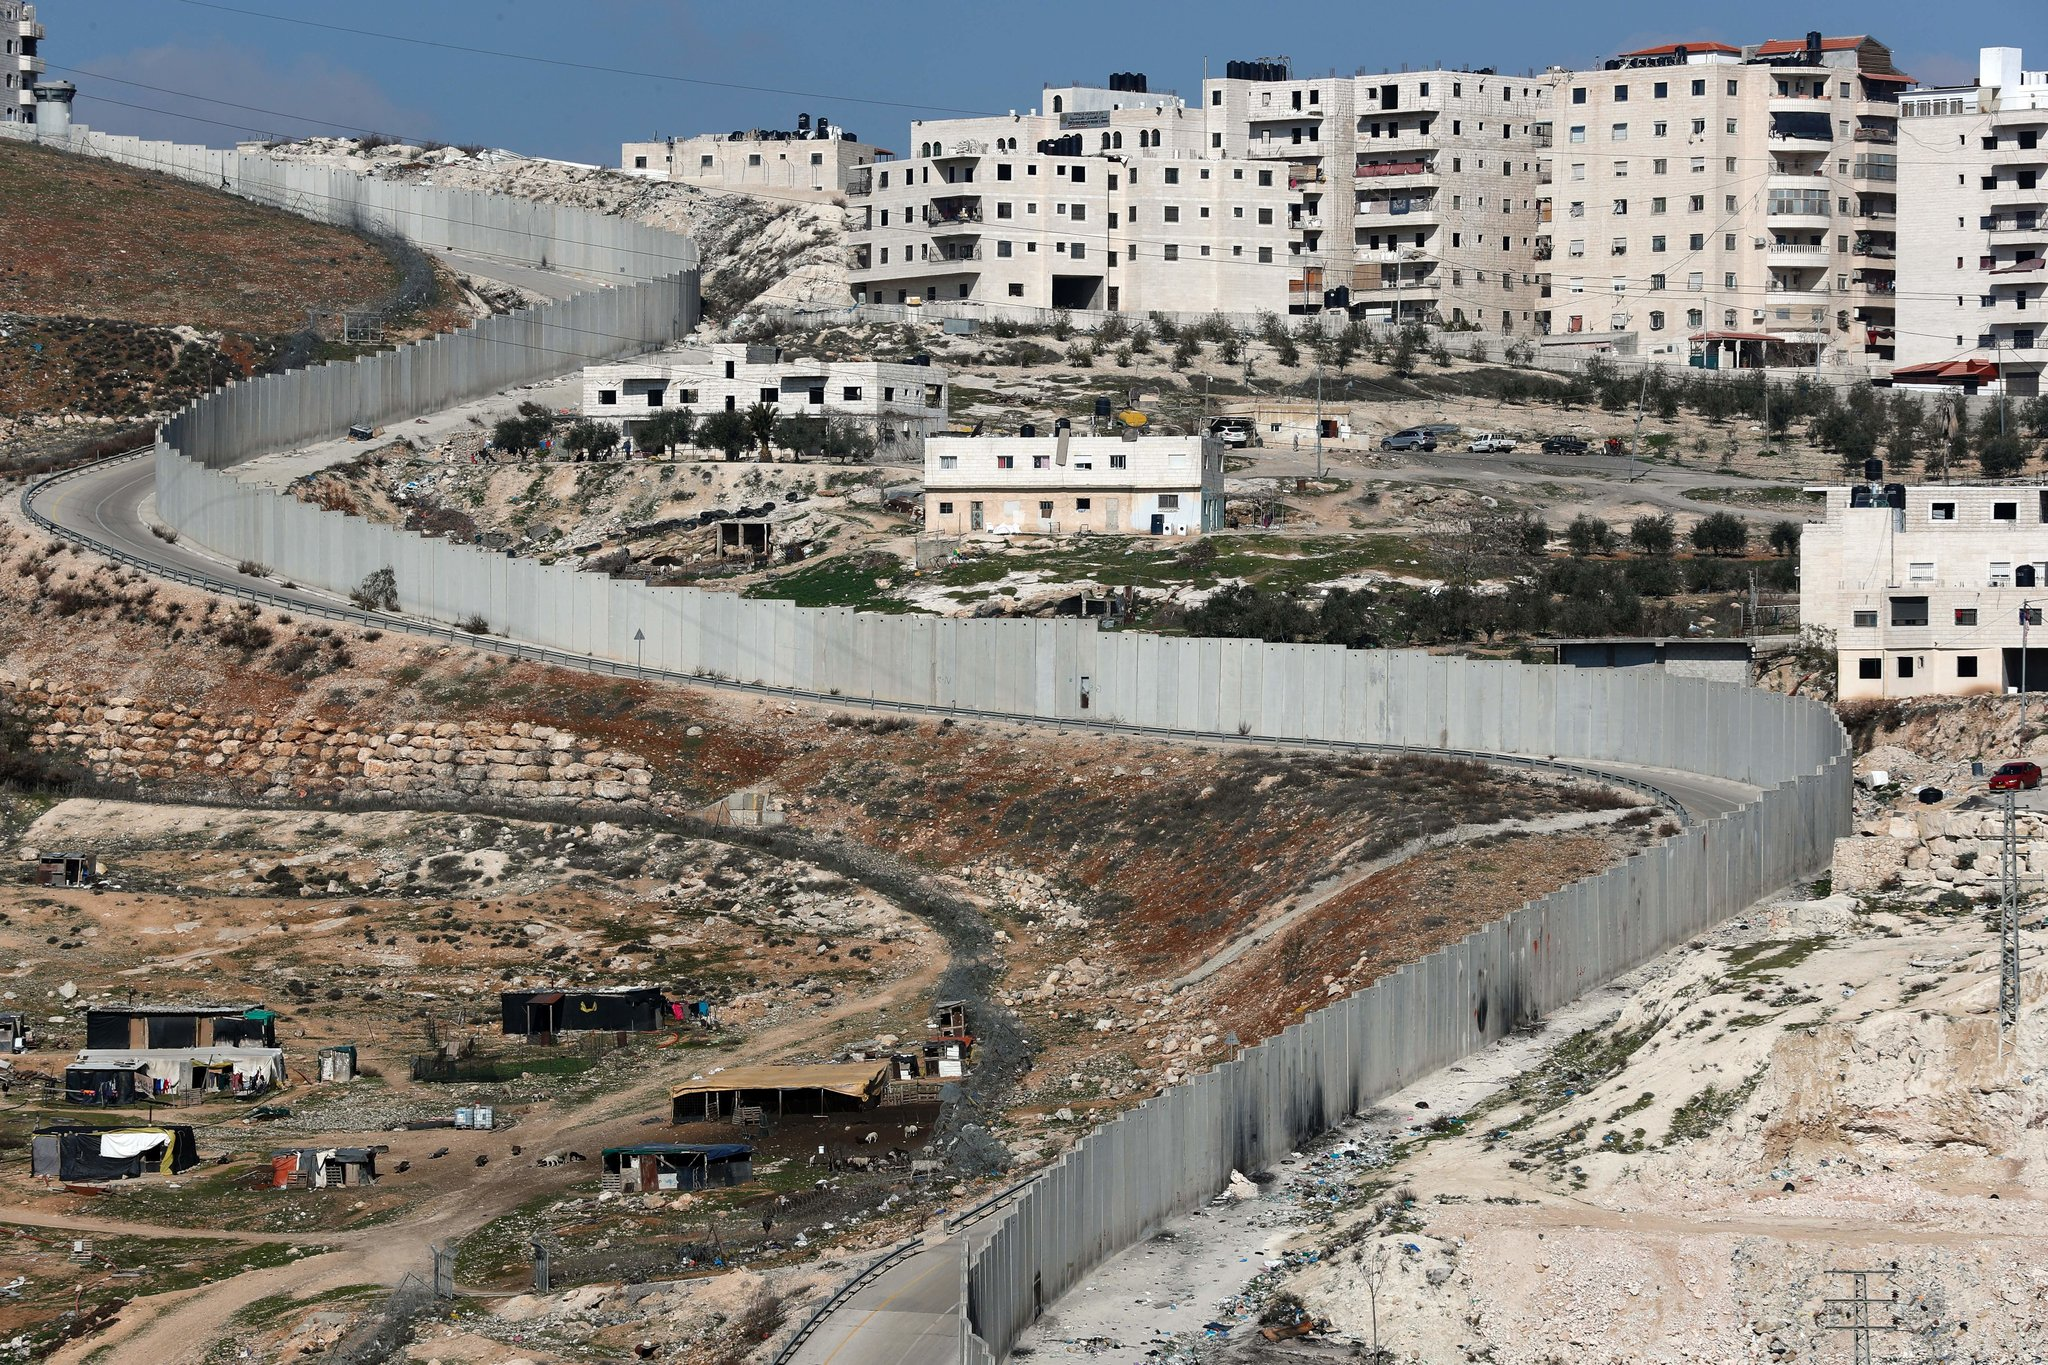
\includegraphics[width=1\linewidth]{separation-barrier-nyimes.jpg}
    \caption{The separation barrier dividing east Jerusalem, left, from the West Bank village of Anata. Thomas Coex/Agence France-Presse — Getty Images. From: \url{https://www.nytimes.com/2017/05/02/opinion/a-first-step-to-peace-calm-angers-then-talk.html}}
    \label{fig:separation-barrier}
\end{figure}

\begin{figure}
    \centering
    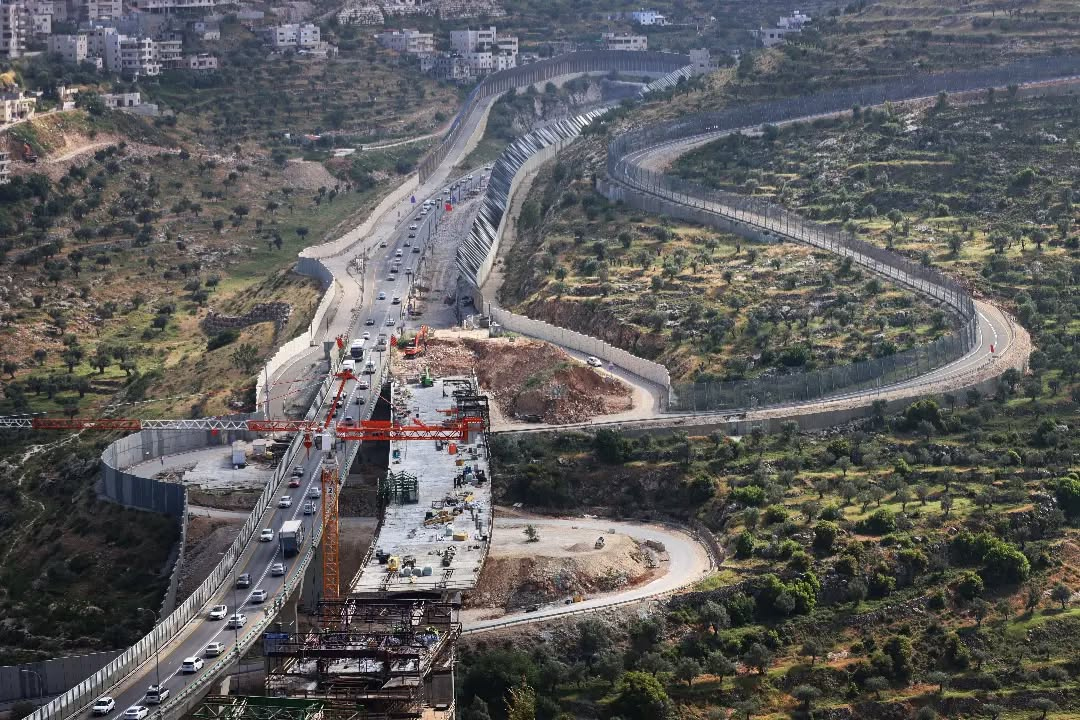
\includegraphics[width=1\linewidth]{gilo_bridge.jpg}
    \caption{The 'tunnel road', Photographed by Ahmad Al-Bazz, summer 2021. From: https://www.instagram.com/p/CcNVS1Vt6wO/}
    \label{fig:tunnel_road}
\end{figure}

\begin{figure}
    \centering
    \includegraphics[width=1\linewidth]{apartheid_road.png}
    \caption{The 'apartheid road', Photographed by Ahmad Al-Bazz, 31 March 2022. From: \url{https://www.nrc.no/shorthand/stories/in-the-west-bank-segregated-roads-displace-palestinians/index.html}}
    \label{fig:apartheid-road}
\end{figure}

% Ask permission fro Ahmad Al-Bazz?
\section{Intergroup Contact}
Pertinent to this dissertation, the original contact hypothesis and the majority of the research that followed do not deal with protracted, violent, and asymmetric conflicts such as the Israeli-Palestinian conflict. Maoz \cite{maozDoesContactWork2011} analyzed contact interventions between Israeli Jews and Palestinians between 1988 and 2008. They found that they could be classified to four different models, each with its own advantages and disadvantages: 1) Coexistence, 2) Joint Projects, 3) Confrontational, and 4) Narrative/Storytelling. The challenge of such contact interventions is to balance the level of directness with the substance of the conflict. When the encounter focuses on reconciliation, benign activities, and finding commonalities, it tends to neglect and diffuse existing grievances, asymmetric power relations, and injustices. This ignores the strong needs of the groups to tackle and express their difficulties, especially within disadvantaged groups \cite{maozMultipleConflictsCompeting2000,shnabelNeedsbasedModelReconciliation2008}. Moreover, when such contact succeeds, it tends to decrease the likelihood of participants from disadvantaged groups to promote social change that fixes existing injustices \cite{durrheimIntergroupContactStruggle2018, dixonOptimalContactStrategy2005, albzourTalkingSegregationWall2022, bekermanRethinkingIntergroupEncounters2007}. When the encounter takes the opposite approach and is focused on confrontation, it is naturally more likely to degrade into violence \cite{maozTheyUnderstandOnly2007}, eventually worsening the relations between the groups. Persistent confrontation may also alienate the Jewish participants (the advantaged group) from the discussion and reduce their motivation to join such activities. The difference here between the advantaged and disadvantaged group is also reflected in the "needs-based model" of Shnabel and Nadler \cite{shnabelNeedsbasedModelReconciliation2008,nadlerIntergroupReconciliationInstrumental2015, shnabelChapterFourNeedsbased2023}. According to this model, the disadvantaged ("victim") group in a conflict has a heightened need for empowerment and restoration of agency (which could manifest through direct confrontation of injustices), while the advantaged ("perpetrator") group has a need for acceptance and restoration of moral image (which could manifest as a will for coexistence). However, the authors note that the binary division is not absolute and in conflicts such as the Israeli-Palestinian conflict, members of the advantaged group may feel as victims and vice versa.

Maoz proposes the Narrative/Storytelling model as an attempt to achieve a balance of the needs by combining the advantages of both coexistence and confrontational models \cite{maozDoesContactWork2011}. In this model, participants share an intimate experience by telling their personal story about the conflict and its consequences. This approach was found to promote trust and empathy between participants, while not losing reference to the core of the conflict and existing social injustices \cite{bar-onConciliationStorytellingVictimhood2002,bar-onTellYourLife2006,bar-onStorytellingWayWork2004}. However, the same issue of balance occurs in the storytelling process. Participants struggle to find the 'good enough' story - one that contains commonly shared elements that promote empathy, but also contrasting perspectives that provoke thought without alienating listeners \cite{bar-onTellYourLife2006}. In this dissertation, we introduce an approach that uses theater and shares characteristics with the Narrative/Storytelling model. We develop the model further by including participatory telerobotic design as a collaborative and educational process, and as an enabler of remote digital contact between the groups. But first, we go into detail on aspects of intergroup contact theory and its branches that are relevant for this research.

\subsection{Group categorization and the dual identity strategy}
\label{sec:dual_identity}
As mentioned in the Introduction, Allport's original conditions for successful contact have been tested and verified through countless experiments over the years. However, researchers have developed the theory further in multiple directions. One direction pertains to the process in which group categories are modified or dissolved through contact. Three influential models on this aspect were developed: 1) the Gaertner and Dovido model of common ingroup identity \cite{gaertnerReducingIntergroupBias2000}, 2) the Brewer and Miller model of decategorization \cite{brewerContactHypothesisTheoretical1984}, and 3) the Hewstone and Brown model of category salience \cite{hewstoneContactNotEnough1986}. Gaertner and Dovido suggest that prompting participants to view themselves as members of a new common group gradually reduces the previous intergroup bias in a process called "recategorization". This could be a superordinate group, for example, women Israeli Jews and Palestinians who collaborate as part of the larger women group, or a new common group where participants collaborate on some tasks \cite{gaertnerCategorizationRecategorizationIntergroup2005} (as supported by Allport's conditions). Brewer and Miller emphasize the need to decategorize group members by acquaintance, confronting their personality with exiting known stereotypes. Decategorization is also facilitated by personalization - promoting more personalized and intimate relations between group members through mutual self-disclosure \cite{millerPersonalizationPromiseContact2002}.

Although these approaches were proven in multiple experiments, Brown and Hewstone argued that the reduction of prejudice and the improvement of attitudes between individuals in contrasting groups do not guarantee that the effect would be generalized to the outgroup \cite{brownIntegrativeTheoryIntergroup2005}. In other words, if an Israeli Jew and a Palestinian meet and end up with more positive opinions and less prejudice toward one another, will they feel the same toward the next stranger they meet from the same outgroup? They determined that the generalization depends on the "category salience" (also known as the "group salience") \cite{brownChangingAttitudesIntergroup1999,brownIntegrativeTheoryIntergroup2005}. When the group association of the individuals is prominent in the encounter, it is more likely that positive effects are generalized to the group level. This may at first sound counterintuitive, as it implies highlighting the differences between the individuals rather than focusing on commonalities, but Brown and Hewstone contend that this is essential for persisting the cognitive shift and can work when combined with the other conditions for positive contact.

As a response to the findings by Brown and Hewstone, Gaertner and Dovido suggested an extension to the common ingroup identity model - a "dual identity" strategy \cite{gaertnerCategorizationRecategorizationIntergroup2005, brownIntegrativeTheoryIntergroup2005}. The premise for this strategy is that it is possible to highlight a common group association and an outgroup association at the same time during contact. According to the authors, this occurs "when group identities and their associated cultural values are adaptive, or when they are associated with high status or highly visible cues to group membership" \cite[p. 80]{gaertnerCategorizationRecategorizationIntergroup2005}. The dual identity strategy is explored today not only because of its potential to promote the generalization of positive effects to the group level but also because of its role in promoting collective action and social change; we discuss this branch of the research in the next section.

\subsection{Collective Action and Social Change}
The previous section describes the shift in focus of intergroup contact research from reducing prejudice toward individual members of a group to generalizing and persisting that reduction in future encounters with members of the outgroup. However, in the context of asymmetric conflicts in which one advantaged group has structural superiority over the other, contact should also motivate participants to strive for a more equal society with fewer grounds for conflict between the groups. Recent research found that positive contact does not necessarily promote positive social change. In fact, it may be counterproductive by diminishing collective action \cite{saguyIronyHarmonyIntergroup2009,dixonLetThemEat2010,dixonPrejudiceAreNegative2012}. This is referred to in the literature as the "sedative effect" of intergroup contact \cite{cakalInvestigationSocialIdentity2011} - participants, in particular those of disadvantaged groups, gain a favorable attitude toward the outgroup and a more optimistic view of the social situation, which in turn decreases motivation for collective action, such as joining protests or advocating in public. In the context of the Israeli-Palestinian conflict, this notion is discussed in Palestine at least since the beginning of peace negotiations between the Palestinian authority and the state of Israel in the early 1990s \cite{miariAttitudesPalestiniansNormalization1999}. Many Palestinians believe that normalizing social relations with Israel before injustices are dealt with harms the Palestinian effort to achieve self-determination. Now, when intergroup contact research shifts focus to promoting collection action, it reifies this reasoning \cite{albzourSupportNormalizationRelations2019}.

Critical views on collective action gave rise to new models that seek the conditions in which intergroup contact promotes support for social change. The Intergroup Contact Collective Action Model (ICCAM)\cite{hasslerIntergroupContactSocial2021} reviews existing research and produces a model that outlines these factors. The model differentiates between advantaged and disadvantaged groups and, in fact, corresponds to the needs-based model of Shnabel and Nadler \cite{hasslerNeedSatisfactionIntergroup2022,shnabelChapterFourNeedsbased2023}. It was found that when group-specific needs are met (acceptance for the advantaged group and empowerment for the disadvantaged group), the motivation of group members for social change increases. Furthermore, the salience of group differences and their systemic illegitimacy was found to increase motivation for social change in both groups. The authors add that the dual identity model of Gaertner and Dovido is especially useful for maintaining support for social change while increasing empathy between the groups. This was also supported by the review by Cocco et al. \cite{coccoMobilizingSedativeEffects2024,banfieldWhitesPerceptionsDiscrimination2013} on intergroup contact and collective action. In summary, state-of-the-art research on intergroup contact highlights the positive effect of the dual identity and needs-based models for reconciliation between groups while maintaining motivation for social justice in asymmetrical conflicts.

\subsection{Indirect contact with digital technology}
\label{sec:indirect_contact}
Allport's original contact hypothesis in 1954 \cite{allportNaturePrejudice1954} referred to direct face-to-face meetings of group members and its potential to reduce prejudice. Since then, research has expanded forms of contact that are indirect \cite{whiteDirectContactTheoretical2021}, such as extended contact (having friends who have friends in the outgroup) \cite{wrightExtendedContactEffect1997,zhouExtendedContactHypothesis2019}, vicarious contact (observing contact between groups) \cite{gomezVicariousIntergroupContact2008,vezzaliImprovingIntergroupRelations2014}, and digital contact (contact mediated by digital technology) \cite{pereiradacostaDoesDigitalIntergroup2024}. The immediate advantages of indirect contact forms are their practical ease of setup and their potential to reach wider audiences than with direct contact. In addition, the research found qualitative advantages of indirect contact, such as having reduced anxiety due to the less intimate nature of the encounter, which could lead to a more positive outcome \cite{whiteDirectContactTheoretical2021}. Research on digital contact has evolved over the years from simple text-based communication to immersive and embodied experiences in virtual reality (VR). We propose a new medium for indirect digital contact, telerobotics. In this section, we review theoretical developments in digital contact, pointing out key remaining gaps and challenges that we attempt to address in our design.

Digital contact is an umbrella term for multiple types of contact that utilize digital technology. In a meta-analysis, Da Costa et al. \cite{pereiradacostaDoesDigitalIntergroup2024} identify three broad categories: 1) Contact based on computer-mediated communication (CMC), where group members interact "live", through a digital medium such as social media, text-based chat, video conferencing, or a game environment (see \cite{whiteTextbasedEcontactHarnessing2020,imperatoAllportMeetsInternet2021,amzalagImprovingIntergroupRelations2021,amichai-hamburgerContactHypothesisReconsidered2006, benatovGamingPeaceVirtual2021}), 2) Contact with an NPC, where ingroup members interact with a simulated or prerecorded outgroup member (see \cite{haslerVirtualPeacemakersMimicry2014,kabiljoVirtualRealityFostering2019}), and 3) Perspective taking, where ingroup members assume the identity of the outgroup member and experience reality through their perspective, typically in a virtual reality setting (see \cite{hassonEnemysGazeImmersive2019} an example). In this dissertation, we focus on the CMC type of digital contact, as the design we propose involves live communication mediated by telerobotics. 

Apart from reduced anxiety due to the indirectness of the encounter, digital contact of the CMC type has the unique quality of allowing participants to shape their identities in the digital conversation and control the level of exposure of their true self. Research suggests that both identifiability and anonymity could have benefits and drawbacks for intergroup contact, and there is no conclusive formula for an optimal balance \cite{haslerOnlineIntergroupContact2013, imperatoAllportMeetsInternet2021, whiteTextbasedEcontactHarnessing2020}. When supported by the context of the conversation, anonymity (or controlled identity) can increase the salience of the group over personal identities (see the social identity model of deindividuation effects or SIDE \cite{reicherSocialIdentityModel1995}). This could facilitate the discussion of group relations and stereotypes, empower members of disadvantaged groups to rise above existing power relations, and support the generalization of prejudice reduction to the group level \cite{kleinSocialIdentityPerformance2016,spearsWhenAreNet2002}. On the other hand, when the context does not support constructive discussion, anonymous conversations can result in more negative attitudes \cite{whiteImprovingIntergroupRelations2015}, as was seen in spontaneous online arguments between Israeli Jews and Palestinians \cite{ellisOnlineArgumentIsraeli2007}. Higher identifiability is also beneficial by increasing the overall engagement of participants in the conversation, therefore the potential to form lasting positive attitudes about the conversation partner and their group \cite{schumannWhenComputermediatedIntergroup2017}.

\subsection{Virtual Reality as an epitome of intergroup contact's shortcomings}
\label{sec:vr_empathy}
When considering the level of engagement in the conversation, a critical factor is \textit{social presence}. Originally coined by Short et al. \cite{shortSocialPsychologyTelecommunications1976}, the term refers to the degree to which parties that communicate over a digital medium sense that the social interaction is real. This perception was found to promote trust and intimacy in conversation, which are key factors that enable positive contact \cite{schumannWhenComputermediatedIntergroup2017}. Insofar as the digital medium lacks elements that are natural in face-to-face, such as nonverbal cues and gaze coordination \cite{kendonConductingInteractionPatterns1990}, social presence is reduced. Research shows that the richness of the media (such as the difference between a text chat and a video call) promotes social presence, as it supports the use of nonverbal cues \cite{newberryMediaRichnessSocial2001}. In terms of media richness, virtual reality (VR) provides a heightened experience that is also embodied \cite{slaterInfluenceBodyMovement1998} - Participants in a VR-based interaction can use their body to communicate in the virtual medium as they would face-to-face. Creators and journalists initially praised VR as the "ultimate empathy machine" \cite{milkHowVirtualReality2015}, allowing participants not only to see the virtual other in a full, embodied presence, but even to see themselves \textit{as} the other, from the other's perspective. However, a growing number of critics point out that as much as such experience can be moving and powerful, their overall effect on society is doubtful and possibly negative. Such criticisms are summarized in the ethnographic account of Lisa Messeri \textit{In the Land of the Unreal} (\cite{messeriLandUnrealVirtual2024}. Since VR (or XR, mixed reality) is considered an emerging state-of-the-art medium for digital contact \cite{chenFuturePrejudiceReduction2024}, it is worth reviewing its current research state as a background for this dissertation.

To my knowledge, despite the proven potentials of live CMC encounters, all VR-based intergroup contact initiatives except one \cite{tassinariInvestigatingInfluenceIntergroup2022} are of one of the other two types: contact with an NPC (virtual agent) or taking the perspective of the outgroup \cite{chenFuturePrejudiceReduction2024, tassinariUseVirtualReality2021}. This is likely due to the ease of setting up such experiences in a controlled and reproducible manner without losing their effect. Systematic reviews of research up to this point show mixed results \cite{chenFuturePrejudiceReduction2024, tassinariUseVirtualReality2021}. Although there are promising reports of an improvement in attitudes, negative effects of VR-based contact are also reported. This is in part due to the lack of research standards and a variance in the quality of the experience \cite{tassinariUseVirtualReality2021}, but critics \cite{messeriLandUnrealVirtual2024, nashVirtualRealityWitness2018, bollmerEmpathyMachines2017} point out an inherent fault in contact with the outgroup when it is either a simulation (with a virtual outgroup agent) or an assimilation (taking the role of the outgroup). In both cases, it can be seen as a form of dehumanization. According to this critique, even if an encounter promotes empathy, that sentiment is aimed toward a contrived figure of the other, a fantasy of contact. Such an experience redeems the participants from having to confront real members of the outgroup and therefore remains in a "virtual" comfort zone. 

How do we then reconcile with the increasing number of researchers who tout VR as a tool for a long-term improvement of intergroup relations? First, we should note existing issues with longitudinal research in the field of intergroup contact, challenging the presumption that positive contact promotes a persistent change in group members. As explicated by O'Donnell \cite{odonnellTechnologicalAnalyticalAdvancements2021} and Dixon and McKeown \cite{dixonNegativeContactCollective2021}, the majority of longitudinal contact research does not apply robust statistical methods, combining between-subjects and within-subjects comparisons, to adequately capture the cognitive change within participants. For example, all longitudinal VR research papers sampled from the aforementioned reviews \cite{herreraBuildingLongtermEmpathy2018,loonVirtualRealityPerspectivetaking2018,hassonEnemysGazeImmersive2019} use between-subject analyzes. More significantly, there is a gap in VR-based contact research that points to a more broad lack in the field, the focus on benevolence as the ultimate goal of contact. Louis et al. \cite{louisEmergingResearchIntergroup2019} make an important distinction between two different types of intergroup prosociality. Benevolence is associated with expressions of sympathy and empathy for the outgroup, such as charitable giving. These measures are commonly sought for in VR-based contact research (for example, \cite{loonVirtualRealityPerspectivetaking2018,derricoProsocialVirtualReality2020, branhamVirtualImmersiveContact2024}). However, while benevolence may promote social change indirectly by supporting a disadvantaged group, it does so without actively challenging existing systemic inequalities. Benevolence, as opposed to activism, addresses the symptom rather than the cause of the problem \cite{louisEmergingResearchIntergroup2019}. Moreover, a helping behavior that does not recognize systemic causes may reinforce power relations, decreasing the will for social change \cite{nadlerInterGroupHelping2002}. 

We find ourselves circling back to the contemporary debate on intergroup contact and collective action. VR, seen as a cutting-edge technological tool to create empathy and promote peace between groups in conflict (without involving living members of the disadvantaged group), acts as an epitome for the problem of linking intergroup contact to collective action and social change. Prejudice reduction and empathy can be positive drivers, and collective action and prejudice reduction are not mutually exclusive \cite{abramsPrejudiceReductionCollective2012}, but by focusing only` on empathy, benevolent behavior, and by neglecting the inclusion of the outgroup (typically the disadvantaged group \cite{messeriLandUnrealVirtual2024}) in the reconciliation process, the medium becomes prone to the negative effect of reinforcing power relations and the sedative effect. In terms of online or digital contact, research on collective action is still lacking. To our knowledge, there are only two studies that focused on CMC-based contact and collective action \cite{enicOnlineContactsSupported2024, schumannWhatCanBe2022} and no study that focused on digital contact with an NPC or virtual perspective-taking. An additional hypothesis is found in the DIEC program study \cite{whiteAchievingTwelvemonthsIntergroup2014} that examines the role of the dual identity strategy in text-based CMC in promoting a long-term reduction of prejudice. The study also notes the potential of the strategy to support collective action. An in-depth inquiry of these studies provides a gateway to the final and enclosing aspect of intergroup contact that we address in this dissertation, the content of contact.

\subsection{The Content and Length of Contact}
According to \cite{schumannWhatCanBe2022} the \textit{Connect Global} program, which holds video, audio and text sessions with students from different identity groups around the world, was able to predict a sustained reduction of prejudice and, significantly, tendencies for collective action on behalf of the outgroup. In contrast, the online text-based experiment of \cite{enicOnlineContactsSupported2024} also improved intergroup attitudes but did not increase collective action intentions. There are ostensible differences between the two interventions. In \cite{enicOnlineContactsSupported2024}, members of the advantaged and disadvantaged group who live in the same city collaborated in one event to solve environmental problems in their city. The task was not related to the difference between the groups (higher and lower status universities), but the authors used a dual identity model by changing the text chat nicknames of the participants to reflect the group ("ATU student \#1", "CU student \#2", and so forth). In contrast, the Connect Global program has weekly meetings over the course of eight weeks, and participants, identified by their nationality and background, discuss social issues directly such as "the global economy and inequality; stereotypes and cultural misunderstanding; global, local, and interpersonal conflict". Traditionally, this format is more associated with long-term peacebuilding programs than with contact interventions. Nevertheless, connecting back to the conclusions of Maoz \cite{maozDoesContactWork2011}, the change in trends in contact research in the past decade clearly shows that it is crucial to merge these two approaches, especially in protracted conflict and asymmetric conflicts.

A recent review by Cocco et al. \cite{coccoMobilizingSedativeEffects2024} analyzed 134 studies of intergroup contact in search for factors that affect collective action within advantaged and disadvantaged groups. A key finding is that the content of the contact is crucial. According to the findings, when the contact includes the discussion of group differences and the illegitimacy of inequalities, it promotes mobilization in both the advantaged and disadvantaged groups. Our review of the literature found very limited exploration of this aspect within digital contact. From instances involving real and organized communication between group members, the content of contact is usually a collaborative game (for example, \cite{stiffPlayingWellOthers2020, tassinariInvestigatingInfluenceIntergroup2022, benatovGamingPeaceVirtual2021}, including the single VR-based CMC intervention) or an educational task (for example, \cite{waltherComputermediatedCommunicationReduction2015,enicOnlineContactsSupported2024, whiteDualIdentityelectronicContact2012}. Although Coco et al. did not include the duration of the intervention as a moderator, they mention the importance of longitudinal research, not just to explore long-term effects, but also because longer interventions can reduce initial anxiety and create stronger relationships \cite{troppAdaptationDiversityIndividual2019, macinnisHowCanIntergroup2015,pettigrewAdvancingIntergroupContact2021}, factors that could eventually promote collective action \cite{coccoMobilizingSedativeEffects2024}. Although not explicitly stated, we can hypothesize that longer interventions make it easier to include more sensitive topics without causing too much anxiety, and that those sensitive topics eventually mobilize collective action. Because digital contact interventions allow controlled exposure of participants, they gain additional benefit from long-term interventions, providing more granular control to reduce anxiety \cite{amichai-hamburgerStructuredUnstructuredIntergroup2015}. This was also demonstrated in \cite{segalGoingHybridUsing2022}, where a six-month multistage online and on-site peacebuilding program was shown to increase participants' motivation for collective action.

\section{Participatory Design and Theater}
\subsection{The Roots of Participatory Design and Participatory Action Research}
Participatory Design (PD) \cite{disalvoCommunitiesParticipatoryDesign2012} and Participatory Action Research (PAR) \cite{falsbordaAccionConocimientoComo1991} are two research streams that have developed in parallel and share a common value of doing research collaboratively and equally with participants toward a social good. Both streams make use of Action Research (AR) \cite{lewinActionResearchMinority1946}, research that is explicitly conducted for the active improvement of the participants' life, rather than passive observation, and both have roots in Marxist thought. Significantly, both draw inspiration from Paulo Freire's "Pedagogy of the Oppressed" \cite{freirePedagogyOppressed2000} (see \cite{falsbordaAccionConocimientoComo1991} and \cite{ehnWorkorientedDesignComputer1988}). In a manifesto on education and power relations, Freire argues that teachers should see their students as collaborating subjects, rather than passive receptacles of knowledge. Teachers and students should engage in mutual learning, study societal structures from multiple perspectives, and challenge forms of oppression embedded in them.

Although technology has been used in PAR (especially among youth) \cite{gibbsUsingTechnologyScale2020}, its roots are in sociological research that empowers marginalized communities \cite{falsbordaAccionConocimientoComo1991,whyteParticipatoryActionResearch1991}. However, PD is more explicitly associated with the democratic design of technology. It originated in Scandinavia in the 1970s when computer science researchers collaborated with worker unions, allowing workers to participate in the design of the technological tools they would use \cite{kensingHeritageHavingSay2012}. Workers could propose an alternative technological vision to the one set by management and system engineers that was predisposed to automating the workers' role and alienating them from the work. The cornerstone projects were the iron and metal project in Norway \cite{nygaardTradeUnionsNew1975}, and the DEMOS\cite{ehnLocalUnionInfluence1983}, DUE \cite{kyngSystemsDevelopmentTrade1982} and UTOPIA \cite{ehnToolPerspectiveDesign1986} projects in Sweden and Denmark.

The progression of PD is described in \cite{smithRoutledgeInternationalHandbook2025} as having four waves, the first wave being the work with the Scandinavian workers' unions described above. The second wave expanded the concept of participation from workers to \textit{users}, inviting the participation of any future technology user in its design and implementation (for example, the MUST method \cite{bodkerInvestigatingSituatedUse2014}). The third wave expanded to working with communities \cite{disalvoParticipatoryDesignCommunities2012}, including marginalized communities, hobbyists, and activists. For example, in the Malmö Living Labs in Sweden, university students collaborated with a group of young immigrants to design creative technological methods to spread their music \cite{bjorgvinssonAgonisticParticipatoryDesign2012}. In the contemporary fourth phase, named in \cite{smithRoutledgeInternationalHandbook2025} \textit{designing otherwise}, PD adopts more expansive critical frameworks to develop practices that address global challenges, such as a posthumanist approach to ecology \cite{frauenbergerEntanglementHCINext2020,heitlingerAvoidingEcocidalSmart2018} and a pluriversal, decolonial approach to politics \cite{smithPluriversalityDecolonisingDesign2024}. In \cite{clarkeDecolonisingParticipatoryDesign2022}, researchers collaborated with Bedouin activists in Palestine to design kits that were sent to villages around Palestine that were facing house demolitions. The kits asked young people in the village to express their thoughts on the situation and the findings were publicly shared in online media and exhibitions.  

\subsection{Agonistic Participatory Design and Peacebuilding}
Despite the activist nature of PD and the potential of technology to bridge distances, as in \cite{clarkeDecolonisingParticipatoryDesign2022}, the majority of research in conflict areas focuses on the empowerment of disadvantaged groups without involving the advantaged groups. Although this supports peacebuilding and equality by empowering the disadvantaged group, it is only part of the reconciliation process. In a recent statement by Pelle Ehn, one of the founders of the PD movement in Scandinavia \cite[p.293]{bodkerAfterthoughtsEmergentFuture2025}, he suggests that "Participatory Design activists should join forces with the peace movement", citing numerous ideas for how PD can help promote peace, one of which is "reinforcing local cross-border peace initiatives between people from Israel and Palestine". Ehn emphasizes that this should not result in one-time interventions or summit meetings, but a long-term commitment alongside peace organizations. There has also been a call from the field of intergroup contact to incorporate more participatory and qualitative methods. According to Dixon and McKeown, "there is an urgent need for in-depth qualitative studies to examine intergroup contact", including "discursive, participatory, and narrative methods" that "explore how participants themselves make sense of contact experiences" \cite{dixonNegativeContactCollective2021}. The authors cite an example from Suffia et al. \cite{sufflaPhotovoiceCommunityEngaged2012}, where youth participants in South Africa engaged in dialogue by taking photos and exhibiting them.

There are more explicit examples in the literature of participatory design interventions in areas of conflict or dispute. In Colombia \cite{patarroyoTestimonialDigitalTextiles2019} and Croatia \cite{jolicBottomupVsTopdown2023}, researchers and local communities used PD to define and process post-conflict memories and reconciliation. In Germany, young forced migrants (YFM) collaborated with German youth to design a geospatial application that supports the integration of YFM in the urban environment \cite{duarteParticipatoryDesignParticipatory2018}. As an example of working directly with a contested land, the project "Hands-on Famagusta" \cite{stratisReclaimingPoliticalUrbanism2017}, facilitated explorations of urban design of the city of Famagusta in Cyprus with Greek and Turkish Cypriots. The approach of the authors was "agonistic", inspired by the concept of Chantal Mouffe \cite{mouffeAgonisticsThinkingWorld2013} for a political space that encourages vibrant dissensus rather than consensus that suppresses the opinion of the dissent. Agonistic design \cite{bjorgvinssonAgonisticParticipatoryDesign2012, disalvoAdversarialDesign2015} sees design as creating "things" rather than objects \cite{binderDesignThings2011}, referring to the Old Norse etymology of the word "thing", an assembly where matters of concern are discussed. Thus, agonistic design things are creative opportunities for society to express social concerns, acknowledging a dominant hegemony, but echoing the voices of rival ideologies that challenge it. Although researchers note that existing power relationships (between different stakeholders) and protocols in agonistic design projects may inadvertently suppress marginalized voices \cite{buschBetrayalPostpoliticalParticipation2023, markussenDisruptiveAestheticsDesign2013}, the community is constantly refining the practice to adhere to the freedom and equality principles of agonism \cite{geppertDesignEquivalenceAgonism2022}.

The above PD interventions have not used the framework of intergroup contact, and there is limited exploration of the integration of these two fields. In \cite{rifatCohabitantDesignImplementation2024}, participants from different religions participated in the creation of a VR perspective-taking experience aimed at reducing prejudice toward a religious outgroup. However, although the authors refer to intergroup contact as a guiding theory for the creation of the app, they did not analyze the effect of contact between participants themselves during the design process. Conversely, in \cite{cheungEliminatingAgeismHigher2023}, PD was used to facilitate intergenerational contact between students and older adults, and the authors analyzed the effect of contact during the workshop, but the designed products, such as a travel assistant app and a Tai Chi motion capture, did not directly address issues between groups. A promising example for an integration of the discussed theories is found in a recent study on the multiethnic "Design Workshop" model that was employed by the government and municipalities in Thailand. In the workshops, participants of different ethnic groups co-designed spaces that reflected their municipality's multicultural nature while expressing the differences between their identities. The authors cite contact theory as well as the "social innovation theory" of Manzini \cite{manziniDesignWhenEverybody2015}, which stresses the capacity of PD to drive social innovation through multiple small-scale, interconnected, and open-ended design projects. The study in Thailand reports positive and sustained results, not only through contact between the participants but also through the impact of the designs on the local community. However, as the authors note, the study is based on two localized interventions that did not have a plan for continuous participation and requires further research. As in the intergroup contact research discussed earlier, PD researchers also found that long-term processes and commitments are needed to increase community engagement and social change \cite{saad-sulonenUnfoldingParticipationTime2018a}. In summary, while PD researchers have worked in contexts of intergroup conflict, the field has not reached the desired symbiosis with peacebuilding initiatives, as envisioned by Pelle Ehn. In particular, there is a missed opportunity for integration with projects that share the technological perspective of PD, such as the digital contact initiatives discussed in the previous section.

\subsection{Participatory Art and Theater of the Oppressed}
Participatory design shares its core values with participatory art \cite{holtTransformationAestheticArt2015}. Both are motivated by a vision of democratic citizen participation, inspired by Freire \cite{matarassoRestlessArt2019}, in which the community takes control over creating its future. As Holt shows \cite{holtTransformationAestheticArt2015}, some projects blur the lines between the two fields. The artist Jeanne van Heeswijk conducted community urban planning workshops as part of her artistic practice\cite{vanheeswijkInclusiveUrbanStrategies2011}. The aforementioned "hands on Famagusta" is also an example, as it participated in an art and architecture exhibition at the Venice Biennale \cite{stratisReclaimingPoliticalUrbanism2017}. PD researchers have also studied participatory arts to gain insight into the pitfalls of participation (for example, how participation might be co-opted by institutional and neoliberal agendas \cite{balaGesturesParticipatoryArt2018}), and the integration of HCI into participatory art \cite{holmerConstructingConstrainingParticipation2015}. Tselika \cite{tselikaConflictTransformationArt2019} has reviewed instances of participatory art that promote transformations in areas of conflict. In particular, the predominance of community theater is noted, with the use of theatrical techniques to create "contact zones" \cite{prattImperialEyesTravel2008}, essentially spaces for intergroup contact. Examples include a collaboration between the Greek Cypriot Satiriko Theater and the Turkish Cypriot Lefkoşa Belediye Tiyatros \cite[p.17]{tselikaConflictTransformationArt2019}, youth community theater in post-war Bosnia and Herzegovina \cite{zelizerRoleArtisticProcesses2003}, and community art initiatives in Northern Ireland (for specific examples of theater, see \cite{pierseCreativelyConnectingCivil2020}).

In every case of the participatory political theater research reviewed, the work of Augusto Boal and TO \cite{boalTheatreOppressed2008} is mentioned as a cornerstone \cite{pierseCreativelyConnectingCivil2020,epskampTheatreDevelopmentIntroduction2006, tselikaConflictTransformationArt2019, matarassoRestlessArt2019}. Boal, a fellow Brazilian to Paulo Freire, took the "pedagogy of the oppressed" and applied it to theater. In both cases, the foundation of the process is the breaking of the unidirectional, asymmetric relationship between educator and student, or for Boal, actor and spectator; the passive observers turn into equal, critical subjects.  In theater, this means that the spectators (the audience) become "spect-actors" and join the performance on stage \cite{boalTheatreOppressed2008}. Both methods also share the overarching political goal of unveiling oppressive societal structures through the participation of marginalized or silenced actors. For Freire, this is done with a dialogue in class. For Boal, this is done with improvisational theater. Alongside Freire, Boal's methods are influenced by Bertol Brecht and the Agit-Prop movement \cite[p.91]{friedmanPerformanceActivismPrecursors2021}. Agit-Prop (short for Agitation
and Propaganda) was a workers' theater movement in Soviet Russia that started with the revolution of 1917. The transformation of political power also sparked a transformation in the arts and theater \cite[p.97]{fischer-lichteTheatreSacrificeRitual2007}. Countless theater groups were formed by poor and working-class people who wanted to spread the revolutionary political message through original theatrical performances \cite[p. 17]{friedmanPerformanceActivismPrecursors2021}.

The influence of Agit-Prop spread beyond the borders of Russia and was a key element in the development of the "Epic Theater" method by Bertol Brecht. Brecht was a German Marxist, theater director, playwright, and theorist of the same period. He was inspired by the ability of Agit-Prop creators (working-class people without previous theater experience) to present complex ideas about existing social reality with original and daring artistic techniques \cite{brechtBrechtTheatreTrans1964}. In particular, he was impressed by their persistent focus on arousing political reflections within the audience, as opposed to emotional identification and empathy with the characters \cite{brechtBrechtTheatreTrans1964,friedmanPerformanceActivismPrecursors2021}. Significantly, Brecht's view of empathy as an element that stands in the way of social change resonates with the criticism of VR as an empathy machine and the focus on empathy in intergroup contact, as outlined in \hyperref[sec:vr_empathy]{Section 2.1.4}. Brecht's "Epic Theater" uses various theatrical methods that he calls "Verfremdungseffekt" (the "making strange effect"), replacing empathy with critical reflection, by creating a distance between the audience and the experience of the characters \cite{brechtBrechtTheatreTrans1964}. Verfremdungseffekt was a great inspiration for August Boal, but in contrast to Agit-Prop, Brecht still maintained the separation between actors on stage and spectators at the balcony. Boal wished to follow the political didactic methods of Brecht, but instead of encouraging spectators to think critically, he would invite them to act out their thoughts on stage; facilitating their social transformation \cite{boalTheatreOppressed2008}. Boal was a lead director of the Arena theater in São Paulo when in 1964 the political right took power via a military coup. The government hunted down left-wing theater groups, and Boal, forced to flee from place to place, formed underground theater movements in marginalized communities without professional actors. In 1971, Boal was captured by the regime and was sent to 15 years of exile. During a part of his exile in Peru, he developed the TO methods to aid in a governmental literacy campaign for poor and indigenous communities, including his most widely known method, "Forum Theater".

\subsection{Forum Theater in Peacebuilding and Design}
According to Boal, Forum Theater is the third and final degree in the transformation of a participant from spectator to spect-actor \cite{boalTheatreOppressed2008}. The premise of all stages is that the audience views a scripted scene played out by actors, typically depicting a certain social issue where the protagonist is in some way oppressed. The participants are then encouraged to propose a solution to the situation. In the first degree of intervention: \textit{Simultaneous dramaturgy}, participants intervene in a scene by proposing a new script for the actors to perform. In the second degree: \textit{Image theater}, the scene is frozen, and participants sculpt the ideal scene by moving the bodies of the actors, as well as a 'transitional scene', depicting how the scene transitioned from oppression to liberation. Finally, in Forum Theater, Boal would first ask the audience if they agree with the way the protagonist handled the situation in the scene. If not (the likely scenario), he invites them to play the scene differently, replacing the protagonist \cite{friedmanPerformanceActivismPrecursors2021, cohen-cruzBoalCompanionDialogues2006}. In this way, spectators become agents of their own freedom from oppression. 

The facilitator role in Forum Theater is defined as the role of the Joker \cite{boalTheatreOppressed2008}. Originally, Boal invented the "Joker system" during his time at the Arena theater to accommodate the goal of delivering a critical message at the expense of relinquishing theatrical consistency of style and cast. In the Joker system, actors can switch between different characters and styles to emphasize their role as interpreters of the play, not as fictional characters. In particular, the Joker actor bridges between the audience and the play by providing explanations and analyzes, interviewing the characters or the audience, interrupting the play, and taking over a certain character. Later, the Joker became a central part of Forum Theater, soliciting the audience to join the stage and play their own interpretation of the play. Boal perfected his facilitation methods during his 10 years of exiles in Europe from 1976 to 1986. In there, Forum Theater became a public performance in itself, rather than just a private workshop. In the book that followed, "Games for Actors and Non-Actors" \cite{boalGamesActorsNonActors2021}, Boal outlines a collection of games and techniques for future Jokers for Forum Theater. Boal adapted his methods to an audience that was not oppressed by a life-threatening authoritative regime, but by subtle internal and external forces of society \cite{cohen-cruzBoalCompanionDialogues2006}. This later developed into a therapeutical method described in the book "Rainbow of Desire" \cite{boalRainbowDesireBoal2013}. Boal finally returned to Brazil in 1986 and continued the use of Forum Theater methods in service of the new democracy, using "legislative theater" to generate ideas for new laws \cite{cohen-cruzBoalCompanionDialogues2006}.

Today, Boal's methods are seen as a subset of the broader term 'Applied Theater' \cite{gjaerumAppliedTheatreResearch2013}, encompassing all participatory theatrical activities that occur outside the traditional theater for social dialogue and education. There is a limited exploration in the literature for combining Boal's methods with intergroup contact theory. The methods have mainly been used as a pedagogical tool in the classroom, addressing topics such as racism \cite{abramsPrejudiceReductionCollective2012}, LGBTQ rights \cite{abramsPrejudiceReductionCollective2012,garciaOppressionPedagogyIntergroup2019} and stigmas of mental health \cite{nordstromVoicesProjectUsing2021}. A 2012 project in Palestine: Freedom bus \cite{riversNarrativePowerPlayback2015}, resonates with the criticism of intergroup contact interventions focusing on empathy and reconciliation while ignoring systematic inequalities, also citing concerns of normalization. In contrast, the project uses Playback Theater \cite{sajnaniOpeningPlaybackTheatre2011}, a form of applied theater that is partially inspired by TO, but focuses on the therapeutic and dialectic sharing of stories, rather than finding active solutions to combat oppression. In Freedom Bus, the theater is used to raise awareness and support the Palestinian struggle for justice. Although "Israeli activists have been welcome guests" at the events \cite[p. 159]{riversNarrativePowerPlayback2015}, the interventions focus on the disadvantaged group. 

In the broader context of peacebuilding, applied theater and TO have been proposed as a playful and expressive method of dialogue and storytelling in post-conflict settings \cite{aguiarAppliedTheatrePeacebuilding2020}. For example, in post-war Liberia Forum Theater increased trust, the sense of community between groups, and the willingness to participate in collective action \cite{feuchteForumTheaterCan2020}. Furthermore, two similar revisions of Forum Theater were developed independently by researchers to accommodate the specific needs of intergroup conflict. In this context, instead of working with a homogeneous group that challenges a nonpresent oppressor, two groups in conflict participate, and every group may see the other as the oppressor.  Miramonti et al. \cite{miramontiForumTheatreReconciliation2025} developed the "Forum Theater for Reconciliation" (FTR) for a conflict in Bolivia between indigenous people and migrant peasants over the infliction of wildfires in the region. The format places emphasis on building trust and sharing narratives between opposing groups during the production of the play. Although a single scene usually contains one obvious oppressed protagonist and oppressor, the process allows the groups to discuss the complex and multifaceted nature of oppression in intergroup conflict. Facilitators also encourage participants to swap roles between groups and embody the position of the other side in the play. Finally, when the play is performed in public to a mixed audience of both groups, spectators are invited to replace both the oppressed protagonist and the antagonist of the oppressor in the play. This method solicits feedback from audience members of both groups on how they would act differently.

In Israel and Palestine, the Tel Aviv/Tul-Karem Activist Theater group (TA/TK) was founded in 2007 as a branch of the Combatants for Peace organization (CFP) \cite{alonCHAPTERFOURTEENNonViolent2011}, a movement for non-violent peace activism of ex-militants in Israel and Palestine. The group developed 'Polarized Forum Theater' as a Forum Theater that is "designed for mixed groups who have extreme conflict" \cite[p. 167]{alonCHAPTERFOURTEENNonViolent2011}. Here, too, the revised model allows spect-actors to replace both the oppressor and the oppressed, and encourages participants to switch their identity. They mention having discussed this format with Boal and receiving approval for the method \cite[p. 167]{alonCHAPTERFOURTEENNonViolent2011}. As in \cite{miramontiForumTheatreReconciliation2025}, allowing the replacement of the oppressor in the scene could reveal the complexities of how the oppressors themselves feel oppressed. For example, an Israeli soldier feeling forced to do their role of oppressing a Palestinian citizen. Crucially, the TA/TK theater also dealt with real physical danger. Since "there are few places now (in 2010) where Israelis and Palestinians are allowed to gather together", the group used "trespassing" as a strategy and held public performances near military checkpoints outside of Palestinian villages \cite[p. 170]{alonCHAPTERFOURTEENNonViolent2011}. One time, this resulted in the actual attempt of arrest of a Palestinian who was playing an Israeli soldier for "contempt of the Israeli Defense Force (IDF) uniform" \cite[p. 171]{alonCHAPTERFOURTEENNonViolent2011}. Alon concluded that "there is no way to do 'conventional' Forum Theatre when the actors and spectators are in real danger, when there is no safe space for mutual learning, for true interaction between the play and the spect-actors" \cite[p. 172]{alonCHAPTERFOURTEENNonViolent2011}.

The tools of TO have been explored for the use of participatory design \cite{macchiaExploringTheaterOppressed2016}. In the University of Dundee, a playwright in residence was recruited to experiment with TO in design. In \cite{morganRequirementsGatheringDiverse2008}, a method similar to Simultaneous Dramaturgy was used to gather requirements for a telecare application for the elderly. The audience viewed a scene of a user interacting with the technology, debated the issues that were posed, and proposed changes. In \cite{riceForumTheatreRequirements2007,newellUseTheatreRequirements2006}, although the audience did not replace the characters, the participants interviewed the actors about the technology while they remained in character. In the work of Vines \cite{vinesExperienceDesignTheatre2014, vinesPlayingProvocations2018} a similar approach was used in the design of a net care app, in what they refer as Experience Design Theater. The two main differences were that the author used a more iterative approach, integrating the discussions with the participants into the theater scenes, and that the plays were focused on the experience and relations of the characters in the whole process of using the technology, not just its technical interface. Finally, in a project inspired by the TO approach of promoting participation for social good, Flanagan and Nissenbaum created a toolkit to incorporate activist values into game design and used it to design a dancing game that teaches programming to girls \cite{flanaganGameDesignMethodology2007}. There is no known research using TO for the participatory design of intergroup interventions or other peacebuilding technologies. 

\section{Telerobotics and Puppetry}
\subsection{Telerobotics and telepresence}
The first article in this thesis contains a detailed review of telerobotic research that considers every aspect of telerobotic design, such as appearance and functionality, toward its integration as a medium for intergroup contact. In here, I present a more broad and up-to-date overview of the field, focusing on its key relations to the thesis and research done since the publication of the articles. First, it is essential to examine the history of the terminology used in the field to understand the framing of this thesis. In 1980, Marvin Minsky popularized the term "telepresence", coined by his friend and futurist Patrick Gunkel \cite{minskyTelepresence1980}. Minsky's vision was about the future of what was known as "teleoperator technology". According to Minsky, the advanced remote operation of telerobotic devices, such as space shuttle arms or surgical tools, marks the first step toward a technology that could enable a human to feel entirely present in a remote location, perform complex tasks in hazardous environments, and work in different places without transportation. This could be achieved with the development of fine-grained control and feedback mechanisms that mirror every motion of the human to the robot, and every sense of the robot back to the human, thus achieving telepresence.

In 1995, Sheridan published a "progress report" on teleoperation, telerobotics, and telepresence \cite{sheridanTeleoperationTeleroboticsTelepresence1995}. He defined a telerobot as "any semiautomatic machine which has artificial sensors, actuators, and a computer, and is controlled in supervisory fashion" \cite[p. 205]{sheridanTeleoperationTeleroboticsTelepresence1995}. Sheridan noted that although research on telerobotic technology and telepresence was still relevant (especially in Japan), there is an increase in research on "virtual presence", the phenomenon of being present in a virtual world, driven by advancements in virtual reality and visualization technologies. In fact, some researchers have started to use the term "telepresence" also for virtual environments \cite{steuerDefiningVirtualReality1992}, and the overarching field of "presence" was being further developed in the context of virtual reality \cite{slaterInfluenceBodyMovement1998}. The resurgence of telepresence robots came with the COVID-19 pandemic that broke out in early 2020, which coincided with an increase in the commodification of telepresence robots \cite{shenRobotsCOVID19Pandemic2021}. Telepresence robots were used in a variety of social and daily tasks when people were quarantined and unable to leave their premises. This included remote work, education, health care, elderly care, and deliveries \cite{shenRobotsCOVID19Pandemic2021}. 

% TODO: An figure with a collection of images of telerobots?

However, this thesis refers to "telerobots" rather than "telepresence robots". The main reason for this shift, as I will show in this thesis, is that the technical solution presented for a remote puppet theater does not entail the sense of remote presence of the puppeteer. In fact, it is possible to operate a remote theater without perceiving the remote environment simply by setting up the remote location to mirror the puppet show performed locally. Furthermore, current research shows that the term "telepresence" has been declining, while its predecessor, "teleoperation", is gaining traction \cite{rosa-garciaBridgingRemoteOperations2025}. The exact cause of the shift is not clear, but a possible factor is the development of robot autonomy and AI, reducing the need for the teleoperator to be fully present in the remote environment \cite{darvishTeleoperationHumanoidRobots2023}. The use of telerobotics to mediate intergroup contact is to my knowledge so far unexplored.

\subsection{Puppets and Metaxis}
% About puppets and therapy
Puppets have been used as a tool by psychotherapists for decades as part of 'play therapy' \cite{aronoffPuppetryTherapeuticMedium1996}. Psychoanalyst D. W. Winnicot wrote of 'transitional objects' \cite{winnicottPlayingReality1991}, objects that exist in a safe, in-between space, that as part of play allow adults and children to express their feelings and thoughts without social inhibitions. Puppets are believed to exist in that space \cite{triminghamObjectsTransitionPuppet2010, wisniewskaHybridityPuppetry2020}. These properties contributed to the emergence of puppetry as a pedagogical tool \cite{krogerPuppetPedagogicalTool2019}, as well as a radical political tool, as with the 'Bread and Puppet Theater' in the US \cite{schumannRadicalityPuppetTheatre1991} and 'Puppets Against Apartheid' in South Africa \cite{krugerPuppetsPoliticsFinding2016}. The use of puppets in intergroup contact in the literature is limited to an imagined type of contact, such as children with refugees \cite{charalampidouInventingNewRoad2022}, immigrants \cite{jonesNoStringsAttached2020}, and homosexuals \cite{mausKindergartenChildrensAttitudes2025}. In the context of TO, Smith coined the term "Applied Puppetry" in 2014, creating an academic framework for applied theater research that uses puppetry as its medium \cite{purcell-gatesAppliedPuppetryCommunities2020}. Consequently, Laakkonen, in his work with palliative care, has expanded Boal's spect-actor term to spect-animator when using everyday objects and puppets as a form of expressive therapy with hospice patients. 

The most extensive exploration of puppetry and TO was done by Grant \cite{grantObjectsObjectivesApplied2020}. Grant had been working with applied theater and TO when he was introduced to the therapeutical and facilitating qualities of puppetry. The power lies in the phenomenon of "double vision" \cite{mortonHyperobjectsPhilosophyEcology2013} that occurs in puppet plays. Research shows that when puppeteers are visible, the audience can perceive and react both to the identity and presence of the actors, as well as to the identity and presence of the puppets. Moreover, when the puppeteers display an empathic connection to the puppets, their effect is transitive, and the audience can discern their emotion within the puppet and in relation to the happenings of the play. Grant acknowledges the similarity of this phenomenon to the desired "making strange" effect of Brecht. Puppets can enable the separation between actor and character that opens up the space for a critical discussion. However, through Boal, Grant shows how this quality expands beyond the didactic benefits of a political message. The "double vision" phenomenon, from the perspective of the puppeteers, has therapeutic value because it enables the actors to create a safe distance between themselves and the sensitive content that they are to reenact. This phenomenon is defined by Boal as "Metaxis" in the book "The Rainbow of Desire",  which focuses on the therapeutic aspects of TO \cite{boalRainbowDesireBoal2013}. Metaxis is "the state of belonging completely and simultaneously to two different, autonomous worlds: the image of reality and the reality of the image." \cite[p. 43]{boalRainbowDesireBoal2013}. According to Boal, the oppressed actor creates a safe rehearsal space (the image space, the play) for emancipation. When liberation occurs in the reality of the image, it can be extrapolated back to the real world (the reality of oppression).

Grant had witnessed this in effect in a workshop with the Tiger Bay Men's group in Belfast, 2014 \cite[p. 5]{grantObjectsObjectivesApplied2020}. The group consisted of men who were affected by the intergroup conflict in Ireland and specifically who experienced trauma related to suicide. It was led by Aja Marneweck, a puppet artist and facilitator who uses paper crumpling as a participatory puppet making method. Grant noted that "the puppet appeared to serve as a distancing device: this isn’t me telling the story; it’s the puppet telling it." \cite[p. 5]{grantObjectsObjectivesApplied2020}. This allowed participants to discuss themes that they were not able to discuss using verbal discussion alone. In addition, the empathic connection between the puppeteer and the puppet was clear; the group could easily understand the emotional relationship of the storyteller with the story. Significantly, puppets also empowered marginalized communities in an intergroup setting. In another workshop facilitated by Marneweck in Barrydale, South Africa, members of a colored community (including children and non-actors) perform in front of a white audience from neighboring towns \cite[p. 6]{grantObjectsObjectivesApplied2020}. The locals used a variety of puppets on various scales to tell their story and touch on sensitive themes such as slave trade. With and inside their puppets, the actors were being invisible and visible at the same time. The use of puppets here in an intergroup setting with the "double vision" effect resonates with the "dual identity model" of intergroup contact reviewed in \hyperref[sec:dual_identity]{section 2.2.1}. 

Finally, reflecting on a series of workshops, Grant acknowledges the power of puppets to channel emotional energy on a metaphysical level. Meaning, the materiality and functionality of the puppet have an agency of its own, which is driven by the emotional connection of the puppeteer (or multiple puppeteers of a single puppet) and then shared by anyone who witnesses the act. Marneweck sees this effect as part of a collective ritual of "radical empathy" \cite{marneweck2016a}, a deep intersubjective and performative connection of recognizing the pain of the other through the use of puppetry. The term is used by the anthropologist Joan Koss-Chioino \cite{koss-chioinoSpiritualTransformationRelation2006} in relation to spiritual healers who become a vessel for the pain of a stranger in a collective healing ritual - the community confronts the pain of the other through the mediating force of the healer. As suggested by Astles \cite{astlesWalkWalkMy2020}, puppets have this ability to act as a vessel and mediate radical empathy, which would be beneficial in the field of healthcare for both training and therapy. Significantly, radical empathy is described as a driver of collective action in favor of the other \cite{astlesWalkWalkMy2020}, making it the type of empathy that is highly sought after in the field of intergroup contact. 

\subsection{Robots and Theater}
Robots have a long history with theater, beginning from the 17th century, when the mechanical automata "Karakuri ningyō" robots were used for entertainment purposes in Japan \cite{knightEightLessonsLearned2011}, and leading to advanced puppet robots in Japan \cite{sakashitaYouPuppetEvaluation2017, kawaharaTransformedHumanPresence2016} and Taiwan \cite{huGlovePuppetRobot2008}. In the West, research is led by interdisciplinary researchers such as Elizabeth Jochum, who studies ways in which the inclusion of robots in the theater could promote HRI research \cite{jochumRehearsalRobotRevolution2014}. This includes the use of robots as puppets for an autonomous theater and the study of robot control mechanisms \cite{jochumRoboticPuppetsEngineering2014}, the use of theatrical robots to study the social dynamics of HRI \cite{katevasRobotComedyLab2015}, and the use of robotic theater for technology and art education \cite{bravosanchezInteractiveDramaRobots2017,dongChildRobotMusicalTheater2024}. Crucially, Jochum has pioneered the integration of TO and applied theater and robotics research in her study of care robots \cite{jochumUsingTheatreStudy2016}. Although the study did not use specific methods of TO and participatory theater, it was inspired by the notion of involving future care robot users in its design by providing feedback on a theatrical play. The audience watched a play about a woman with short-term memory loss and her assistive care robot (see Figure \ref{fig:cornell}). The engagement of the audience in the play was analyzed, and the participants completed a post-performance survey on various aspects of HRI and social robotics.

\begin{figure}
    \centering
    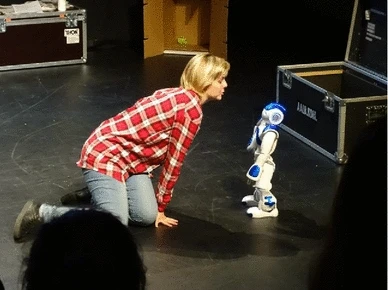
\includegraphics[width=0.7\linewidth]{jochum.png}
    \caption{The play Cornell as shown in \cite{jochumUsingTheatreStudy2016}, depicting the interaction between a human and their care robot. Audience feedback was used to study human-robot interaction.}
    \label{fig:cornell}
\end{figure}


More recently, Sanoubari et al. proposed the concept of Robot-Mediated Applied Drama (RMAD) \cite{sanoubariUsingRobotMediatedApplied2023}. Inspired by Forum Theater, the authors propose an educational anti-bullying workshop for children where robots perform scenes and the participant spect-actors take control of a robot to propose their solutions. The article notes the analogy between robots and puppets with the aforementioned therapeutic benefits. Furthermore, the authors suggest that the modalities of robots, such as viewing the perspective of the character via a camera, open up more pathways for discussion. Additionally, they allow combining technological education with TO. In a subsequent paper, Sanoubari et al. elaborate on the design process of their accompanying platform, \textit{REMind} (short for Robots Empowering Minds) \cite{sanoubariWhatMakesEducational2024}. The authors chose the Furhat robot\cite{almoubayedFurhatBackProjectedHumanLike2012} for the platform and held a participatory design workshop with children, gathering ideas to use the platform in a playful and engaging way. The Furhat robots allow users to change the back-projected face of the robot, but using a readymade platform appears to limit the scope of co-design and customization of the robots by participants. Previous research on PD and social robots highlights the value of including designated users in all aspects of the design of social robots. Consequently, the desire of the participants to customize the robot was one of the findings of the workshop. In contrast, in Ventä-Olkkonen et al. \cite{venta-olkkonenAllWorldOur2022}, another research project in the context of anti-bullying, a more participatory Making-oriented approach was used. The children were asked to prototype low-fi gadgets that address the issue of bullying using programmable Lego bricks and microcontrollers. The prototypes were then showcased in TO-inspired plays in front of an audience of children, where a scene was performed twice, with and without the suggested gadget. Although the workshop did not focus on robotics or the use of robots as puppets, four out of the five gadgets proposed by the participants were robots. However, control mechanisms and the possibility of having the audience operate the robots were not explored. The TO method was found to empower children both as social critics and as makers of technology. In summary, to my knowledge, the two examples above, although each lacking in some elements, have the highest resemblance to this solution proposed in this thesis and can be seen as its predecessors. However, no project has so far looked into the integration of intergroup contact and robot-mediated communication between groups in conflict in the setting of PD and TO.

\section{The Matrix of Field Intersections}
\label{sec:matrix_of_intersections}
The following table summarizes the background of this thesis by reviewing the intersection of five fields: Intergroup contact, participatory design, telerobotics, theater of the oppressed, and puppetry. Each cell in the matrix describes how the fields interact in relation to this thesis. Every interaction of two fields occurs twice, differing by which field is in the column header and which field is in the row header. As a metaphor from chemistry, the fields in the column header are defined as "solvent", and the fields in the row header as "solute". Therefore, each cell describes how the field in the row header (the new addition) "dissolves" into the field in the column header (the base). In the Discussion section, I go back to the results of this thesis and compare them with the points in the matrix, selecting key insights and pathways for further research.


\newgeometry{margin=1cm}
% Define colors for each field
%\definecolor{contactColor}{RGB}{241, 196, 15}     % Yellow for Intergroup Contact
\definecolor{contactColor}{RGB}{242, 216, 111}     % Yellow for Intergroup Contact
% \definecolor{designColor}{RGB}{46, 204, 113}      % Green for Participatory Design
\definecolor{designColor}{RGB}{88, 204, 136}      % Green for Participatory Design
% \definecolor{roboticsColor}{RGB}{52, 152, 219}    % Blue for Telerobotics
\definecolor{roboticsColor}{RGB}{96, 170, 219}    % Blue for Telerobotics
% \definecolor{puppetryColor}{RGB}{155, 89, 182}    % Purple for Puppetry
\definecolor{puppetryColor}{RGB}{165, 125, 181}    % Purple for Puppetry
% \definecolor{toColor}{RGB}{255, 92, 27}           % Orange for Theatre of the Oppressed
\definecolor{toColor}{RGB}{242, 140, 99}           % Orange for Theatre of the Oppressed

% Define gradient commands for cell backgrounds using adjustbox approach
\newcommand{\gradientcell}[3]{%
    \begin{tabular}{@{}p{\linewidth}@{}}
    \begin{tikzpicture}[overlay]
        \node[inner sep=0pt, outer sep=0pt, anchor=south west] (background) at (0,0) {};
        \fill[top color=#3, bottom color=#2]
            ([xshift=-6px,yshift=-39px]background.south west) rectangle ([xshift=134px, yshift=44px]background.south west);
    \end{tikzpicture}%
    \begin{minipage}[c][\dimexpr2.9cm\relax][c]{\linewidth}
        \centering #1
    \end{minipage}
    \end{tabular}%
}
\newcommand{\gradientcelltall}[3]{%
    \begin{tabular}{@{}p{\linewidth}@{}}
    \begin{tikzpicture}[overlay]
        \node[inner sep=0pt, outer sep=0pt, anchor=south west] (background) at (0,0) {};
        \fill[top color=#3, bottom color=#2]
            ([xshift=-6px,yshift=-64px]background.south west) rectangle ([xshift=134px, yshift=69px]background.south west);
    \end{tikzpicture}%
    \begin{minipage}[c][\dimexpr4.7cm\relax][c]{\linewidth}
        #1
    \end{minipage}
    \end{tabular}%
}
\begin{landscape}
\thispagestyle{empty} % Remove page number
\begin{center}
\Large\textbf{The Matrix of Research Field Interactions}~\includesvg[height=\baselineskip]{chem.svg}\\
\normalsize\textit{Color Gradient Guide: Column (Solute) flowing into Row (Solvent)}
\end{center}

\thispagestyle{empty} % Remove page number
\begin{table}[H]
{\small
\begin{tabular}{|m{2.5cm}|p{4.5cm}|p{4.5cm}|p{4.5cm}|p{4.5cm}|p{4.5cm}|}
\hline
\begin{tabular}{@{}m{2.5cm}@{}} \textbf{Solute $\rightarrow$} \\ \textbf{Solvent $\downarrow$} \end{tabular} & 
\cellcolor{contactColor}\textbf{Intergroup Contact} & 
\cellcolor{designColor}\textbf{Participatory Design} & 
\cellcolor{toColor}\textbf{Theater of the Oppressed} & 
\cellcolor{roboticsColor}\textbf{Telerobotics} & 
\cellcolor{puppetryColor}\textbf{Puppetry} \\
\hline

\cellcolor{contactColor}\textbf{Intergroup Contact} & 
\cellcolor{contactColor} & 
\gradientcell{Participants creating long-lasting collaboration, obtaining agency in designing technological contact interventions.}{contactColor}{designColor} & 
\gradientcell{TO methods for facilitation, supporting a narrative based contact, activism over empathy, vicarious contact (audience), and public participation.}{contactColor}{toColor} & 
\gradientcell{Telerobotic used as a medium for intergroup contact to overcome spatial barriers while maintaining a physical connection to the land.}{contactColor}{roboticsColor} & 
\gradientcell{Puppetry as a medium for intergroup contact supporting dual identity, storytelling, and self-disclosure.}{contactColor}{puppetryColor} \\
\hline

\cellcolor{designColor}\textbf{Participatory Design} & 
\gradientcell{Supporting contact with agonistic design and participation in communal planning.}{designColor}{contactColor} & 
\cellcolor{designColor} & 
\gradientcell{Designing technology and invoking participation with TO methods.}{designColor}{toColor} & 
\gradientcell{Promoting telerobotic research and accessibility through participatory design workshops.}{designColor}{roboticsColor} & 
\gradientcell{Integrating crafts and theater to participatory design of technology.}{designColor}{puppetryColor} \\
\hline

\cellcolor{toColor}\textbf{Theater of the Oppressed} & 
\gradientcell{'Polarized' forum theater, supporting the expression of both conflicting groups in a scene of oppression.}{toColor}{contactColor} & 
\gradientcell{Integrating technological education and design to participatory theater.}{toColor}{designColor} & 
\cellcolor{toColor} &
\gradientcell{Expanding theater of the oppressed across borders with telerobotics.}{toColor}{roboticsColor} & 
\gradientcell{Use of puppets and 'double vision' in TO for metaxis, critical distancing, and 'radical empathy'.}{toColor}{puppetryColor} \\ 
\hline

\cellcolor{roboticsColor}\textbf{Telerobotics} & 
\gradientcell{Exploring every aspect of telerobotic design for facilitation between conflicting groups.}{roboticsColor}{contactColor} & 
\gradientcell{Enabling engagement, self-extension and sense of embodiment through customization and participation in telerobot design.}{roboticsColor}{designColor} & 
\gradientcell{Inclusive design of telerobotic interfaces for diverse users.}{roboticsColor}{toColor} & 
\cellcolor{roboticsColor} & 
\gradientcell{Promoting HRI research through the use of robots in theater.}{roboticsColor}{puppetryColor} \\
\hline

\cellcolor{puppetryColor}\textbf{Puppetry} & 
\gradientcell{Utilizing traditional political puppet theater forms to create contact.}{puppetryColor}{contactColor} & 
\gradientcell{Promoting participatory theater through participation puppet and character design.}{puppetryColor}{designColor} & 
\gradientcell{Incorporating forum theater methods to traditional puppet theater.}{puppetryColor}{toColor} & 
\gradientcell{Adding technology to puppet theater with robotics.}{puppetryColor}{roboticsColor} & 
\cellcolor{puppetryColor} \\
\hline

\end{tabular}
}
\caption{The Matrix of Research Field Interactions: how each field (solvent, in rows) interacts with other fields (solute, in columns). Color gradients represent the mixing of two research domains, with the top color (row header) flowing into the bottom color (column header).}
\end{table}

%\vspace{1cm}

\end{landscape}
\restoregeometry


% Metaxis, puppets

%% An example for changing the running header (the optional parameter)
\chapter{Research Design}
The approach taken in this dissertation has two phases. In the first phase, we develop the foundation for telerobotics and intergroup contact. We conducted a comprehensive conceptual review on the two fields and developed design hypotheses for their integration (Publication 1 \cite{peledTelerobotContactHypothesis2022}). We then followed with a user survey on the acceptance and preferences of telerobotic intergroup contact in Israel and Palestine (Publication 2 \cite{peledTeleroboticIntergroupContact2024}). The results of these two articles led to the conceptualization of participatory telerobotic puppetry. For the second phase, we developed a prototype, a kit comprising hardware, software, and craft materials that participants use to create telerobotic puppets. We conducted a field study of the kit and concept with Israelis and Palestinians of the Tech2Peace organization \footnote{\url{https://www.tech2peace.com/}} (Publication 3 \cite{peledTeleroboticTheaterOppressed2025}). The participants produced telerobotic puppet theater plays as we facilitated the work and studied the making process and its potential for intergroup contact. The following sections describe in detail the methods used in each phase and the design of the kit.

\section{Conceptual Review}
We conducted a literature review focused on two fields: Human-Robot Interaction and Intergroup Contact. The aim was to integrate these two fields, using previous research to create hypotheses for telerobotic intergroup contact. The hypotheses included a general conceptual model for predicting the factors that can influence the outcome of this contact, as well as a set of guidelines and possible caveats for the design of the event.
\section{User Survey}
To refine our model, we took the hypotheses from the conceptual review and applied them to a survey in Israel and Palestine on the acceptance and preferences of telerobotics in intergroup communication. The survey was designed in two parts, firstly, to evaluate and compare the general attitudes and preferences of Israeli Jews and Palestinians toward telerobotics and their use as a casual communication medium (with friends, family or strangers), and secondly to explore the possibility of telerobotic communication with the outgroup. We compared all the participants' attitudes and preference responses in the casual scenario with those of the outgroup scenario. The survey included scale questions and open questions. To evaluate the general attitude toward robots and telerobotics, we used the NARS scale (negative attitude toward robots) \cite{syrdalNegativeAttitudesRobots2009, tsuiUsingNegativeAttitude2010}. For preferences on robot design (for example, a human or robotic appearance), identity representation (would it portray my nationality and religion? Would it be anonymous?), and features (for example, speech translation or touch feedback), we asked participants to rate multiple choices that are derived from the findings in the conceptual review.  
Open-ended questions allowed participants to elaborate on their opinions and describe in detail their use and design of the telerobot in the proposed scenarios. The survey also included the first probe of participants' opinion on the idea of using telerobotics as puppets in a theater (with or without the outgroup), including a symmetric option in which both the participant and the outgroup members perform remotely in the same show over distance.

Since we were unable to obtain a representative sample of the Palestinian population, the survey used convenience sampling, comprising heterogeneous symmetric age groups (between 15 and 71 years) and genders in the two populations. A total of 617 participants completed at least part of the survey (321 in Israel and 296 in Palestine), of which 551 respondents completed the full survey (286 in Israel and 265 in Palestine). Due to the sensitive topic of the survey, we allowed participants to skip over questions on the topic that they expressed a lack of interest to discuss. For example, if they have no interest in speaking with the outgroup through telerobotics, we did not ask them about the design preferences in that scenario. Although this led to the issue of low sample sizes in some cases, we mitigated the problem by ensuring that the statistical analysis considers the sample size. In addition, we focused on results that had larger sample sizes.

The results were analyzed using a mixed-method approach \cite{creswellMixedmethodResearchIntroduction1999} in which qualitative data was used to enrich the qualitative findings and detect marginal opinions that could have been missed by statistical analysis. We used word clouds to observe general patterns in the opinions of the participants on telerobotics, as well as close reading of answers guided by quantitative lookups. For example, we analyze specific preference patterns that are common to participants who expressed a particular concern in open-ended questions. This method is described as "zooming in and out" \cite{busch-jensenZoomingZoomingOut2019, nicoliniZoomingOutStudying2009}, where we repeatedly switch between the macro and micro view of the data to obtain full insights.


\section{Concept and Prototype Development}
The results of the first two studies led to the conceptualization of participatory telerobotic puppetry. Figure \ref{fig:telerobotic_puppetry} explains the concept through photos taken in the field study. The participants in the workshop create a symmetric telerobotic theater composed of two visually identical sets and puppets. Each puppet has a glove puppet version, to be played by a live actor wearing a motion-capture glove, and a telerobotic version that mirrors the movements of the glove. The participants write a script related to the conflict, design two characters, and perform the theater live in front of audiences in two separate rooms.

\begin{figure}
    \centering
    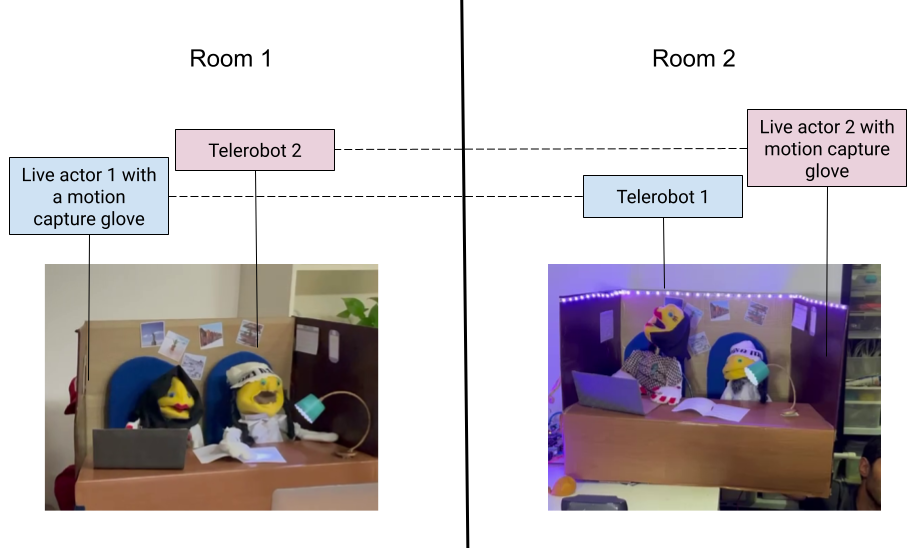
\includegraphics[width=1\linewidth]{Telerobotic puppetry.png}
    \caption{In participatory telerobotic puppetry, participants prepare two identical versions of a puppet theater and place them in separate locations. In each theater, one puppet is operated by a live actor and the other is a telerobot that mirrors the movements of the remote actor.}
    \label{fig:telerobotic_puppetry}
\end{figure}

We developed a kit (introduced in Article 3 \cite{peledTeleroboticTheaterOppressed2025}, see Figure \ref{fig:telepupetry-kit}) to be used in the workshop where participants could learn the technology and use it to create a telerobotic puppet theater. The participants use the kit and workshop materials to create two identical puppets, one is a regular glove puppet and the other a robotic puppet (see Figure \ref{fig:telepuppetry-diagram}). A participant performs with the regular puppet while wearing a motion capture glove (Rokoko smart glove\footnote{\url{https://www.rokoko.com/products/smartgloves}}), the glove transmits the movements wirelessly to a computer (with Touchdesigner software\footnote{\url{https://derivative.ca/}}) which processes the data and transmits robot actuation commands to the remote puppet (running on Raspberry Pi\footnote{\url{https://www.raspberrypi.com/}}). Through this process, the robotic puppet mirrors the movements of the glove puppet in real time. The voice of the performer is transmitted to the remote location via a standard voice call.

\begin{figure}
    \centering
    \includesvg[width=1\linewidth]{Telepuppetry diagram.svg}
    \caption{The flow of data in telerobotic puppetry, as shown in \cite{peledTeleroboticTheaterOppressed2025}. The live actor wears the glove puppet on a smart glove. Motion data is processed in Touchdesigner and transmitted to a Raspberry Pi that operates the pneumatic board.}
    \label{fig:telepuppetry-diagram}
\end{figure}

Telerobotic puppet actuation is based on the pneumatic textile design in the work of Cappello et al. on a soft robotic glove \cite{cappelloExploitingTextileMechanical2018,cappelloAssistingHandFunction2018}. The kit contains an engraved laser-cut panel for mounting the hardware components (pneumatic circuits and servomotors) with 3 printed housings (see Figure \ref{fig:telepupetry-kit}). Workshop participants are required to assemble the kit, configure the Touchdesigner project to read the desired fingers from the smart gloves, and configure the Raspberry Pi software with the appropriate PINs of their actuators. All software and hardware designs are released as open source in our Git repository, including documentation and tutorials. The kit was designed to allow maximum creative freedom for workshop participants - the pneumatic actuators are modular and can be attached to any fabric body. The production process demands collaboration between participants with basic knowledge of technology (to assemble the robot), participants with knowledge in sewing and crafting (to create the puppets), designers, and engineers. The aim was to create collaboration between participants with different skills and to introduce the technological aspect to everyone when all puppet components are integrated into one experience.     

\section{Field Study}
We conducted a field study of the concept with Israeli and Palestinian participants. Telerobotic TO has two distinct phases. In the first phase, participants from two conflicting groups meet in a participatory workshop and create a telerobotic puppet theater together, to be performed in the locations of both groups simultaneously using telerobotic technology. In the second phase, the theaters are set up in the two locations and performed publicly with live audiences. We conducted a field study that implemented the first phase, gaining insight into the entire process. During the workshop, the participants produced three puppet theater plays in three teams, each play was duplicated and tested across two rooms simulating Israel and Palestine.

According to the request of Tech2Peace, the workshop was limited to one weekend. Most of the time was spent creating the robotic theaters, leaving just enough for each team to premiere their play once (5 to 10 minutes). Therefore, we did not conduct theatrical interventions, iterations, and a discussion with the Joker and the audience, as in traditional Forum Theater. Instead, the focus was on the process in which the participants, who were neither theater nor engineering professionals, produced technological plays about the conflict. The weekend was framed as a follow-up activity for Tech2Peace alumni who completed their three-week seminar. Therefore, they already had experience in conflict resolution. The objective was not to determine whether the format can improve attitudes between the general populations of the groups, but to study the strengths and weaknesses of the concept as a medium for intergroup contact and to learn lessons for future facilitation of the workshop and its subsequent performances.

Data collected from the workshop included notes, videos, photos, and the scripts of the plays. We also held semi-structured group interviews with each team during the workshop and 10 interviews with individual participants after the workshop. The group discussions were free and moderated by the researchers only to ensure that all voices are heard. We asked the team about their current state and how they decided on the design, as well as general feedback on the concept and whether they imagine showing their play to an outside audience. The participants in the individual interviews were selected to include representatives from all teams and nationalities, with higher priority given to those who took on the role of performing with the telerobotic puppets. The interviews focused on the personal experience of the participants throughout the stages of the workshop. The analysis followed the practice of reflexive thematic analysis \cite{braunUsingThematicAnalysis2006,braunReflectingReflexiveThematic2019}. The unit of analysis was defined as a statement made by the participants, and the first author assigned the codes and themes to the transcribed interviews and the documented media. The codes were then reviewed by the second author. After multiple coding iterations, the data from all sources was triangulated \cite{guionTriangulationEstablishingValidity2011} and integrated into 4 themes: 1) Intergroup contact with puppets and technology, 2) Digital contact with telerobotics, 3) The role of humor and 4) Lessons for participatory design.

\begin{figure}
    \centering
    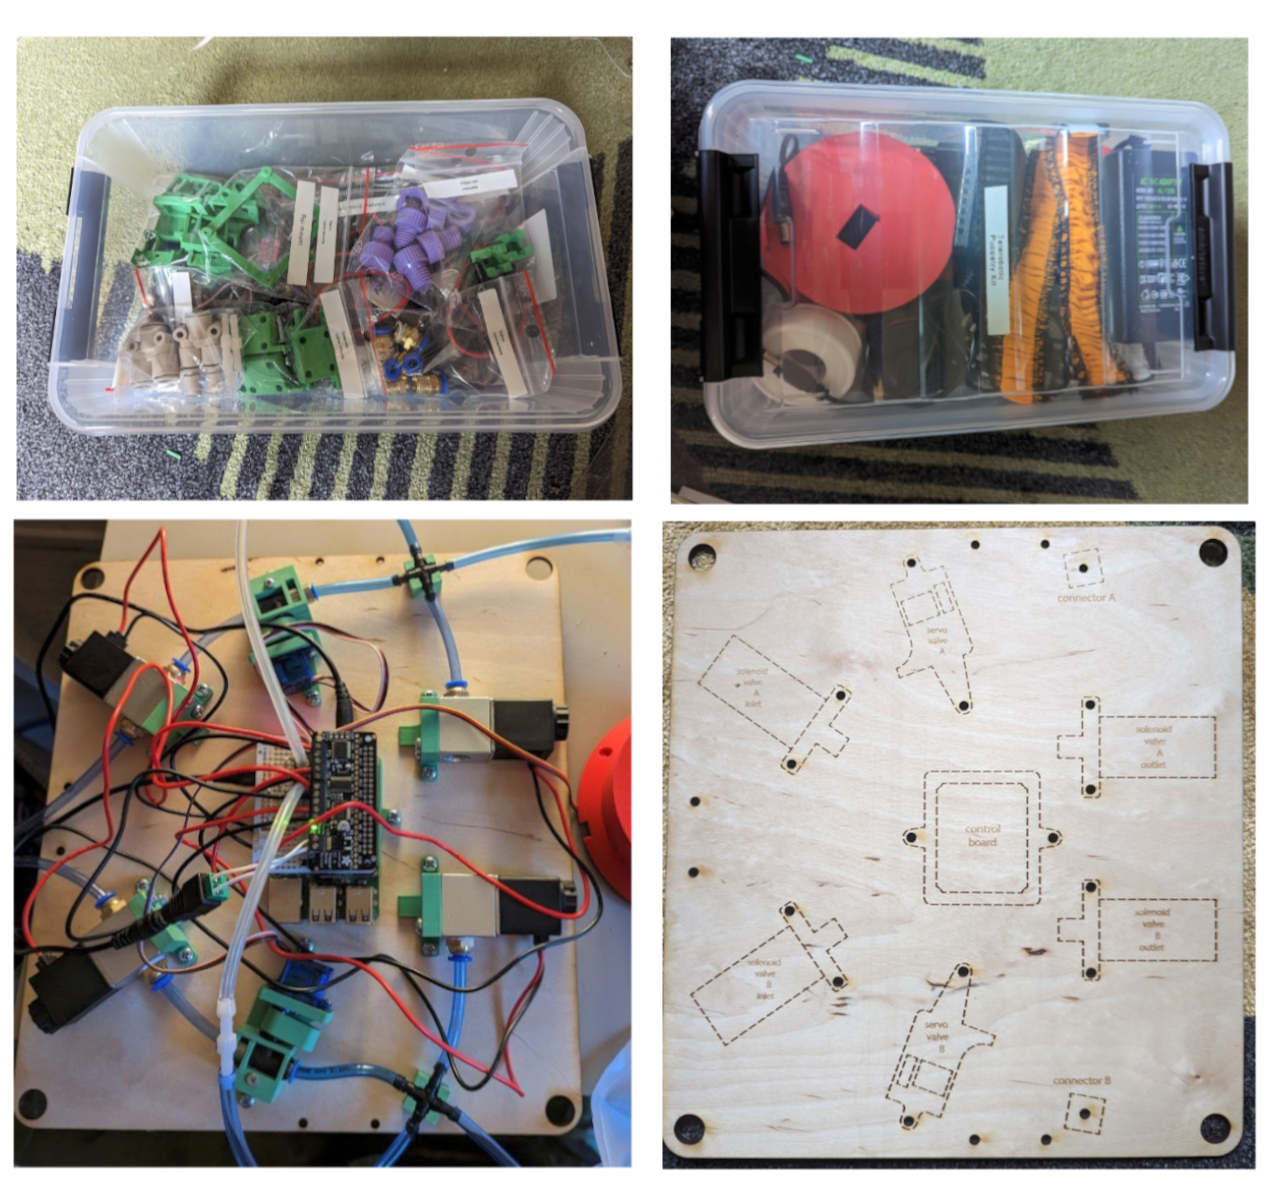
\includegraphics[width=1\linewidth]{puppetry-kit.png}
    \caption{The telerobotic puppetry kit as shown in \cite{peledTeleroboticTheaterOppressed2025}. Participants mount the Raspberry Pi, pneumatic valves, and servo motors on a provided engraved panel. Component housings are 3D printed.}
    \label{fig:telepupetry-kit}
\end{figure}

\chapter{Summary of the Articles}
\section{Article 1 - The Telerobot Contact Hypothesis}
The field of intergroup contact started with the contact hypothesis of Gordon Allport \cite{allportNaturePrejudice1954}, defining the conditions of contact that optimize the reduction of prejudice between social groups. In this article, we propose telerobots as a medium for intergroup contact and begin the study of \textbf{RQ1} by defining the hypotheses for their design and architecture. The premise was that telerobots are located in the middle ground between the physical and virtual realms, providing the flexibility of online communication and the depth of physical interactions. We combine research from intergroup contact theory, communication studies, and human-robot interaction to derive a conceptual model of how prejudice could be reduced in a telerobotic-based contact. We propose that the key determining factors are: previous attitudes toward robots, the sense of presence, and group salience. After which, we outline a set of guidelines and caveats in the following design aspects: system architecture (symmetric or asymmetric), telerobot appearance, the use of an embedded display, voice design, robot materiality, movement in space, verbal and nonverbal communication, teleoperation feedback, semi-autonomous functions, and operation in a public space. We end with recommendations and hope for further empirical research, stressing the importance of a transparent and participatory design process.

\section{Article 2 - Telerobotic intergroup contact: acceptance and preferences in Israel and Palestine}
Based on the results of Article 1, we continue the exploration of \textbf{RQ1} by conducting a survey on the acceptance and preferences of the telerobotic medium in Israel and Palestine. The survey explored the general acceptance of telerobotics as a casual communication tool and as a means to meet the outgroup. The survey also collected the preferences of the participants for telerobot appearance, its features, its representation of the operator, and the anonymity of the operator. Each of these aspects was explored for both a casual scenario and an outgroup scenario. We analyzed the responses using a mixed-method approach. The results showed that while Palestinians were generally less interested in meeting the outgroup than Israeli Jews, they preferred the telerobotic medium over other mediums. In contrast, Israeli Jews were deterred by the concept of telerobotics and preferred to meet the outgroup by video call or face-to-face. Both groups preferred a human appearance in both scenarios and having the interlocutors visible via a camera feed. Participants also preferred to represent their nationality via the telerobot when meeting the outgroup. Further analysis showed a greater need for Israeli Jews, the advantaged group, to avoid dehumanization, especially when the operator is visible. Finally, we saw potential in designing the telerobots as puppets, allowing participants to be themselves and a different identity simultaneously, supporting the 'dual identity' strategy for intergroup contact.

\section{Article 3 - Telerobotic Theater of the Oppressed in Israel and Palestine: Becoming Digital Jokers}
Based on the answers to \textbf{RQ1}, we developed the concept of participatory telerobotic puppetry. To answer \textbf{RQ2} and \textbf{RQ3}, we developed the telerobotic puppetry kit and hosted a workshop with Tech2Peace, an organization for technology education and dialogue in Israel and Palestine. Following the participatory theater method of Augusto Boal, The Theater of the Oppressed, participants, who did not have experience in theater, produced a puppet play about the Israeli-Palestinian conflict. Our addition to Boal's methods was that the theater was telerobotic, designed to run simultaneously on both sides of the separation wall. In a weekend workshop, participants learned to use the technology, created three plays, and performed them in two separate rooms that simulated Israel and Palestine. We analyzed qualitative data consisting of semi-structured interviews and documentation. The findings demonstrated how the concept promotes intergroup contact in two phases: first, through creative collaboration and dialogue over the design of the telerobotic theater, and second, through remote performances where the presence of the remote puppeteer is felt by the audience and co-actor. The analysis instructed us on adapting Boal's facilitation method, the joker system, to use and teach boundary-crossing technology as 'Digital Jokers'. We expanded the concept by proposing to include online mobile puppet operators and by highlighting the power of puppets and humor to ease the acceptance of intergroup contact with a more hawkish audience.  
% 
%. Results (e.g. 10-20 pages) 
%- Describe all the observations and insights you made during your research 
%- Present answers to your research questions 
\chapter{Results}

\section{Conceptualization of Participatory Telerobotic Puppetry (RQ1)}
This section outlines how the results of the conceptual review (article 1) and the user survey (article 2) answer \textbf{RQ1} and how these answers determined the conceptualization of participatory telerobotic puppetry.

\subsection{Telerobotic architecture}
The review hypothesized that a symmetric telerobotic architecture better supports Allport's condition of equal grounds, as opposed to an asymmetric architecture in which typically one side is "hiding" behind a robot and viewing their conversation partner through a camera \cite[p. 78]{peledTelerobotContactHypothesis2022}. This finding is especially relevant for asymmetric conflicts that are characterized by a power imbalance. This sentiment was reified in the survey findings \cite[p. 11]{peledTeleroboticIntergroupContact2024}: Although we did not explicitly describe to the participants the concepts of symmetric and asymmetric architectures, the majority of survey participants preferred to be seen through a video feed when operating their robot, as well as seeing their interlocutor (in both the casual and outgroup asymmetric scenarios). Within Israeli Jews, we saw a significant increase in maintaining anonymity in the outgroup scenario, but crucially, they preferred to apply anonymity to \textit{both} sides of the conversation. In addition to the sense of equality, a symmetric architecture was hypothesized to contribute to the sense of presence of both parties in the conversation compared to an asymmetric architecture \cite[p. 78]{peledTeleroboticIntergroupContact2024}. In asymmetric architectures, one side operates the robot remotely, and their sense of embodiment (referred to in the article as 'self-presence') is contingent upon the quality of the operation interface. The other side, on the other hand, is fully embodied, situated next to the telerobot, and their sense of co-presence depends on how well the presence of the operator is apparent in the robot. However, in a symmetric architecture, both sides are present locally - situated next to the partner telerobot, while the operation of their remote robot occurs transparently. Meaning, the movement and speech of the participants is detected while they interact with the partner robot and is transmitted to the other side where they are represented by their own robot.

The conceptual review also mentions possible benefits of asymmetric communication: insofar as the teleoperator perceives a disconnect between them and their robot, they could enjoy the benefits of CMC communication, such as managing the disclosure of identity, freedom of expression, and conformance to group identity over a personal one \cite[p. 78]{peledTelerobotContactHypothesis2022}. Significantly, analysis of the survey (which focused on asymmetric architectures) found that Palestinians appear to perceive the telerobotic scenario as less intimate than a video call or face-to-face and are therefore less concerned that it constitutes a normalization of relations \cite[p. 13]{peledTeleroboticIntergroupContact2024}. One participant who noted their concern of normalization and refused to communicate with Israeli Jews via video or face-to-face, favored the telerobotic option and added that they hope the meeting would be less 'resonating [\foreignlanguage{arabic}{صداه}]'. To preserve these benefits of asymmetric communication in which the operator is behind a mediating device, we suggest the puppet as a protective medium (see Figure \ref{fig:symmetric-telepuppetry}). The operator does not interact directly with the robot of the partner, but only through their puppet. This adds a layer of abstraction and representation.

\begin{figure}
    \centering
    \includesvg[width=1\linewidth]{Symmetric_Puppet.svg}
    \caption{Symmetric telerobotic puppet architecture: Each side of the conversation is locally present with their partner's telerobot, but the local puppet sets a boundary, creating a safer space for interacting with the outgroup.}
    \label{fig:symmetric-telepuppetry}
\end{figure}

The symmetric puppet theater architecture also solves several issues that the conceptual review found regarding the operation of the telerobot. The conceptual review notes the importance of nonverbal communication in intergroup contact \cite[p. 84]{peledTelerobotContactHypothesis2022}. For an engaging and more meaningful conversation, interlocutors should communicate emotions through expressive body language and facilitate turn-taking in the conversation with implicit signals such as gaze and body shifts. However, incorporating these signals in a symmetric telerobotic architecture requires elaborate detection of the interlocutor's body and fine-grained translation of the movement to the telerobot. Furthermore, the system should encourage the participants to use clear body gestures during the conversation so that they are easily transmitted to the robot. Designing the telerobotic architecture as a puppet theater rather than a standard face-to-face conversation significantly reduces the degrees of freedom that the system should process. First, through the use of glove puppets, body language is reduced to the use of the hand. Hand gestures are easier to pick up than whole-body gestures, and the history of puppet theater shows that it is possible to portray a range of emotions using a hand puppet. Second, the theater context forces the participants to use clear expressive language when puppeteering, ensuring the use of nonverbal communication with the robot.

Finally, the puppet theater architecture addresses the movement limitation introduced by a symmetric architecture. The conceptual review suggests that movement in space may be a desired feature of robots for intergroup contact \cite[p. 84]{peledTelerobotContactHypothesis2022}. First, because it highlights the advantage of robots over other digital communication methods - being situated in a physical space. Second, in conflict situations, such as the Israeli-Palestinian conflict, where movement of one group in the space of the other group is restricted, robotic movement could be an empowering factor. The survey confirmed that traveling in space was one of the top requested telerobot features in both groups and scenarios (although decreased for Israeli Jews in the outgroup, as we explain in terms of group differences). However, a symmetric architecture restricts the ability of the telerobot to move since the operator does not have a control interface. Movement is then available only through sensors that detect the movement of the operator in local space. The telerobotic theater architecture solves this because a puppet theater is a restricted space by design. Therefore, we can restrict the movement of the puppet to the confined borders of the theater without hindering the experience of the performer.

\subsection{Puppets, avatars, and dual identity}
The conceptual review and the survey explore options for representation and identification in a telerobotic avatar through the lens of intergroup contact. The multitude of previous research findings and possible design combinations make this topic convoluted. Therefore, in this section, I summarize what I consider the most important survey findings in Table \ref{tbl:avatars}, which I will juxtapose with the conceptual review. Following the discussion of the table, I will argue that the puppet theater architecture simplifies the dilemmas at hand. As we can see from the table, we explored two mutually exclusive dimensions for telerobot representation. The first is the appearance of the avatar. An avatar could appear human or nonhuman (such as a machine, animal, or caricature). When choosing a human avatar, operators could also decide how much it resembles them (for example, gender, age, religion, and nationality). The second dimension is that of anonymity. In the survey, we offer telerobot operators to be visible to their interlocutor through a camera feed placed on or near the robot. Therefore, even if the operator is not visually represented by the robot, they could still be identifiable.

\begin{table}
\caption{A matrix highlighting survey findings on telerobot identity with two distinct aspects: operator identifiability (via a camera video feed) and telerobot appearance (human/nonhuman and visual similarity to the operator).}
\label{tbl:avatars}
\definecolor{identColor}{RGB}{238,238,238}
\definecolor{anonColor}{RGB}{188,188,188}
\definecolor{humanColor}{RGB}{182, 207, 240}
\definecolor{nonhumanColor}{RGB}{255, 213, 173}
\definecolor{white}{RGB}{255, 255, 255}

{\small
\begin{tabular}{|m{4.5cm}|p{4.5cm}|p{4.5cm}|}
\hline
\begin{tabular}{@{}m{4.5cm}@{}} Telerobot appearance $\rightarrow$ \\ Operator identifiability $\downarrow$ \end{tabular} & 
\cellcolor{nonhumanColor}{Nonhuman / Not resembling to operator} &
\cellcolor{humanColor}{Human / Resembling to operator} \\
\hline

\cellcolor{identColor}{Identified (operator is visible via a video feed)} & 
\gradientcelltall{Most of the participants who wished to be 'someone else' through the robot still wanted to be seen through the video feed.}{identColor}{nonhumanColor} &
\gradientcelltall{• Most of the participants chose this combination. \\ • Preference to express nationality significantly increased for the outgroup scenario. \\ • Israeli Jews significantly switched their choice from machine to human for the outgroup scenario.}{identColor}{humanColor} \\
\hline

\cellcolor{anonColor}{Anonymous (operator is not visible)} & 
\gradientcelltall{Israeli Jews were significantly more likely to select a nonhuman appearance in the outgroup scenario when choosing to be anonymous.}{anonColor}{nonhumanColor} &
\gradientcelltall{}{anonColor}{humanColor} \\
\hline
\end{tabular}
}
\end{table}

As shown in the matrix, the survey found that a humanoid robot that also allows the operator to be seen through a camera was the most favorable option for interacting with the outgroup (for both groups) \cite[p. 11]{peledTeleroboticIntergroupContact2024}. The conceptual review hypothesized that a nonhuman avatar in the context of intergroup conflict may evoke a sense of dehumanization, which is a common perception between groups in an intractable conflict \cite[p. 79]{peledTelerobotContactHypothesis2022}. This hypothesis may explain why the preferred choice for a telerobot was a human. Furthermore, the survey found that Israeli Jews significantly changed their robot appearance from "machine" to "human" when faced with the outgroup scenario. The existence of this phenomenon only within Israeli Jews reflects the heightened need of the advantaged group to restore its moral image. The survey also found that both groups wanted to represent their nationality through the robot in the outgroup scenario, and decreased their preference to 'be someone else' \cite[p. 11]{peledTeleroboticIntergroupContact2024}.

However, our review also found advantages in using a nonhuman avatar, or one that does not resemble the operator \cite[p. 81]{peledTelerobotContactHypothesis2022}. A human avatar may appear uncanny or reduce the sense of agency of the operator, and resemblance to the operator may restrict their freedom of expression. Importantly, we found that of those participants who chose to try a "new identity" through their robot's appearance, the majority still wanted to be seen through the camera feed. We attribute this finding to the preference for equality and transparency when interacting with the outgroup. Consequently, we found that anonymity significantly increased the preference of Israeli Jews to select a nonhuman avatar,\cite[p. 11]{peledTeleroboticIntergroupContact2024}, signifying that the participants perceived a negative connotation of the nonhuman appearance and felt more comfortable selecting it when they are anonymous \cite[p. 4]{peledTeleroboticIntergroupContact2024}. We also found that the preference for anonymity increased in the outgroup scenario for both groups, but significantly only for Israeli Jews. Our conceptual review found that anonymity could promote self-disclosure, expression of group identity, and increase the intimacy of the conversation, but at the same time decrease the sense of social presence \cites[p. 78]{peledTelerobotContactHypothesis2022}[p. 4]{peledTeleroboticIntergroupContact2024}.

The conflicting advantages and disadvantages for robot appearance and identifiability encouraged us to change the basic paradigm regarding telerobotic communication. Instead of having the telerobot as an avatar that represents its operator, we regard it as a puppet that has its own identity and story. The puppet is not without a puppeteer, who can remain identifiable (at least by nationality) during the performance. In the conceptual review, we recommend against embedding a display in the puppet so that multiple dimensions are not conflated in the same object \cite[p. 81]{peledTelerobotContactHypothesis2022}. However, we recommend making use of the physical space around the robot to add additional identity cues \cite[p. 79]{peledTelerobotContactHypothesis2022}. When the puppet is not described as a representation of its puppeteer, its appearance can be varied without invoking the sense of dehumanization \cite[p. 88]{peledTelerobotContactHypothesis2022}. Furthermore, separating between puppet and puppeteer supports the use of a 'dual identity' strategy (and a 'metaxis'), in which the audience and the puppeteer can perceive the puppet under a separate, theatrical context, and the identity of the puppeteer simultaneously. Embedding intergroup contact in the context of a puppet theater also provides content for the encounter and supports the 'narrative' type of meeting, where participants can share their perspective on the conflict through storytelling and potentially expose a further audience to vicarious contact via a public performance \cite[p. 88]{peledTelerobotContactHypothesis2022}. Finally, the conceptual review recommends the use of soft materials for the design of the robot to support a nonviolent context \cite[p. 83]{peledTelerobotContactHypothesis2022}. The traditional fabric-based materiality of puppets is suitable for this purpose.

When we designed the survey, we had already considered the puppet theater format. Therefore, we included some questions to gather initial insight into the concept. The results showed less interest in a telerobotic puppetry scenario (both symmetric and asymmetric) than in a standard telerobotic avatar \cite[p. 10]{peledTeleroboticIntergroupContact2024}. However, a deeper inspection of the data revealed several findings that supported further research. Israeli Jews were collectively less inclined to use telerobotic communication in any scenario (perceiving it as 'strange') \cite[p. 8]{peledTeleroboticIntergroupContact2024}. However, for some participants who were deterred by telerobotics, the robotic puppet theater scenario was appealing \cite[p. 13]{peledTeleroboticIntergroupContact2024}. For Palestinian participants, although the puppet scenario was less appealing than the standard telerobotic scenario, it was still more favorable than a video call or a face-to-face meeting \cite[p. 10]{peledTelerobotContactHypothesis2022}. One Palestinian participant stood out as a perfect candidate for telerobotic puppetry \cite[p. 14]{peledTeleroboticIntergroupContact2024}. The participant initially displayed an antagonistic approach, marking 0 out of 100 as their sentiment toward Israeli Jews (0 denotes unfavorable) and selecting 'undecided' for using any medium of communication with them. However, when presented with the option of collaborating in a symmetric robotic puppet theater, chose 'definitely yes' and suggested the following story for the play:
\begin{displayquote}
The story is about a religious idea and how they occupied our land by force, robbed our
religious places, and many beliefs.
\end{displayquote}

The story suggested by this participant also reflects the difference in needs between the advantaged and disadvantaged groups when addressing the conflict. When asked about a possible storyline for a collaborative puppet play, most Israeli Jews avoided referencing the conflict and described more peaceful stories or plays for children \cite[p. 14]{peledTeleroboticIntergroupContact2024}. A similar theme was found in open questions about hopes and concerns and wishes for robot features for the outgroup scenario \cite[p. 13]{peledTeleroboticIntergroupContact2024}. Israeli Jews listed hopes for reconciliation, understanding, and general goodwill, while Palestinians suggested using the robot to explain about the conflict, for example:
\begin{displayquote}
Ability to speak the Hebrew language and to have information about the Palestinian
people and the suffering they endured from the Israelis.
\end{displayquote}
The recognition of the different needs of the groups and how the telerobotic encounter could be used for empowerment, as well as a multitude of opinions and strategies for telerobotic design, inspired us to use a more participatory approach for the solution, outlined in the next section.

\subsection{From customization to participation, learning and TO}
The conceptual review highlights the advantage of not only allowing users to customize the appearance of their robot, but inviting them to a process of co-design and co-creation \cite[p. 80]{peledTelerobotContactHypothesis2022}. The advantages found in the review include an increased sense of self-extension to a self-made telerobot and more positive attitudes from the users who participated in the design of their robot. In addition, in the context of intergroup conflict, therapeutic, educational, and empowerment aspects of participatory art were hypothesized to be positive contributors \cite[p. 80]{peledTelerobotContactHypothesis2022}. These benefits, in conjunction with the participatory frameworks of TO and participatory design, were put together into one format (outlined in the field study article \cite{peledTeleroboticTheaterOppressed2025}). Israeli Jews and Palestinians would design telerobotic puppets together and learn about technology. As in Forum Theater, participants would discuss their views about the conflict in theater plays, despite not having any previous experience in the performance arts.

The educational path also proved useful in the task of finding an NGO that would collaborate with us on the project. The Tech2Peace organization \footnote{\url{https://www.tech2peace.com/}} holds joint seminars with Israeli Jews and Palestinians that combine technological education and dialogue. We approached Tech2Peace, and they invited us to conduct a weekend seminar with alumni from their main three-week seminar. The results are described in the following section, detailing the results of the field study.

\section{Concept evaluation (RQ2)}
The results of the conceptual review and survey answer the research question: How could telerobotics be integrated as a medium of intergroup contact in the form of a participatory telerobotic puppet theater? The field study conducted with Israeli Jews and Palestinians in Tel Aviv evaluated the answer to this question with empirical data and provided further insights for future implementations. In the analysis, we termed the role of the facilitator as a 'digital Joker', referring to Boal's TO facilitator, the Joker. Therefore, I divide the findings into two sections: 1) Concept evaluation and 2) Facilitation guidelines for digital jokers.

The findings of the study showed how the telerobotic theater creation process promoted intergroup contact and dialogue (Theme 1: Intergroup contact through puppets and technology \cite[p. 14]{peledTeleroboticTheaterOppressed2025}). Firstly, through collaborative work \cite[p. 14]{peledTeleroboticTheaterOppressed2025}: Participants reported creating friendships and bonds, not just through the co-design of the technology, but also through the traditional puppet crafting tasks. However, technology was the main driver of the participants for the workshop, and the concept of a cross-border telerobotic performance sparked discussions within the groups (I elaborate on that in the next section on facilitation). We also found that Large Language Model (LLM) technology helped some of the groups resolve disagreements and dilemmas \cite[p. 22]{peledTeleroboticTheaterOppressed2025}. Secondly, we found that the puppets were a liberating tool to talk about the conflict \cite[p. 13]{peledTeleroboticTheaterOppressed2025}: The participants from both groups agreed that it was easier for them to talk about the conflict through puppets and that it makes the conflict more accessible to an audience, for example:
\begin{displayquote}
    \textbf{Participant 3 (PS):} It makes talking about the conflict - since it's a heavy topic or a sensitive topic, it makes it "Yeah! Let's talk!". Like the puppet is saying it -  it's not me.
\end{displayquote}
Third, by invoking dialogue as part of the theater design process: In the production process, participants raised questions about visual stereotypes, debated the aggressiveness of Israel in the control of water sources, discussed the debate around the origin of the 'falafel' dish, and made a statement for diversity by including a Muslim woman expert in AI in one of the plays \cite[p. 14]{peledTeleroboticTheaterOppressed2025}.

The findings also revealed the potential for digital intergroup contact between puppeteers located in different locations (Theme 2: Digital contact with telerobotics \cite[p. 16]{peledTeleroboticTheaterOppressed2025}. When performing the telerobotic play in two separate rooms, the puppet operators reported sensing the presence of the second puppeteer as if they were with them in the room. As common in traditional puppetry, the performers were hiding behind the set, relying on auditory feedback, not seeing the full stage or the audience (both local and remote). However, participants reported that while they were focusing on the performance, they felt that the second puppeteer was "sitting next to [them] and moving his own puppet" \cite[p. 16]{peledTeleroboticTheaterOppressed2025}. Therefore, they experienced co-presence with the remote puppeteer without experiencing telepresence of the remote environment. In this experiment, we did not test the sense of co-presence between the audience and the remote puppeteer. Nevertheless, insofar as the telerobotic puppet is not qualitatively different from the live puppet from the audience's perspective, the results could be extrapolated to show potential in that aspect. Furthermore, participants suggested adding a live video feed of the remote audience in each location, creating a sense of shared presence between the two audiences \cite[p. 16]{peledTeleroboticTheaterOppressed2025}.

Finally, the findings showed the potential for the concept to be accepted by Palestinians who oppose normalization of relations with Israeli Jews. Significantly, this was made possible through the use of humor in puppet plays (Theme 3: The role of humor \cite[p. 17]{peledTeleroboticTheaterOppressed2025}). Finding the balance between humor and a meaningful discussion of the conflict was a recurring topic of discussion in the groups. Eventually, two of the three groups chose a more humorous and satirical script for their play. The scripts also offered humorous commentary on technology \cite[p. 12]{peledTeleroboticTheaterOppressed2025}: One group took a naive reconciliation script made by ChatGPT and turned it into a satire, and another group joked about using ChatGPT to find the solution to the Israeli-Palestinian conflict. In a discussion about normalization, Palestinian participants, who were previously doubtful of the concept being accepted in Palestine, expressed the possibility of it passing through the use of humor:
\begin{displayquote}
\textbf{Participant 3 (PS):} It will, like, break and take that intensive feeling... if you use fun or jokes in the context. 

\textbf{Participant 2 (PS):} Yeah, I agree. It's black humor.
\end{displayquote}
This is joined by the previous finding of the study about the ease of talking about the conflict with puppets as well as by the findings of the survey that show that telerobotics could be perceived as a less 'resonating' form or normalization, all together painting a promising picture for the use of the concept in asymmetric conflicts.


\section{Facilitation Guidelines for Digital Jokers (RQ3)}
In the Discussion section of the field study article, we coin the phrase 'Digital Joker' (\cite[p. 19]{peledTeleroboticTheaterOppressed2025}. As mentioned in the Research Design chapter, the field study did not explore the traditional dramaturgical role of the Joker, such as facilitating discussion through theater and promoting audience participation (although these roles could certainly be assigned to the same facilitator). We defined the role of a Digital Joker as navigating participants through technology and facilitating the crossing of boundaries in a technological environment \cite[p. 19]{peledTeleroboticTheaterOppressed2025}. In fact, the role of the Digital Joker (much like the original Joker) revolves around the crossing of boundaries, but in the technological realm. I divide this section into two, in accordance with the two phases of the process: Boundary-crossing in the making phase and boundary-crossing during the performance.


\subsection{Boundary-crossing in the making phase}
\begin{description}
   \item[Between user and developer] If the TO Joker facilitates the transformation of a spectator to an actor, in the technological realm the Joker transforms the user to a developer. We found that this was particularly important in the context of intergroup conflict, because the NGO and the participants were motivated to join the workshop to gain new technological skills \cite[p. 19]{peledTeleroboticTheaterOppressed2025}. Inspired by TO, this transformation could be playful, iterative, expressive, and based on mutual learning. We also learned that it is important to understand the learning expectations of the participants beforehand to allow them to step out of their comfort zone \cite[p. 18]{peledTeleroboticTheaterOppressed2025}. Some participants were forced to use their strong skill (such as crafting) so that the team would meet the deadline to produce their play.
   \item[Between realms of content] In some cases, participants enjoyed using their existing professional and hobby skills, but in a completely new and artistic realm of content \cite[p. 18]{peledTeleroboticTheaterOppressed2025}. This was an emerging advantage of facilitating a multidisciplinary workshop, such as a telerobotic puppet theater, to participants who were outside both fields. For example, a civil engineer advised on the construction of the theater set, a mechanical engineer on the pneumatic robotic mechanism, and those with experience in sewing cloths learned to make puppets. Because the participants had a fresh perspective, they suggested original ideas for technology that would not have come up in a more traditional pedagogical context \cite[p. 18]{peledTeleroboticTheaterOppressed2025}. We saw the role of the facilitator as understanding the various skills of the participants and offering them suitable challenges in the technological realm.
   \item[Between gender roles] The nature of the concept, which combines textile work and mechanical engineering, could result in roles assigned according to gender, even to the dismay of the participants \cite[p. 19]{peledTeleroboticTheaterOppressed2025}. We saw the role of the digital joker as twofold: First, to ensure that gender roles are not assigned against the will of the participants. And second, to encourage the crossing of this boundary by suggesting engineering tasks to women and textile crafting tasks to men.
   \item[Between intergroup perspectives] The telerobotic aspect of the theater required the participants to think beyond their local perspective when producing the play, because of its capacity to reach cross-border audiences \cite[p. 15]{peledTeleroboticTheaterOppressed2025}. Participants discussed how their play and the presence of an actor from the outgroup would be regarded in their local region, and vice versa, how their presence would be regarded in the region of the outgroup. In this way, the Digital Joker facilitates a discussion on the difference in perspectives on the conflicts between the groups, and encourages the participants to find artistic methods (such as black humor) to make their play acceptable in a sensitive context.
\end{description}
\subsection{Boundary-crossing during the performance}
\begin{description}
   \item[Between intergroup spaces and identities] Following up on the discussion of acceptance, the participants suggested ways to ease the delivery of the intergroup context \cite[p. 16]{peledTeleroboticTheaterOppressed2025}. Multiple participants suggested that the identities and original locations of the remote puppeteers could be exposed only at the end of the play (the same could be applied to exposing the remote audience through video). We ascribe the role of discussing and managing the exposure of identities during the performance to Digital Joker. With the help of the technology, the Joker is faced with the challenge of maintaining the balance between acceptance and contact. As with TO, the technology could be delivered to the audience in a transparent and critical manner, mediating its inner workings to the spectators. Moreover, the Digital Joker could invite the participation of the audience to use the technology, join the telerobotic theater, and converse with the remote actors.
   \item[Between theater and world] In the Discussion section of the paper, we further expand the notion of audience participation brought up by the participants, suggesting inviting external puppeteers to the play using their mobile devices \cite[p. 20]{peledTeleroboticTheaterOppressed2025} (see Figure \ref{fig:telerobotic-to}). We borrow Boal's use of the Greek tragedy format in the Joker system \cite[p. 160]{boalTheatreOppressed2008}, where apart from the protagonist (in our version, there are two protagonists, one for each group), there are two choruses: deuteragonist and antagonist. Each chorus has a varying number of actors that play a role in support or against the protagonist. In this case, the Digital Joker would also orchestrate the participation of online actors during the performance. However, we recognize that this form of telerobotic operation, albeit provides access to virtually anyone to join the performance, breaks the symmetric architecture since the chorus operators are hidden behind their mobile devices \cite[p. 20]{peledTeleroboticTheaterOppressed2025}. We had a first opportunity to explore this format in the follow-up intervention, described in the next section.
\end{description}


\begin{figure}
    \centering
    \includesvg[width=1\linewidth]{Telerobotic-TO.svg}
    \caption{An illustration for a telerobotic TO as shown in \cite{peledTeleroboticTheaterOppressed2025}. The setup includes two symmetrical stages where each stage includes a hand-operated puppet, a telerobotic puppet, two mobile choruses operated by online mobile connections, a Digital Joker as the facilitator, and an audience.}
    \label{fig:telerobotic-to}
\end{figure}

\section{Follow-up intervention: Telebibi}
The following section is a recount of an intervention that I initiated in collaboration with participants of the Tech2Peace workshop, dubbed "Telebibi". The project was started as a response to the war that broke on 7 October 2023. Although the notes presented here were not processed as research data, I see them as essential to the discussion of the results of this thesis and of possible further research.
\subsection{Conception in response to October 7, 2023}
The field study with Tech2Peace took place on June 1, 2003, just four months before the start of the war. In the months following the workshop, I kept in touch with the participants (and mentors) through a WhatsApp group, updating them on the research progress and planning the next phase, which was meant to be the public performance of a theater in Israel and Palestine. After the events of October 7 in Israel and the ensuing assault on Gaza, it was clear that this would now be difficult to organize. Passages to and from the West Bank were closed, and both Israelis and Palestinians were dealing with their local grief. The WhatsApp group went silent, apart from a support message from Jan-Hinrich, our German collaborator, to which I and another Israeli participant replied, and others responded only with emojis. However, it was clear to me that I needed to do my part through this research. As the voices in Israel against the continuation of the war increased, I decided to try and create a local intervention. I contacted another Israeli participant of the workshop, Gal Gorfung, who was working on his own ideas for a workshop about AI content generation with cloned voices. I suggested that we try to follow up on the telerobotic workshop with an ad hoc theater. Inspired by the humorous and satirical content of the previous workshop and by Gal's work on voice cloning, we decided to build puppets in the form of political leaders and allow anyone from anywhere to connect using their mobile device and sound their voice through the voice of our leaders.

It was clear to me that the first puppet would be Benjamin Netanyahu, the prime minister of Israel. We managed to draft the other Israeli mentors from the workshop for the project and by the summer of 2024 we had a working prototype (see Figure \ref{fig:telebibi-making}). Ivan, the engineering mentor, decided to create a new and simpler robotic skeleton that could be 3D printed and does not use pneumatics. Marian, the art and design mentor, created the head of Netanyahu with felting, I created the new mobile app, and Gal coordinated the production. The operation app shows a 3D scanned model of the puppet on a virtual background. The app allows users to move the neck of the robotic puppet by moving the phone up or down and change its orientation by moving the phone left and right. Tapping the virtual button on the puppet makes it open and close its arms, and tapping the microphone button lets the users speak, which will be sounded through the puppet with the cloned voice of the character. All the instructions and code for 3D printing and building a puppet from scratch were published on our website which we named Forum Theater Online\footnote{\url{https://forumtheatre.online/}}.

\begin{figure}
    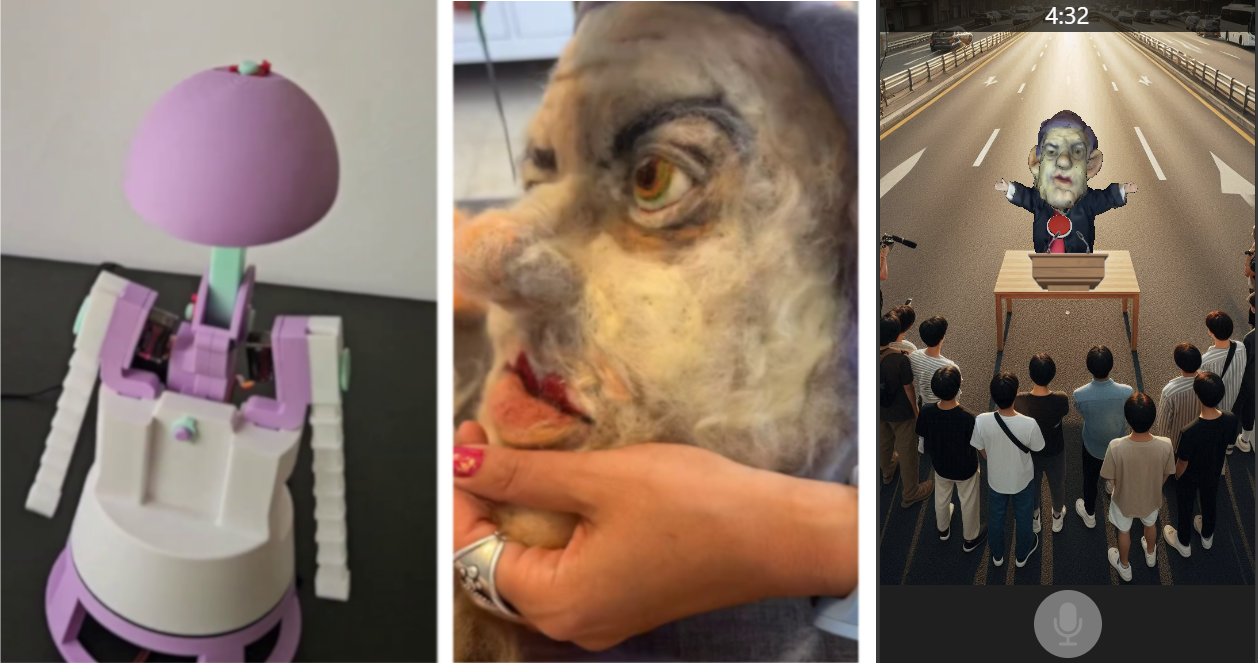
\includegraphics[width=1\linewidth]{telebibi-making.png}
    \caption{The components of Telebibi. From to left to right: The 3D printed robot by Ivan Lukomskiy, the head of the puppet by Marian Boo, and the operation app by Avner Peled.}
    \label{fig:telebibi-making}
\end{figure}

\subsection{Pilot}
The pilot of the project was held on August 24, 2024, in a weekly demonstration against the war in Tel Aviv (see Figure \ref{fig:telebibi-pilot}). We published the link to operate the puppet on social networks and in the WhatsApp group of the Tech2Peace workshop. We also had a QR code and explained instructions on-site for those attending the demonstration. Because only one user could operate the puppet at any moment, we set a limit of about 5 minutes (we varied the time in accordance with traffic) for every user and displayed a countdown queue to other users. The puppet received positive feedback from attendees of the demonstration and also attracted the attention of media reporters that were on the spot, eventually reaching several cable news outlets around the world. However, we did not see much traffic from people who were not present at the demonstration, possibly because they were overshadowed by on-site users and could not resolve technical issues without local guidance. Documentation from the event shows that passersby used the puppet in two ways: 1) satirical or cynical content that makes fun of the prime minister and 2) saying with the voice of the prime minister what they think he should say but does not. A video posted on German news 'Deutsche Welle' \footnote{\url{https://x.com/dwnews/status/1828640177465458992}} features an interview with one participant who describes their perspective on the project:
\begin{displayquote}
    I think it's a funny project, because it lets us [say] what we think that the Prime Minister Netanyahu should say, but he doesn't say.
\end{displayquote}
In an example of this, one participant had the puppet say that it announces its resignation and accepts responsibility for the events that happened on October 7.


\begin{figure}
    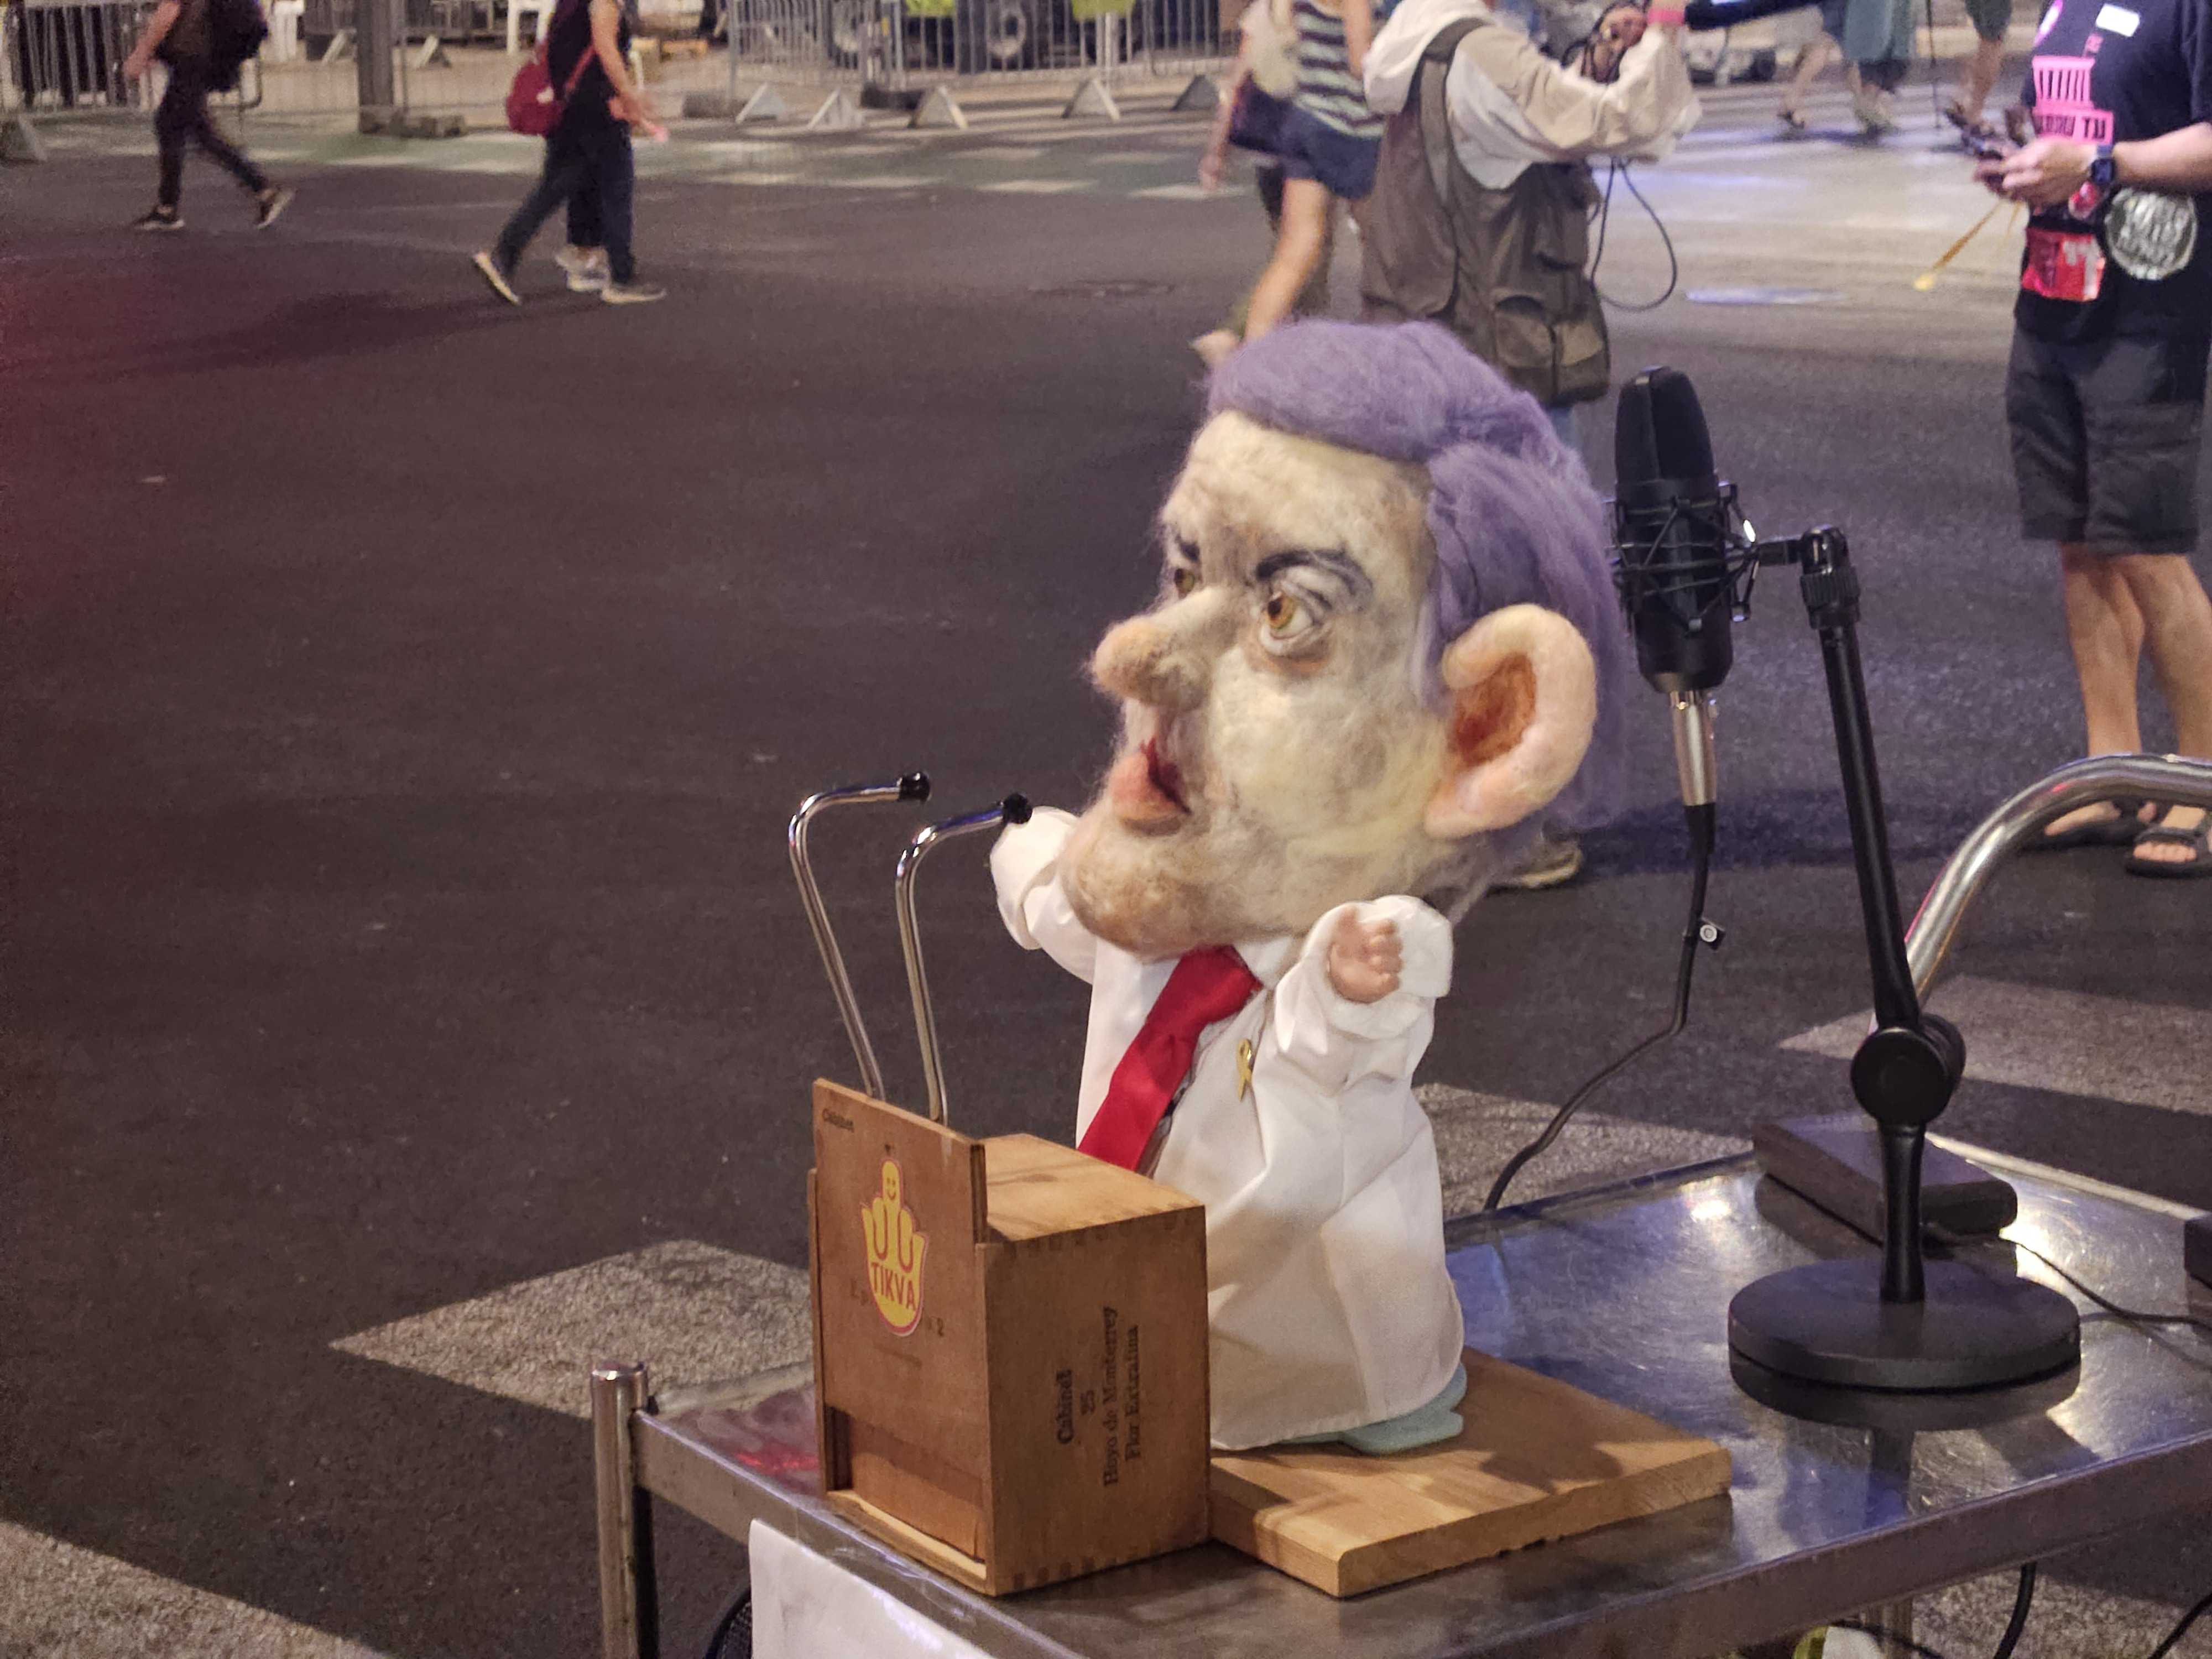
\includegraphics[width=1\linewidth]{telebibi.jpg}
    \caption{The Telebibi puppet attending a demonstration in Tel Aviv, Israel. Photo: Ivan Lukomskiy.}
    \label{fig:telebibi-pilot}
\end{figure}

%6. Discussion (e.g. 3 -6 pages) 
%- Get back to your research objectives and theoretical background / literature review 
%- Explain how your research related to earlier research 
%- Evaluate your results and compare them to what is already known 
%- Present the limitations of your research 
%- Understand the limitation of your research
\chapter{Discussion}

\section{Research contribution following the Matrix}
The \hyperref[sec:matrix_of_intersections]{matrix of field intersections} provides an overview of this research and its theoretical background. With the help of the matrix, we can reflect on the contribution of this thesis and devise a plan for future research. Starting with the title of this thesis and throughout its chapters, I have emphasized that the theory of intergroup contact is the theoretical foundation for the work. Therefore, it is appropriate to go by the first row of the matrix, which describes the dissolution of four fields in the field of intergroup contact, as a starting point. Then, I will consider each cell in that row and expand into further cells of the matrix to fully describe the contribution.

\subsection{Intergroup contact and PD}
There is a clear gap in the intersection of intergroup contact and PD - a need for participatory research where the participants design contact interventions that make use of technology. Contact research, let alone digital contact research, is still dominated by quantitative methods that require careful design of the scenario by the researchers. However, as noted in the review, there is a dire need to restore the community's agency in the design of the contact and correspondingly adjust research methods to a more open and qualitative nature \cite{dixonNegativeContactCollective2021}. At the same time, there is a call for PD researchers to collaborate with peacebuilding efforts \cite{bodkerAfterthoughtsEmergentFuture2025}. This thesis answers both of these calls in the form of a participatory telerobotic theater workshop. 

We have shown how incorporating technological education motivated participants to join the workshop and how the design of the technology and the theater promoted dialogue and the sharing of narratives - a favorable form of contact (especially in asymmetric conflicts). We have also shown preliminary results of how the participatory process persisted and pivoted in response to the political events with the Telebibi project. Although it did not yet expand to intergroup contact, the participants and mentors of the workshop were able to take the reins and drive the project forward to its new evolution. Considering the importance of length in both PD and intergroup contact, the natural path forward would be to plan programs that follow a similar line but aim for the long term. Long-lasting and gradual interventions would become critical when we expand the research to communities that have no previous experience in contact, as opposed to the field study which was conducted with alumni of the Tech2Peace program.

\subsection{Intergroup contact and Technological TO}
The integration of TO with intergroup contact, although rare, was explored in at least two previous research projects (polarized forum theater \cite{alonCHAPTERFOURTEENNonViolent2011} and forum theater for reconciliation \cite{miramontiForumTheatreReconciliation2025}). However, these projects did not use the intergroup contact framework, suggesting that there is room for more explicit use of this integration, exploring storytelling-based contact through TO and its influence on collective action, intergroup attitudes, and expanding contact through public TO performances. However, the primary contribution of this thesis is the use of technological TO (through PD) with intergroup contact. This combination is what gave birth to the concept of the Digital Joker. Although robots were previously used with TO and PD, they were not applied to facilitate contact and border crossing.

We have shown how the pedagogical, playful, and exhortative methods of TO and the Joker system could be applied to the education of technology in participatory design. We have also shown how the co-design of technology could be a part of the design of a theater, guided by the goal of intergroup contact and political expression. Crucially, we have expanded TO across spatial boundaries using telerobotic technology and augmented the role of the Joker with technology to facilitate cross-border participation. The findings of the field study and the follow-up intervention serve as a proof of concept and a technological prototype for this integration. The telerobotic puppetry kit uses glove puppets for a symmetric theater and the Telebibi project enables a more ad hoc use with mobile devices. However, the implementations in this thesis only scratch the surface of Boal's methods of liberation from oppression. I will expand on this further in the later section: Technology of the Oppressed Trickster. 

Finally, this thesis unveils a link between the thought of Brecht and Boal against the overuse of empathy in the theater, which counters the goal social change and current issues with intergroup contact that focuses on benevolence and empathy without driving for collective action. We can imagine what Brecht would say about the contemporary VR experience that offers participants the opportunity to take the perspective of the minority. Such experiences touch the emotion of the viewer, but it is doubtful that they promote meticulous and mundane action against institutional injustices. Future research could examine the relationship between Epic Theater and intergroup contact more closely.

\subsection{Intergroup contact and Telerobotics}
Starting with our initial 'Telerobot Contact Hypothesis', this thesis is the first to propose facilitating intergroup contact with telerobotic technology. The spatially segregated nature of the Israeli-Palestinian conflict demanded a solution that can, on the one hand, bypass physical restrictions and, on the other hand, maintain a connection to the disputed land. Telerobotics provides such a solution. The first two articles in this thesis combine previous research and an empirical survey in Israel and Palestine to determine the optimal strategy for integrating telerobotics into intergroup contact. We introduce a novel symmetric architecture that maintains the principle of equality and reduces the operation of the robot to hand movement detection, since we are operating a glove puppet. Although robots have been used in theater for entertainment, education, and HRI research, this is the first implementation in an intergroup context. 

The results show how the symmetric theater architecture promotes the sense of co-presence between the distanced puppeteers, a quality that was shown to improve digital contact encounters. Future research should explore the sense of co-presence between the distanced audience and between the audience and the remote puppeteers. I also present a prototype for asymmetric control from a mobile device using a 3D printed puppet and voice cloning. As proposed in the field study article, it is also possible to combine both architectures in one play.

The survey, for the most part, dealt with the more traditional asymmetric scenario of a telerobot being operated on a mobile device. However, we used the acceptance and preference results to design the telerobotic puppetry workshop. In particular importance to protracted and asymmetric conflicts such as the Israeli-Palestinian conflict, the survey found that the telerobotic architecture appears less resonating, more accessible, and a potentially empowering form of contact for the disadvantaged group. Although these results regarded the traditional telerobotic scenario, we found support for this in the field study, when combined with the qualities of humor and puppetry. 

The various preferences and connotations regarding telerobot appearance and operator identifiability, the support in the literature for robot co-design, as well as the differences found between the needs of the advantaged and disadvantaged groups, were addressed by separating between operator and puppet identity and granting design agency to the participants (and the Digital Joker). The format allows the participants to decide on the appearance of the telerobotic puppets and to manage the visibility of the operators during the play (for example, displaying them at the end of the play, with a digital accessory on the set). The last section outlines the contribution through the specific integration of intergroup contact and puppetry.

\subsection{Intergroup contact and Puppetry}
Puppetry was previously applied in intergroup contact as a pedagogical tool for an imagined contact with the outgroup \cite{charalampidouInventingNewRoad2022}, and in "applied puppetry" puppets were used in intergroup settings and areas of conflict \cite{grantObjectsObjectivesApplied2020}. However, this thesis is the first to use puppetry within the framework of intergroup contact to an encounter between the groups that is not imagined. More specifically, this thesis is the first to propose the application of the 'Dual Identity' strategy of Gaertner and Dovido to the 'double vision' aspect of puppets (which was previously applied also to Boal's Metaxis). Future research could focus more explicitly on this comparison, applying methods from the Dual Identity strategy in a puppet theater format, and examining the effect on collective action.

Our findings also affirm the therapeutic power of puppets in discussing sensitive topics such as the Israeli-Palestinian conflict. In fact, almost the exact same words were used by a Palestinian participant in the field study workshop and by Grant in his impression of the puppetry workshop in Belfast \cite{grantObjectsObjectivesApplied2020}: the puppet is saying it, not me. Furthermore, the concept of "radical empathy" through puppetry, a type of empathy that could be accepted as valid by Brecht and Boal, appears as a 'holy grail' for driving collective action in intergroup contact, reifying the need to perform further research on intergroup contact through puppets.

\section{Technology of the Oppressed Trickster}
A recurring theme in this thesis is that of boundary-crossing. Between research fields - art and science, engineering and social sciences, robotics and theater. Or in the process of a telerobotic theater of the oppressed, between spectator and actor, puppeteer and puppet, user and developer, researcher and participant, gender roles in science, engineering in arts. And finally, between physical and social borders, across the Israeli-Palestinian separation barrier, and between group identities and narratives in conflict. I see this urge to cross boundaries as a response to the state of stagnation and oppression brought about by protracted, intractable conflicts. Bar-Tal calls for a multidisciplinary approach against propaganda, and of creating cognitive contradictions to invoke an 'unfreezing effect' \cite{bar-talDanielBartalIsraelipalestinian2024}. Boal recognizes the need to be in the in-between, liminal space, where normal rules and constraints do not apply, to free ourselves from oppression. 

There is a mischievous element in boundary-crossing: it creates disorder. Combining many research fields and methods into one thesis makes it difficult for journal editors and peer reviewers to evaluate the work. Asking a mechanical engineer to sew puppets may spark some resentment. Situating a live Palestinian actor through a robot in Israel, and vice versa, or speaking with the cloned voice of the prime minister, may invoke a lot of resentment. But this mischievousness is not driven by malicious intent. It is the creation of disorder to break out of a 'local minima'; a frantic reaction to stagnation. 

This is also the intent of mythological tricksters. The trickster is an archetype for a character that appears in historical folklore and religious stories from multiple cultures \cite{hydeTricksterMakesThis2017}. The tricksters are known as playful boundary-crossers with divine powers such as shape-shifting and traveling between heaven and earth. Although they use their powers to create mischief, it is often for the benefit of humans \cite{hydeTricksterMakesThis1997}. Examples of tricksters are Hermes in Greek mythology, Coyote in Native American mythology, Eshu in the Yoruba mythology of West Africa, and Loki in Norse mythology. Lewis Hyde writes in the book "Trickster Makes this World":
\begin{displayquote}
Where someone’s sense of honorable behavior has left him unable to act, trickster will appear to suggest an amoral action, something right/wrong that will get life going again. Trickster is the mythic embodiment of ambiguity and ambivalence, doubleness and duplicity, contradiction and paradox... The boundary is where he will be found, sometimes drawing the line, sometimes crossing it, sometimes erasing or moving it, but always there, the god of the threshold in all its forms.
\end{displayquote}
The archetype example of a boundary-crosser is Eshu, the trickster god of the crossroads of the Yoruba people in West Africa \cite[ch. 5]{hydeTricksterMakesThis2017} (see Figure \ref{fig:eshu}). Eshu is described as the mediator between heaven and earth, as well as a troublemaker. When humans lost their faith in the gods and the gods lost their vital sacrifice from humans, Eshu used trickery to restore this relationship. He created a system of divination, which he obtained from the gods through guile, persuaded the humans to pay a sacrifice for the divine information, and ensured himself a cut of the profit. However, Eshu himself intervenes in the stories of the Yoruba diviners. His role is to introduce an element of chance and uncertainty to fate, and through that, to the rigid social status system of the Yoruba society. 

\begin{figure}
    \centering
    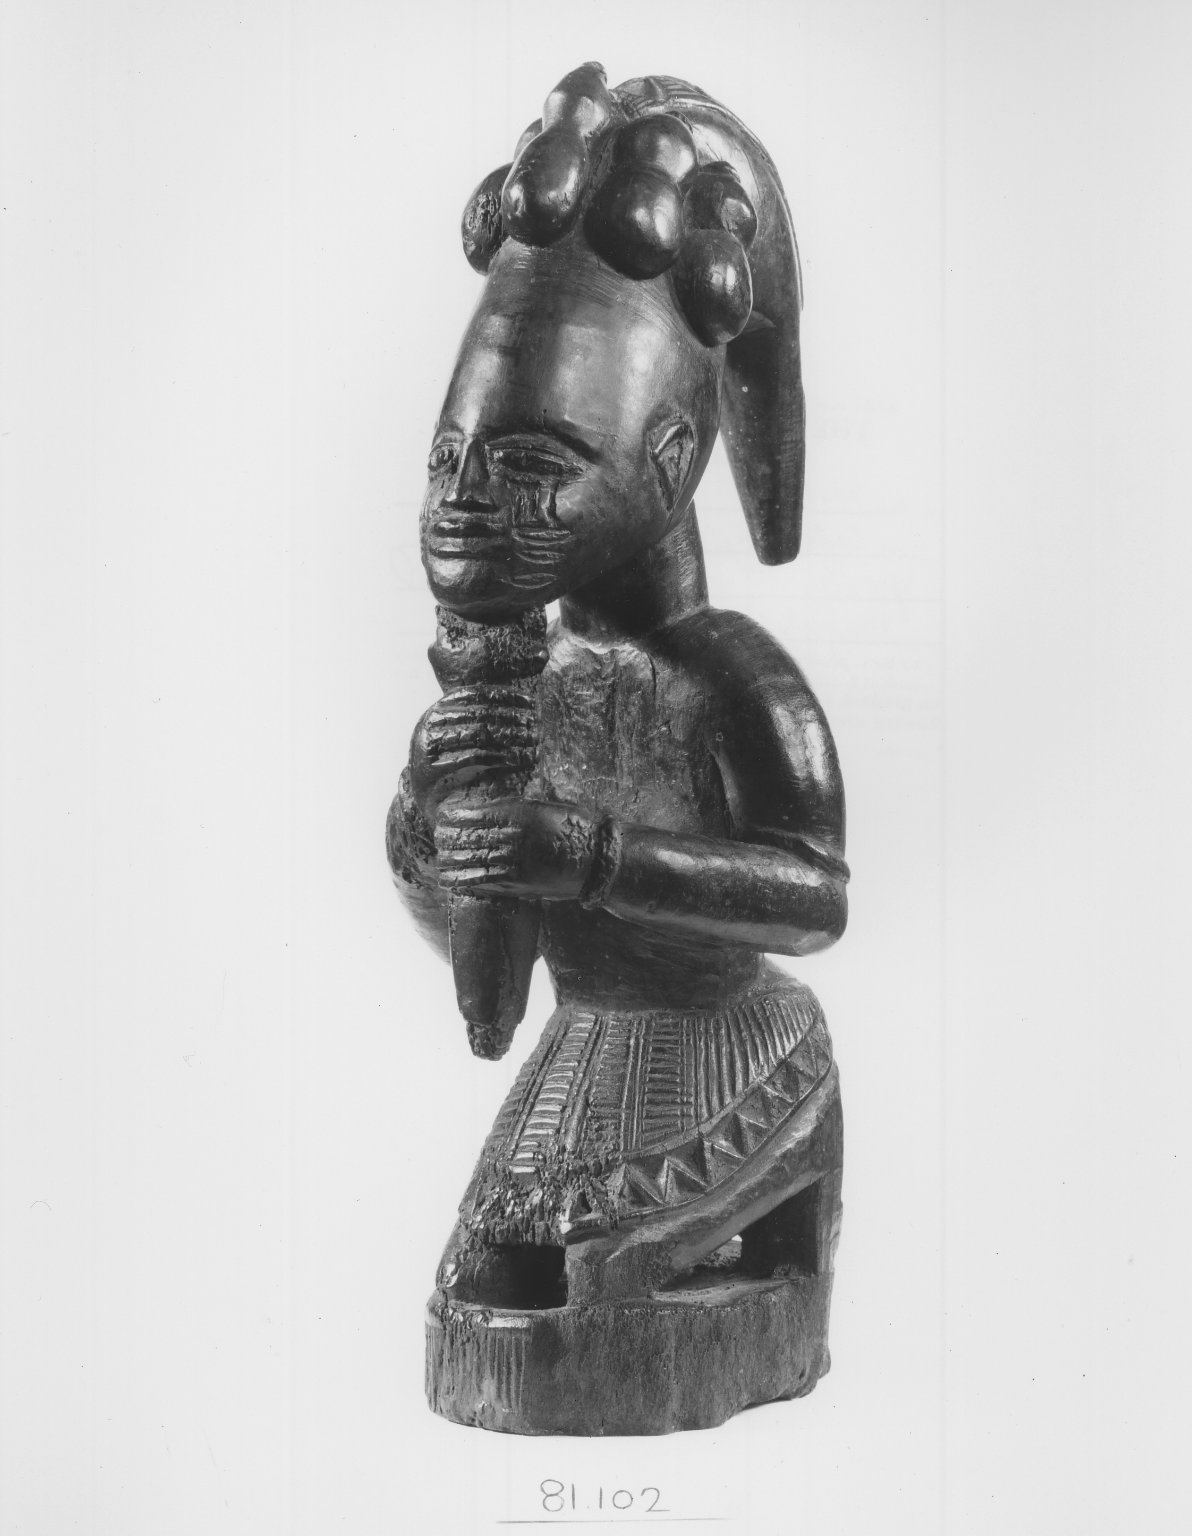
\includegraphics[width=0.5\linewidth]{eshu.jpeg}
    \caption{Kneeling Figure of Eshu-Elegba: the trickster god at the crossroad of the Yoruba people, Brooklyn Museum 81.102. From: \url{https://commons.wikimedia.org/wiki/File:Brooklyn_Museum_81.102_Kneeling_Figure_Eshu-Elegba_(3).jpg}}
    \label{fig:eshu}
\end{figure}

Mady Schutzman draws the line between the trickster and Boal's Joker. Referring to the original Joker system where actors switch characters and the Joker steps in and out of the play, she writes: "Both are provocateurs and shape-shifters existing in the gaps and gags created by provisional, porous categories." \cite[p. 97]{schutzmanRadicalDoubtJoker2018}. For Hyde, the shape-shifting ability of tricksters, such as Loki shape-shifting into a salmon to avoid being captured by the old Norse gods, is a way to remind humans that it is possible to change the rigid and oppressive shapes of society; shapes that were created and reinforced by humans themselves \cite[c. 11]{hydeTricksterMakesThis2017}.

In this thesis, technology is one of the divine elements of the trickster. It allows participants to exist in two places at the same time or to teleport their presence from one place to another. It can cross material borders that an ordinary human cannot cross, assume the cloned voice of different personas, and (in the case of ChatGPT's involvement in the workshop) express an opinion that does not belong to any particular human. All of these divine abilities are utilized for the same purpose that tricksters are utilized - to gain a fresh perspective of things and 'unfreeze' our opinions and our actions by shifting boundaries. In this research, the (digital) Joker plays the role of the trickster who bestows this technology upon the humans and joins them in the struggle against oppression. 

The second element of the trickster in this thesis is that of humor. As mentioned in the discussion section of the field study, both Schutzman \cite[p. 88]{schutzmanRadicalDoubtJoker2018} (in relation to Boal's Joker) and Hyde \cite[c. 11] {hydeTricksterMakesThis2017} (in relation to the trickster) describe humor as the tool of the trickster to sidestep and confront contradictions, paradoxes and conflicts in reality. Hyde quotes the artist Marcel Duchamp, who found the style of Dada to be emphatically opposed to French bourgeois culture so much that it became an integral part of it. Instead, Duchamp and Francis Picabia opened a "corridor of humor" \cite[p. 81]{pazMarcelDuchampAppearance1990}. In Surrealism, they used humor to escape the boundaries that were delineated by contradictions, and imagine something new.

Rene Daumal was a 'Pataphysician - 'Pataphysics (apostrophe intended), the science of exceptions and the particular, is a satirical movement criticizing science that was founded by Alfred Jarry around the 1890s \cite{hugillPataphysicsUselessGuide2012}. Daumal discusses an inherent contradiction in science, the impossibility to reduce the infinite reality to universal rules and abstractions \cite[p. 15]{daumalPataphysicalEssays2012}:
\begin{displayquote}
I am Universal, I burst;

I am Particular, I contract;

I become the Universal, I laugh.
\end{displayquote}
Hyde concludes: "humor oils the joint where contradictions meet. If humor evaporates, then ambiguity becomes polarized and conflict follows." \cite[c. 11]{hydeTricksterMakesThis2017}. In this thesis, we have seen the groups use humor to discuss the contradictions and paradoxes of the conflict, express their personal narratives, and make the concept of intergroup contact accessible to an audience that might not have accepted it otherwise.

Finally, I see puppetry as the third divine element of the trickster. As we have seen, puppets are enablers of metaxis. They allow us to be ourselves and someone else at the same time. In this way, they grant us the freedom to express our inner traumas and desires through a separate agency, but not forgetting that we are linked to that agency. In the case of Telebibi, we have also seen how participants of the demonstration could confront their oppressor by using Netanyahu's puppet (and cloned voice, which probably made the experience even more powerful) not just through satire, but also to say the things that he should really say. Essentially, they could channel their struggle through the robotic puppet. We have also seen that puppets have a metaphysical power to channel emotions and share them with a group in the process of 'radical empathy', which may have existed in that scene. The three elements of puppetry, technology, and humor make up what I call 'The Penrose Triangle of the Trickster.' (see Figure \ref{fig:penrose-trickster}). The triangle represents an impossible object \cite{penroseImpossibleObjectsSpecial1958} - one that cannot exist in the physical reality as we know it, but only as an optional illusion. It is only with a shift of perspective - a trick of the eye -  that we can see something that once seemed impossible.

\begin{figure}
    \centering
    \includesvg[width=0.7\linewidth]{penrose-trickster.svg}
    \caption{The Penrose Triangle of the Trickster. Three tools for the liberation from oppression: Technology to teleport identities beyond material boundaries, Puppetry to be ourselves and someone else at the same time, and humor to escape the paradoxes and contradictions of reality.}
    \label{fig:penrose-trickster}
\end{figure}

\pagebreak

% The actors were oppressed from being able to talk and they got somewhat freed from it
% They were also able to free oppression of speech. Basically the oppression was the whole conflict and being unable to speak about it and they addressed it with theater. But it could also be more specific about cops in the head. real situations, etc.
% Telebibi
% Was not yet actual theater of the oppressed
% What about using design as a solution for oppression? the combination is not yet complete, there can be other uses of technology than communication.

% Joschum - Also soft robotics!

\section{Limitations and Positions}
To describe the limitations of this research, we can divide them into three types with increasing scales. On the micro scale, \textit{methodological} limitations that have to do with the particular methods applied in this research. On the meso scale, \textit{conceptual} limitations refer to concepts that are used in this thesis but have not been fully explored. And on the macro scale, \textit{contextual} limitations that bind the scope where the thesis is applicable and the ability to generalize it to more contexts. After describing the limitations, I will address the matter of positionality and ethics in this thesis.

\subsection{Methodological limitations}
The methodological limitations of the survey and field study are described in detail in their respective papers and summarized in the Research Design section of this thesis. To reiterate the core issues: The survey used a convenience sampling of heterogeneous Palestinian and Israeli Jew populations, equating the distribution of age and gender. However, the Palestinian sample was not representative; therefore, although the results have statistical significance and comparative value, they are not guaranteed to generalize and accurately predict the acceptance and preferences of the general Palestinian population. In addition, the smaller number of Palestinian participants who answered questions about meeting the outgroup undermines the robustness of the results. Nevertheless, we took statistical measures to ensure that statistical significance is retained, even in smaller sample sizes. Finally, the survey context itself introduced some bias. The use of the Internet to distribute the survey could introduce bias in technological self-efficacy. Furthermore, the time of the survey, around the COVID-19 pandemic, is a time when people expressed a higher interest in remote operation technology (although this did not manifest for Israeli Jews who were mainly alienated by the concept).

The methodological limitation of the field study was that the participants were alumni of the Tech2Peace organization, meaning they already had experience in intergroup contact and peacebuilding. This was mainly a decision of the NGO, to conduct the experimental workshop in a safer environment. The implication of this choice was a trade-off: we could not evaluate the viability of the telerobotic workshop concept with the general population where most Israeli Jews have not met a Palestinian from the West Bank or East Jerusalem. But at the same time, we could get feedback on the concept from experienced peacebuilders. In future research, we may come to the conclusion that conducting the first part of the workshop (the creation phase) with more experienced peacebuilders and the second part in front of the general population is the best configuration. However, it is imperative that we test the ability of unexperienced participants to collaborate in the production phase, within a longer, more gradual process.

\subsection{Conceptual limitations}
The conceptual limitations of the field study are revealed by examining the \hyperref[sec:matrix_of_intersections]{matrix of field intersections} and comparing it with what was explored in the workshop. The use of TO methods in the workshop was limited in comparison to the range of possibilities offered by Boal. This was due to two factors: first, the limited time we had in the workshop for theater, after spending most of the allotted time on the technological production. And second, the lack of experience in TO of the personnel involved in the workshop. We did not use dramaturgical methods to engage the participants with the concept of oppression and instead gave them a free hand in designing a play about the conflict. We also did not facilitate discussion or interventions during the plays via the role of the Joker. Broadly, we did not guide the participants to use puppetry or theater to express their emotions, as in applied puppetry, but let the discussion unfold organically. The flip side is that perhaps through this method we discovered the power of humor to address the conflict. The participants naturally turned to satire over a more serious deliberation of oppression. 

The conceptual design of the telerobotic theater workshop was based on intergroup contact research, as a format that supports collective action in addition to promoting dialogue and the reduction of prejudice. However, these aspects were not explicitly addressed in the method and findings of the field study. Instead, a more grounded approach (for example, as in \cite{glaserBasicsGroundedTheory1992}) was taken, where some of the value was derived from qualitative research (such as the themes of boundary-crossing, humor, and the digital joker), and some was explicitly tested based on the literature review (such as co-presence, collaboration, and narrative exploration). One aspect in particular that was left unexplored but has great potential was the concept of dual identity under puppetry. We did not explore the different configurations of exposing identity in the theater set and the perception of identities of those watching the play. In general, participation and perception of the audience seeing vicarious contact was not evaluated, even if the audience at this stage was composed only of the participants and mentors.

Finally, the concepts of participatory design, although present in many forms in the workshop and the research project as a whole, were also underexplored. Iterations and ideas for the design of the telerobotic kit and the theatrical performance were collected mainly in the short mid-work group sessions and the individual post-workshop interviews. Here too, largely because of time constraints, participants were given the liberty to discuss and modify their designs in the groups and with the mentors, but this was not facilitated using proven methods of participatory design. It would also be valuable to facilitate the participatory design of technology in a way that closely follows the TO process. For example, introducing a prototype with a certain function to a group, asking how they would change it, and supporting the participants as they make the changes. Future research should strive to orchestrate the design (and the theatrical production) in a more structured and research-based manner.


\subsection{Contextual limitations}
There is no doubt that the thesis presented here is geared toward the Israeli-Palestinian conflict. Starting from my personal motivation for the research, following with the conceptual hypothesis that examined the idiosyncratic aspects of this conflict such as its spatial and segregated nature, asymmetry, and antinormalization movement, and continuing with the survey and field study that were conducted with Israelis and Palestinians. Beyond this being a personal drive, there is also value in following a linear progression of research from the hypothesis phase to the solution design and its empirical evaluation in the same context. However, to regard this thesis as a global research contribution, we should examine which aspects are overfitted to the Israeli-Palestinian conflict and what could be generalized to other conflicts.

The Israeli-Palestinian conflict is (unfortunately) not the only protracted conflict where the groups are isolated from each other and do not engage in active dialogue. Other examples mentioned in this thesis are Greeks and Turkish in Cyprus, nationalists and loyalists in Northern Ireland, and Indians and Pakistanis in Kashmir. The ongoing conflict between Russia and Ukraine could also join this dubious list. The conflicts in Cyprus and Northern Ireland are closer to the Israeli-Palestinian conflict with respect to spatial segregation, where the groups share the same space divided by walls and homogeneous regions. We could expect the methods introduced in this thesis to be more powerful in such conflicts because they effectively let the participants imagine the shared reality in a space that does not have borders. The boycott and antinormalization movement in Israel-Palestine is unique in its rigor. However, other conflicts, such as Russia-Ukraine, resemble it in terms of its asymmetry and colonial nature. Some voices in Ukraine and the academic community warn against normalizing Russia's invasion of Ukraine in the process of peace and dialogue \cite{makarychevNormalizeRationalizeIntellectuals2023}. The methods discussed in this thesis could prove useful for sounding unheard voices both within and between those two regions. 

Nonetheless, despite the contextual specificity of the Israel-Palestinian conflict, the results of this thesis stand on their own, by virtue of the strong theoretical and empirical foundation on which they rely. Insofar as they reflect core values of intergroup contact and participation, they have potential to benefit intergroup relations beyond geopolitical conflicts, such as interracial, intergenerational, or colleagues at work. Implementations would naturally have to adjust to new contexts - for example, in a work facilitation workshop, instead of constructing a remote puppet theater, colleagues can perform together but use technology to augment their puppets, such as cloning the voice of their boss to one puppet, and introduce an AI-powered puppet that has access to corporate data. As long as the goal is for participants to engage in dialogue regarding their social reality through puppets and technology, we can apply the principles of this thesis and the Penrose triangle of the trickster.

\subsection{Ethical position}
Before concluding this thesis, it is critical to address my position as an Israeli researcher based in Finland researching the Israeli-Palestinian conflict. First, as we write in the field study article, the fact that this work is based, supervised, and funded in Finland ensures that the research method and the objective maintain neutrality. All research products, in addition to their peer review, were reviewed by a Finnish supervisor. Nevertheless, because the motivation for this research is grounded in my identity as an Israeli Jew, it is important to be as transparent as possible about my position. I connect here to the words written by Chen Alon in his reflections about Polarized Forum Theater, when he was taking the role of the joker in a scene about a military roadblock encounter between an Israeli solider and a Palestinian:
\begin{displayquote}
The questions I asked the audience during the roadblock scene were not neutral, and I did not accept facile magic solutions. I made it clear that I want the conflict to end, and that I wanted the Forum to demonstrate that the conflict originates, at least partially, in each side's insistence that there is one true story. Boal often said in his workshops that a joker has to be a difficultator, not a facilitator. In TO all narratives have to be challenged; this is especially true for polarized TO work.
\end{displayquote}
Wanting the conflict to end is also taking a position, especially because it hides the question of how it ends. Researchers who oppose intergroup contact efforts in Israel and Palestine contend that contact pushes toward an end to the conflict in which the occupation of Israel in Palestine is normalized, social relationships are restored, and the Palestinians neglect their aspiration for social justice. My position is that although the sedative effect manifests itself in empirical research (such as in \cite{albzourTalkingSegregationWall2022}), as we have seen, the nature of protracted conflicts is that core identity aspirations can be sedated only to a certain point. After that, they erupt in another phase of violence in response to the threat of assimilation. In fact, the events of October 7, 2023, although attributed to many factors, followed a period of attempted normalization of Israel with the Arab world along with the suppression of the Palestinian problem \cite{fraihatUnderstandingOctober7th2024}. 

As with Chen's work, this thesis contains a set of tools, theories, and corridors that are aimed at helping both sides in a conflict to break out of rigid thought structures and find resolutions that reflect, as much as possible, their liberation from an oppressive 'culture of conflict.' This naturally includes both sides making sacrifices and accepting some vulnerabilities and changes in their identity. Such changes can only occur when there is trust, and trust begins 'in the small'.

\chapter{Conclusions}
This research started as a study on an unexplored medium for intergroup contact: telerobotics. But as the research process unfolded, it became clear that in this case, the message is more than the medium. One of the key arguments of this thesis is that the content (and duration) of contact interventions is critical, in some ways more than the medium and context. The publications enclosed in this thesis provide empirical and conceptual data on the use of telerobotics for intergroup contact, but to accumulate the conceptual robustness needed to tackle intractable conflicts, we had to integrate three more research fields into the mix: participatory design, theater of the oppressed, and puppetry. Each of those fields is an enabler of boundary-crossing that opens pathways for conflict resolution. If PD and TO are considered methods of facilitation that open the space for dialogue in intergroup contact, we can consider the "technology of the oppressed trickster" as tools that are used in facilitation: Technology (in this case, telerobotics), puppetry, and humor.

The findings of this thesis show how each of these tools and methods in itself, but manifolds more when combined, supports boundary-crossing and facilitates intergroup contact, with the Israeli-Palestinian conflict, an epitome of intractable conflicts as its case study. However, there is one finding of this research that I wish to evaluate here, more intuitively than empirically, that is the level of willingness and sheer devotion from the participants, despite having no previous acquaintance with me or my work. It started with the trust that Tech2Peace put in me just based on a short description of the proposal. It followed with the mentors who signed up for volunteering right of the bat without exception and without expecting anything in return. And continued with the dedication of the workshop participants to complete their project, despite drastically exceeding the planned schedule. After the workshop, almost all the participants unanimously expressed interest in following up on future actions. After the events of October 7, 2023, some of the mentors again showed up to the challenge with no reserves, and this time, spent their personal time in their private studios, which is even more telling of their devotion than showing up for a planned weekend workshop. The WhatsApp group, although not very active, remains on hold, with the majority of the participants still subscribed.

This phenomenon is likely not due to my persuasion skills, but serves as a proof that the concept holds a certain quality that speaks to people's needs. I believe that this quality is founded on the triangle of the trickster that I presented in this thesis. Its ability to cross boundaries is what attracts those who feel that they are bound within a certain circumference (perhaps all of us do). The discussion section of this thesis offers plenty of practical paths for research that follows up on this work. However, I think there is potential for the methods described here to develop into a methodology. Boal published the recipe book: Games for Actors and Non-Actors \cite{boalGamesActorsNonActors2021}, which offers a practical guide for facilitators who want to use the methods of Theater of the Oppressed in a variety of contexts. Perhaps a book on the line of \textit{Tools for Boundary-Crossing in the Face of Intractable Conflicts} is in order.

\renewcommand{\bibname}{References}
\bibliographystyle{plain} % Change as required
\LARGE\bibliography{aalto}  % remember to edit the file name


%% The following commands are for article dissertations, remove them if you write a monograph dissertation.

% Errata list, if you have errors in the publications.
%\errata

%% The first publication (journal article)
% Set the publication information.
% This command musts to be the first!
\addpublication{Peled, Avner and Leinonen, Teemu and Hasler, Béatrice S.}{The Telerobot Contact Hypothesis}{Computer-Human Interaction Research and Applications: 4th International Conference, CHIRA 2020, Virtual Event, November 5–6, 2020, Revised Selected Papers}{74-99}{}{2022}{Springer}{j1}
% Add the dissertation author's contribution to that publication (the order can be interchanged with \adderrata).
\addcontribution{Conceptualization, all authors; methodology, all authors; investigation, first author; writing—original draft, first author; writing—review and editing, second and third authors; supervision: second and third authors. All authors have read and agreed to the published version of the manuscript.}
% Add the errata of the publication, remove if there are none (the order can be interchanged with \addauthorscontribution).
%\adderrata{j1 I This is wrong}
% Add the publication pdf file, the filename is the parameter (must be the last).
\addpublicationpdf{articles/Peled et al. - 2022 - The Telerobot Contact Hypothesis}

%% The second publication (conference article, note the optional parameter)
% Set the publication information.
\addpublication{Peled, Avner and Leinonen, Teemu and Hasler, Béatrice S.}{Telerobotic Intergroup Contact: Acceptance and Preferences in Israel and Palestine}{Behavioral Sciences}{14, 9, 854}{9}{2024}{}{j2}
% Add the dissertation author's contribution to that publication.
\addcontribution{Conceptualization, all authors; methodology, all authors; investigation, first and third authors; formal analysis, first and third authors; software, first author; writing—original draft, first author; writing—review and editing, second and third authors; supervision: second and third authors. All authors have read and agreed to the published version of the manuscript.}
% No errata
% Add the publication pdf file, the filename is the parameter.
\addpublicationpdf{articles/Peled et al. - 2024 - Telerobotic Intergroup Contact Acceptance and Pre}

%% The third publication (another journal paper, accepted for publication, note the optional parameter)
% Set the publication information, detailed information can be empty
\addpublication{Peled, Avner and Leinonen, Teemu and Hasler, Béatrice S.}{Telerobotic Theater of the Oppressed in Israel and Palestine: Becoming Digital Jokers}{ACM Trans. Comput.-Hum. Interact.}{}{2}{2025}{}{j3}
% Add the dissertation author's contribution to that publication.
\addcontribution{Conceptualization, all authors; methodology, all authors; investigation, all authors; formal analysis, first author; software, first author; resources, first author; writing—original draft, first author; writing—review and editing, second and third authors; supervision: second and third authors. All authors have read and agreed to the published version of the manuscript.}

% Add the errata of the publication, remove if there are none.
%\adderrata{j2 III This is wrong}
% Add the publication pdf file, the filename is the parameter.
\addpublicationpdf{articles/Peled+et+al.+-+2025+-+Telerobotic+Theater+of+the+Oppressed+in+Israel+and-compressed}

%% The fourth publication (yet another journal paper, submitted for publication, note the optional parameter)
%% Note that you are allowed to use this option only when submitting the dissertation for pre-examination!
% Set the publication information, detailed information is not printed
%\addpublication[submitted]{Journal Paper 3 Authors}{Journal Paper 3 Title}{Journal Name 3}{}{Submission date}{Year}{No copyright holder at this moment}{j3}
% Add the dissertation author's contribution to that publication.
%\addcontribution{The author did everything}
% Add the errata of the publication, remove if there are none. (in submitted paper this is unlikely)
%\adderrata{j3 IV This is also very wrong}
% Add the publication pdf file, the filename is the parameter.
%\addpublicationpdf{dummyarticles/dummypdfarticle3.pdf}

\end{document}
